% higgs_composite_qg_SM.tex (generated; edit src/higgs_composite_qg_SM.template.tex) -- Supplemental Material of the Regular Article "Higgs as a Composite, and Quantum Gravity".
% PROJECT spacetimes, folder Revision_HS_CJT_and_Kohn-Sham/paper_prd.
% This file is generated from src/higgs_composite_qg_SM.template.tex by scripts/build_paper.py, which inserts every number
% that a program computes, every table of results, every table of checks and every checksum from the files of the folder
% (the bounds of the agreement of two computations rounded up).  Typed in the template are only the parameters of the model
% and of the numerical method, mathematical constants, and measured values of the Standard Model and of cosmology with their
% references.  Build:  python3 paper_prd/scripts/build_paper.py
\documentclass[aps,prd,onecolumn,superscriptaddress,nofootinbib,floatfix,longbibliography]{revtex4-2}
\usepackage{amsmath,amssymb}
\usepackage{graphicx}
\usepackage{bm}
\usepackage{longtable}
\usepackage[colorlinks=true,linkcolor=blue,citecolor=blue,urlcolor=blue]{hyperref}
\hypersetup{pdftitle={Supplemental Material for Higgs as a Composite, and Quantum Gravity},pdfauthor={Patrick Lee Nash}}

\newcommand{\LL}{{\rm LL}}
\newcommand{\SF}{{\rm SF}}
\newcommand{\tr}{\mathrm{tr}}
\renewcommand{\theequation}{S\arabic{equation}}
\renewcommand{\thetable}{S\arabic{table}}
\renewcommand{\thefigure}{S\arabic{figure}}
\renewcommand{\thesection}{S\arabic{section}}

\begin{document}

\title{Supplemental Material for ``Higgs as a Composite, and Quantum Gravity''}

\author{Patrick Lee Nash, Ph.D.}
\affiliation{PROJECT spacetimes}

\date{November 21, 2026}

\begin{abstract}
This Supplemental Material gives the derivations, the numerical methods, the complete tables of results, the checks and
the data behind every statement of the article. It is written to be read on its own: every symbol is defined here
(Sec.~\ref{sec:notation}), and every equation that the article uses is derived or stated with its source. Equations,
tables and figures of this document carry the prefix S. All numbers are outputs of two independent programs, one in Rust
and one in Python (numpy and LAPACK), and the statements of Secs.~\ref{sec:thermal} to \ref{sec:higgs} are checked a third
time by a notebook in the Wolfram Language; Sec.~\ref{sec:checks} lists the checks with their results, and
Sec.~\ref{sec:data} the files with their SHA-256 checksums.
\end{abstract}

\maketitle

\tableofcontents

%=====================================================================================================================
\section{Notation and conventions}
\label{sec:notation}

Units: $\hbar=c=k_{\rm B}=1$; the momentum cutoff $\Lambda_\LL=1$ is the unit of energy, of momentum and of temperature, and
$1/\Lambda_\LL$ the unit of length. The metric is $\eta^\LL={\rm diag}(1,-1,-1,-1)$; indices $p,p'=0,\dots,3$ label space-time,
$j=1,2,3$ space, $\iota=1,2,3$ isospin. The suffix LL marks the objects of the Lorentz super-loop (the bi-octonion model of
Ref.~\cite{Nash2026}), the suffix SF those of the superfluid; a superscript $X$ names the method (Sec.~\ref{sec:methods}).
Table~\ref{tab:symbols} lists the symbols.

\begingroup\small
\begin{longtable}{p{0.27\textwidth}p{0.68\textwidth}}
\caption{\label{tab:symbols}The symbols of the article and of this Supplemental Material.}\\
\hline\hline
symbol & meaning \\ \hline
\endfirsthead
\hline symbol & meaning \\ \hline
\endhead
\hline\hline
\endlastfoot
$\Psi_\LL$ & the Dirac isodoublet: eight complex components (four Dirac components times two isospin components) \\
$m_\LL=0.2$, $\Lambda_\LL=1$ & the mass of $\Psi_\LL$ and the momentum cutoff of the uniform states, $|\vec q_\LL|<\Lambda_\LL$ \\
$\gamma^p_\LL$, $\gamma^{\rm ch}_\LL$, $\alpha^j_\LL$, $\beta_\LL$, $\mathsf C_\LL$ & Dirac matrices (chiral basis), chirality, $\alpha^j_\LL=\gamma^0_\LL\gamma^j_\LL$, $\beta_\LL=\gamma^0_\LL$, charge conjugation; Eq.~(\ref{eq:dirac}) \\
$\tau^\LL_\iota$, $\mathsf E_\LL=i\tau^\LL_2$, $\mathsf 1_n$ & Pauli matrices acting on the isospin index; the antisymmetric $2\times2$ matrix; unit matrices \\
$\mathsf K^\iota_\LL$, $\Pi^\iota_\LL$ & the pair matrices and the pair operators of the spin-zero, isospin-one channel, Eq.~(\ref{eq:pairs}) \\
GEE & the gauge group $SL(2,\mathbb C)\times SU(2)_{\rm v}\times U(1)^{\rm F}_\LL$ \\
$g^{\rm v}_\LL=0.7$, $g^{\rm F}_\LL=0.45$ & the couplings of the isospin gauge field $W^\iota_{\SF,p}$ and of the gauge field $B_{\SF,p}$ of the fermion number $F_\LL$ \\
$G^{\rm S}_\SF$, $G^{\rm V}_\SF$, $G_\LL$ & the couplings of the scalar, the vector and the pairing contact term of the potential $V^{(n)}_\SF$ \\
$\mathsf C^{\rm n}_\LL(\vec q)$, $\mathsf C^{\rm p}_\LL(\vec q)$ & the normal and the pair correlation matrix ($8\times8$) of a uniform quasi-free state at the momentum $\vec q$ \\
$\delta\mathsf C^{\rm n}$, $\mathsf C^{\rm p}$ & their integrals over the momenta (the normal one measured from the normal vacuum), Eq.~(\ref{eq:localC}) \\
$\mathsf N_\SF$, $\mathsf P_\SF$ & the normal and the pair self-energy, Eqs.~(\ref{eq:Nbil})--(\ref{eq:Ppair}) \\
$\mathsf H_\SF(\vec q)$ & the Bogoliubov-de Gennes (BdG) matrix, Eq.~(\ref{eq:BdG}) \\
$w^{\rm H}$, $w^{\rm F}$, $w^{\rm P}$ & the weights of the direct, exchange and pair contractions, which define the methods (Table~\ref{tab:weights}) \\
$X$ & a method: HS $(s_{\rm S},s_{\rm V})$ with $(1,1)$, $(0,1)$, $(0,0)$; KS; CJT \\
$g^{X,{\rm S}}_\SF$, $g^{X,{\rm P}}_\SF$ & the effective couplings of method $X$ in the scalar density channel and in the pair channel $\mathsf K^3_\LL$, Eqs.~(\ref{eq:gS}), (\ref{eq:gP}) \\
$\lambda^{\rm S}_\SF$, $\lambda^{\rm P}_\SF(T)$ & the eigenvalues of the static response of the normal state in the scalar and in the pair channel \\
$I_1(M,T)$ & $\int_0^{\Lambda_\LL}q^2\tanh(E/2T)E^{-1}dq$ with $E=(q^2+M^2)^{1/2}$; $I_1(M,0)$ with $\tanh=1$ \\
$\vec\Phi^X_\SF=(\Phi^{X,\iota}_\SF)$ & the field of the superfluid: the amplitudes of the pair self-energy along $(\mathsf K^\iota_\LL)^\dagger$, Eq.~(\ref{eq:Phi}) \\
$\Phi^X_{0,\SF}$, $M^{X,{\rm D}}_\SF$, $E^{X,{\rm gap}}_\SF$ & the order parameter, the Dirac mass and the gap of the ground state at $T=0$ \\
$\mathcal V^X_\SF(\vec\Phi)$ & the effective potential: the smallest energy per volume of the states with the field $\vec\Phi$, from the normal vacuum \\
$Z^X_\SF$, $Y^X_\SF$ & the coefficients of the two invariants of the kinetic part, Eq.~(\ref{eq:Lkin}) \\
$\chi^{ab}_\SF$ & the static susceptibilities of the vacuum to the chemical potentials $\mu^a_\SF$ of the charges $T^1_\LL,T^2_\LL,T^3_\LL,F_\LL$ \\
$f^{X,{\rm F}}_\SF$, $f^{X,{\rm I}}_\SF$ & the decay constants of the Goldstone fields of the phase and of the isospin rotations \\
$M^{X,{\rm H}}_\SF$, $M^{X,{\rm NU}}_\SF$ & the masses of the amplitude (Higgs) mode and of the charged non-unitary doublet (linear response) \\
$M^X_{W,\SF}$, $M^X_{Z,\SF}$ & the masses of $W^\pm$ and of $Z$, Eq.~(\ref{eq:MWMZ}) \\
$T^{X,{\rm c}}_\SF$, $t$ & the critical temperature of the mean-field theory; the reduced temperature $(T-T^{X,{\rm c}}_\SF)/T^{X,{\rm c}}_\SF$ \\
$M^{X,{\rm n}}_\SF(T)$ & the Dirac mass of the normal state at the temperature $T$ \\
$\mathsf c^X_\SF$, $\alpha^{X,{\rm GL}}_\SF$, $b^X_\SF$ & the gradient coefficient, the slope and the quartic coefficient of the functional of Ginzburg and Landau, Eq.~(\ref{eq:GL}) \\
$a(q;T)$ & the coefficient of $|\vec\Phi|^2$ of a pair field moving with the momentum $q$ \\
$\mathsf P^{\rm a}_\SF$, $\mathsf C^{\rm p,tot}_\SF$, $\mathcal X^{\rm P}_\SF$ & a small applied pair block; the pair matrix summed over the momenta; the static pair response, Eq.~(\ref{eq:chi}) \\
$\varepsilon^{\rm A}_a,\mathsf u_a$; $\varepsilon^{\rm D}_b,\mathsf w_b$ & the eigenvalues and eigenvectors of the particle block and of the hole block \\
$\mathcal F^X_2$ & the free energy of a state at second order in the pair field, Eq.~(\ref{eq:F2}) \\
$n=n^\Phi_\SF=6$ & the number of real components of $\vec\Phi$ \\
$C^{\rm fl}$, $\Delta C$, $\xi$ & the specific heat of the Gaussian fluctuations, the jump of the mean-field specific heat, the correlation length at $|t|=1$ \\
${\rm Gi}^X_\SF$ & the Ginzburg number, Eq.~(\ref{eq:Gi}) \\
$v^X_\SF$, $\lambda^{X,{\rm H}}_\SF$, $\Gamma^{X,{\rm H}}_\SF$ & the analogue of the vacuum value $v$, the quartic coupling and the width of the amplitude mode, Eqs.~(\ref{eq:vSF}), (\ref{eq:width}) \\
$m_H$, $v$, $\Gamma_H$, $\lambda_H$, $M_W$, $M_Z$, $G_F$ & the Standard Model: Higgs mass, vacuum value, Higgs width, quartic coupling, $W$ and $Z$ masses, Fermi constant \\
\end{longtable}
\endgroup

%=====================================================================================================================
\section{The model}
\label{sec:model}

\subsection{Matrices}

In the chiral basis the Dirac matrices are the $4\times4$ matrices of $2\times2$ blocks
\begin{gather}
\gamma^0_\LL=\begin{pmatrix}0&\mathsf 1_2\\\mathsf 1_2&0\end{pmatrix},\qquad
\gamma^j_\LL=\begin{pmatrix}0&\tau_j\\-\tau_j&0\end{pmatrix},\nonumber\\
\gamma^{\rm ch}_\LL=i\gamma^0_\LL\gamma^1_\LL\gamma^2_\LL\gamma^3_\LL={\rm diag}(-1,-1,1,1),\qquad
\mathsf C_\LL=i\gamma^2_\LL\gamma^0_\LL={\rm diag}(\mathsf E_\LL,-\mathsf E_\LL),
\label{eq:dirac}
\end{gather}
with $\{\gamma^p_\LL,\gamma^{p'}_\LL\}=2\eta^\LL_{pp'}\mathsf 1_4$, the Pauli matrices $\tau_j$ (acting here on the Dirac index), and
$\mathsf C_\LL\gamma^p_\LL\mathsf C_\LL^{-1}=-(\gamma^p_\LL)^T$; $\alpha^j_\LL={\rm diag}(-\tau_j,\tau_j)$ and $\beta_\LL=\gamma^0_\LL$. The
$8\times8$ matrices act on the Dirac index (first factor) and on the isospin index (second factor). The pair matrices and the
pair operators of the spin-zero, isospin-one channel are
\begin{equation}
\mathsf K^\iota_\LL=(\mathsf C_\LL\gamma^{\rm ch}_\LL)\otimes(\mathsf E_\LL\tau^\LL_\iota),\qquad\Pi^\iota_\LL=\Psi_\LL^T\mathsf K^\iota_\LL\Psi_\LL\qquad(\iota=1,2,3).
\label{eq:pairs}
\end{equation}
$\mathsf C_\LL\gamma^{\rm ch}_\LL={\rm diag}(-\mathsf E_\LL,-\mathsf E_\LL)$ is antisymmetric and the three $\mathsf E_\LL\tau^\LL_\iota$ are
symmetric, so $\mathsf K^\iota_\LL$ is antisymmetric, as a local pair of fermions requires; the symmetric isospin factors make the pair
an isospin vector, and the Dirac factor makes it a Lorentz scalar of fermion number 2. Two identities are used repeatedly:
\begin{equation}
(\mathsf K^\iota_\LL)^\dagger\mathsf K^\iota_\LL=\mathsf 1_8,\qquad\tr\big(\mathsf K^\iota_\LL(\mathsf K^\kappa_\LL)^\dagger\big)=8\,\delta_{\iota\kappa}
\label{eq:Kid}
\end{equation}
(from $\mathsf E_\LL^\dagger\mathsf E_\LL=\mathsf 1_2$, $\tau_\iota^2=\mathsf 1_2$ and $\tr(\tau_\iota\tau_\kappa)=2\delta_{\iota\kappa}$).

\subsection{Gauge group, Lagrangian and potential}

The group of local transformations is ${\rm GEE}=SL(2,\mathbb C)\times SU(2)_{\rm v}\times U(1)^{\rm F}_\LL$: the local Lorentz
transformations of the spinor index, the vector-like isospin (acting on both chiralities alike), and the fermion number.
The covariant derivative of the spinor field is
\begin{equation}
\nabla_p\Psi_\LL=\big(\partial_p+\Gamma^\LL_p+ig^{\rm v}_\LL\textstyle\sum_\iota W^\iota_{\SF,p}T^\iota_\LL+ig^{\rm F}_\LL B_{\SF,p}F_\LL\big)\Psi_\LL,
\qquad T^\iota_\LL=\mathsf 1_4\otimes\tfrac12\tau^\LL_\iota,\quad F_\LL=\mathsf 1_8,
\label{eq:cov}
\end{equation}
with the Lorentz connection $\Gamma^\LL_p$, a pure gauge on flat space-time, set to zero in all calculations. The field of the
superfluid (Sec.~\ref{sec:methods}) transforms as an isospin vector of fermion number 2, with
\begin{equation}
\nabla_p\vec\Phi=\partial_p\vec\Phi+2ig^{\rm F}_\LL B_{\SF,p}\vec\Phi-g^{\rm v}_\LL\vec W_{\SF,p}\times\vec\Phi .
\label{eq:covPhi}
\end{equation}
The Lagrangian is
\begin{equation}
\mathcal L_\SF=\bar\Psi_\LL\Big(i\sum_p\gamma^p_\LL\nabla_p-m_\LL\Big)\Psi_\LL-\tfrac14\sum_\iota W^\iota_{\SF,pp'}W^{\iota,pp'}_\SF-\tfrac14B_{\SF,pp'}B^{pp'}_\SF-V^{(n)}_\SF ,
\label{eq:L}
\end{equation}
with the contact self-interaction (the Hamiltonian density of the potential)
\begin{equation}
V^{(n)}_\SF=\tfrac12G^{\rm S}_\SF{:}(\bar\Psi_\LL\Psi_\LL)^2{:}+\tfrac12G^{\rm V}_\SF\sum_p\eta^\LL_{pp}{:}(j^{{\rm F},p}_\SF)^2{:}-\tfrac14G_\LL\sum_{\iota=1}^3{:}(\Pi^\iota_\LL)^\dagger\Pi^\iota_\LL{:},
\qquad j^{{\rm F},p}_\SF=\bar\Psi_\LL\gamma^p_\LL\Psi_\LL ,
\label{eq:V}
\end{equation}
normal-ordered with respect to the filled Dirac sea of the free field of mass $m_\LL$. The vector term is a sum of bilinear
terms, $\sum_p\eta^\LL_{pp}(j^{{\rm F},p})^2=(\Psi^\dagger\Psi)^2-\sum_j(\Psi^\dagger\alpha^j_\LL\Psi)^2$.

\paragraph*{The recursion of the potential.}
The author's first potential $V^{(0)}_\SF$ has $(G^{\rm S}_\SF,G^{\rm V}_\SF,G_\LL)=(-8,0.8,0)$: a scalar attraction and a vector
repulsion, without a pairing term. Its effective pair couplings (Sec.~\ref{sec:methods}) are far below the critical value, and
it admits no superfluid in any method. $V^{(1)}_\SF$ adds the pairing term with $G_\LL=22.5$, above the critical coupling
$G^{\rm crit}_\LL=21.28660976$ of the pair channel of the normal vacuum; HS then condenses into a superfluid, but in KS and CJT the
exchange contraction of the pairing term adds the scalar attraction $-\tfrac38G_\LL$ (Eq.~(\ref{eq:gS})), the scalar channel
becomes unstable first, and the ground state is a massive state without pairs. $V^{(2)}_\SF$ keeps the form and the vector
coupling and fixes $G^{\rm S}_\SF$ and $G_\LL$ by two conditions on the effective couplings of KS and CJT: the scalar coupling of
$V^{(0)}_\SF$ (stable) and the pair coupling of $V^{(1)}_\SF$ (supercritical),
\begin{equation}
\tfrac78G^{\rm S}_\SF-\tfrac12G^{\rm V}_\SF-\tfrac38G_\LL=-7.4,\qquad G_\LL-\tfrac14G^{\rm S}_\SF-G^{\rm V}_\SF=23.7,
\label{eq:recursion}
\end{equation}
with the solution $G^{\rm S}_\SF=2.8$, $G_\LL=25.2$ ($G^{\rm V}_\SF=0.8$). With $V^{(2)}_\SF$ the normal vacuum of every method is unstable
only in the pair channel, and the ground state of every method is a polar superfluid. Table~\ref{tab:recursion} gives the
numbers; the article uses $V^{(2)}_\SF$ throughout.

\begin{table}[h]
\caption{\label{tab:recursion}The recursion of the potential: the effective couplings (\ref{eq:gS}), (\ref{eq:gP}) and the
eigenvalues of the static response of the normal vacuum in the scalar and in the pair channel (``--'': no interaction in the
channel; above 1 the normal vacuum is unstable), and the ground state with its energy per volume (times $10^4$), pair
amplitude $|D|$ (the field $\Phi^3$ of the ground state), Dirac mass and gap.}
\begin{ruledtabular}
\begin{tabular}{llrrrrlrrrr}
potential & method & $g^{X,{\rm S}}_\SF$ & $g^{X,{\rm P}}_\SF$ & $\lambda^{\rm S}_\SF$ & $\lambda^{\rm P}_\SF$ & ground state & $10^4\mathcal E$ & $|D|$ & $M^{X,{\rm D}}_\SF$ & $E^{X,{\rm gap}}_\SF$ \\
\hline
$V^{(0)}_\SF$ & HS (1,1) & -8.000 & 0 & 0.6653 & -- & normal vacuum & 0 & 0 & 0.2000 & 0.2000 \\
$V^{(0)}_\SF$ & HS (0,1) & 0 & 2.000 & -- & 0.09396 & normal vacuum & 0 & 0 & 0.2000 & 0.2000 \\
$V^{(0)}_\SF$ & HS (0,0) & 0 & 1.200 & -- & 0.05637 & normal vacuum & 0 & 0 & 0.2000 & 0.2000 \\
$V^{(0)}_\SF$ & KS & -7.400 & 1.200 & 0.6154 & 0.05637 & normal vacuum & 0 & 0 & 0.2000 & 0.2000 \\
$V^{(0)}_\SF$ & CJT & -7.400 & 1.200 & 0.6154 & 0.05637 & normal vacuum & 0 & 0 & 0.2000 & 0.2000 \\
$V^{(1)}_\SF$ & HS (1,1) & -8.000 & 22.50 & 0.6653 & 1.057 & superfluid, polar & -0.6710 & 0.2331 & 0.1719 & 0.2896 \\
$V^{(1)}_\SF$ & HS (0,1) & 0 & 24.50 & -- & 1.151 & superfluid, polar & -3.608 & 0.3620 & 0.2000 & 0.4136 \\
$V^{(1)}_\SF$ & HS (0,0) & 0 & 23.70 & -- & 1.113 & superfluid, polar & -2.062 & 0.3070 & 0.2000 & 0.3664 \\
$V^{(1)}_\SF$ & KS & -15.84 & 23.70 & 1.317 & 1.113 & massive (scalar condensate) & -97.29 & 0 & -0.9308 & 0.9308 \\
$V^{(1)}_\SF$ & CJT & -15.84 & 23.70 & 1.317 & 1.113 & massive (scalar condensate) & -97.29 & 0 & -0.9308 & 0.9308 \\
$V^{(2)}_\SF$ & HS (1,1) & 2.800 & 25.20 & -- & 1.184 & superfluid, polar & -5.186 & 0.4031 & 0.2067 & 0.4530 \\
$V^{(2)}_\SF$ & HS (0,1) & 0 & 24.50 & -- & 1.151 & superfluid, polar & -3.608 & 0.3620 & 0.2000 & 0.4136 \\
$V^{(2)}_\SF$ & HS (0,0) & 0 & 23.70 & -- & 1.113 & superfluid, polar & -2.062 & 0.3070 & 0.2000 & 0.3664 \\
$V^{(2)}_\SF$ & KS & -7.400 & 23.70 & 0.6154 & 1.113 & superfluid, polar & -2.422 & 0.3285 & 0.1623 & 0.3664 \\
$V^{(2)}_\SF$ & CJT & -7.400 & 23.70 & 0.6154 & 1.113 & superfluid, polar & -2.422 & 0.3285 & 0.1623 & 0.3664 \\
\end{tabular}
\end{ruledtabular}
\end{table}

%=====================================================================================================================
\section{The five mean-field methods}
\label{sec:methods}

\subsection{Quasi-free states and their energy}

All methods describe the state of the spinor field by a uniform quasi-free state: at every momentum the normal and the pair
correlation matrices $\mathsf C^{\rm n}_\LL(\vec q)$, $\mathsf C^{\rm p}_\LL(\vec q)$, and their integrals
\begin{equation}
\delta\mathsf C^{\rm n}=\int\frac{d^3q}{(2\pi)^3}\big[\mathsf C^{\rm n}_\LL(\vec q)-\mathsf C^{\rm vac}_\LL(\vec q)\big],\qquad\mathsf C^{\rm p}=\int\frac{d^3q}{(2\pi)^3}\mathsf C^{\rm p}_\LL(\vec q),
\qquad\mathsf C^{\rm vac}_\LL(\vec q)=\tfrac12\Big(\mathsf 1_8-\frac{\mathsf h_\LL(\vec q)}{\varepsilon_q}\Big),
\label{eq:localC}
\end{equation}
over $|\vec q|<\Lambda_\LL$, with the free matrix $\mathsf h_\LL(\vec q)=(\vec\alpha_\LL\cdot\vec q+\beta_\LL m_\LL)\otimes\mathsf 1_2$ and
$\varepsilon_q=(q^2+m_\LL^2)^{1/2}$. The energy per volume, measured from the normal vacuum, is the kinetic part
$\int\frac{d^3q}{(2\pi)^3}\tr[\mathsf h_\LL(\vec q)(\mathsf C^{\rm n}_\LL-\mathsf C^{\rm vac}_\LL)]$ plus the expectation value of the potential,
evaluated with Wick's theorem. A bilinear term $\nu{:}(\Psi^\dagger\mathsf X\Psi)^2{:}$ (with $\nu=G^{\rm S}_\SF/2$, $\mathsf X=\beta_\LL\otimes\mathsf 1_2$;
$\nu=G^{\rm V}_\SF/2$, $\mathsf X=\mathsf 1_8$; $\nu=-G^{\rm V}_\SF/2$, $\mathsf X=\alpha^j_\LL\otimes\mathsf 1_2$) and a pairing term contribute,
with the weights $w^{\rm H}$, $w^{\rm F}$, $w^{\rm P}$ of the direct, exchange and pair contractions,
\begin{align}
\nu{:}(\Psi^\dagger\mathsf X\Psi)^2{:}&\to\nu\big[w^{\rm H}\tr(\mathsf X\delta\mathsf C^{\rm n})^2-w^{\rm F}\tr(\mathsf X\tilde{\mathsf C}\mathsf X\tilde{\mathsf C})-w^{\rm P}\tr\big((\mathsf C^{\rm p})^*\mathsf X\mathsf C^{\rm p}\mathsf X^T\big)\big],\label{eq:Ebil}\\
-\tfrac14G_\LL{:}(\Pi^\iota)^\dagger\Pi^\iota{:}&\to-\tfrac14G_\LL\big[w^{\rm P}|\tr(\mathsf K^\iota_\LL(\mathsf C^{\rm p})^T)|^2+2w^{\rm F}\tr\big((\mathsf K^\iota_\LL)^\dagger\tilde{\mathsf C}^T\mathsf K^\iota_\LL\tilde{\mathsf C}\big)\big],\label{eq:Epair}
\end{align}
where $\tilde{\mathsf C}=\delta\mathsf C^{\rm n}$, except in KS, where $\tilde{\mathsf C}=\mathcal P^{\rm KS}(\delta\mathsf C^{\rm n})$ with the projection
$\mathcal P^{\rm KS}(\mathsf A)=\frac18\tr(\mathsf A)\mathsf 1_8+\frac18\tr((\beta_\LL\otimes\mathsf 1_2)\mathsf A)\,\beta_\LL\otimes\mathsf 1_2$ onto the two
Kohn-Sham densities (the number density and the scalar density). The self-energies are the derivatives of the energy with
respect to the correlations; for a bilinear term ($\mathcal P$ is $\mathcal P^{\rm KS}$ in KS and the identity otherwise)
\begin{equation}
\mathsf N_\SF=\nu\big[2w^{\rm H}\mathsf X\tr(\mathsf X\delta\mathsf C^{\rm n})-2w^{\rm F}\mathcal P(\mathsf X\tilde{\mathsf C}\mathsf X)\big],\qquad\mathsf P_\SF=-2\nu w^{\rm P}\mathsf X\mathsf C^{\rm p}\mathsf X^T,
\label{eq:Nbil}
\end{equation}
and for a pairing term
\begin{equation}
\mathsf N_\SF=-G_\LL w^{\rm F}\mathcal P\big((\mathsf K^\iota_\LL)^\dagger\tilde{\mathsf C}^T\mathsf K^\iota_\LL\big),\qquad\mathsf P_\SF=w^{\rm P}d^\iota(\mathsf K^\iota_\LL)^\dagger,\quad d^\iota=-\tfrac12G_\LL\tr\big(\mathsf K^\iota_\LL(\mathsf C^{\rm p})^T\big).
\label{eq:Ppair}
\end{equation}
The state is the thermal state (the ground state at $T=0$) of the BdG matrix
\begin{equation}
\mathsf H_\SF(\vec q)=\begin{pmatrix}\mathsf h_\LL(\vec q)+\mathsf N_\SF&\mathsf P_\SF\\\mathsf P_\SF^\dagger&-\big(\mathsf h_\LL(-\vec q)+\mathsf N_\SF\big)^T\end{pmatrix},
\label{eq:BdG}
\end{equation}
whose projector onto the negative eigenvalues (at $T=0$), or the Fermi function $f(\mathsf H_\SF)$ (at $T>0$), has the upper
blocks $\mathsf C^{\rm n}_\LL$ and $-\mathsf C^{\rm p}_\LL$. The field of a state is the amplitude of its pair self-energy,
\begin{equation}
\mathsf P_\SF=\sum_{\iota=1}^3\Phi^{X,\iota}_\SF(\mathsf K^\iota_\LL)^\dagger+(\text{other pair channels}),\qquad\Phi^{X,\iota}_\SF=\tr(\mathsf K^\iota_\LL\mathsf P_\SF)/8,
\label{eq:Phi}
\end{equation}
by (\ref{eq:Kid}).

\subsection{The methods}

The methods differ in the weights (Table~\ref{tab:weights}).
\emph{Hubbard-Stratonovich (HS)}~\cite{Hubbard1959,Stratonovich1957} rewrites each four-fermion term exactly as the exchange
of an auxiliary field and replaces the auxiliary fields by their saddle point; a term can be decoupled in the density
channel (direct contraction) or in the pair channel (pair contraction), and the shares $s_{\rm S}$, $s_{\rm V}$ of the scalar and
the vector term decoupled in the density channel are parameters; HS keeps no exchange contraction. \emph{Kohn-Sham
(KS)}~\cite{HohenbergKohn1964,KohnSham1965} minimizes a functional of the number density, the scalar density and the pair
amplitude through an auxiliary system of independent charges in local potentials; the direct and the pair contractions are
kept with weight 1 and the exchange contraction in the local-density approximation (the projection $\mathcal P^{\rm KS}$).
\emph{Cornwall-Jackiw-Tomboulis (CJT)}~\cite{CJT1974} truncates the two-particle-irreducible effective action of the Nambu
propagator at the contractions of the contact terms; for a uniform static propagator its stationary point is a quasi-free
state whose energy is (\ref{eq:Ebil}), (\ref{eq:Epair}) with all weights 1.

\begin{table}[h]
\caption{\label{tab:weights}The weights $(w^{\rm H},w^{\rm F},w^{\rm P})$ of the contractions in the five methods.}
\begin{ruledtabular}
\begin{tabular}{llll}
method & scalar term & vector term & pairing term \\
\hline
HS $(s_{\rm S},s_{\rm V})$ & $(s_{\rm S},0,1-s_{\rm S})$ & $(s_{\rm V},0,1-s_{\rm V})$ & $(0,0,1)$ \\
KS & $(1,1,1)$, exchange projected & $(1,1,1)$, exchange projected & $(0,1,1)$, exchange projected \\
CJT & $(1,1,1)$ & $(1,1,1)$ & $(0,1,1)$ \\
\end{tabular}
\end{ruledtabular}
\end{table}

\paragraph*{KS and CJT coincide on the polar states.}
If $\delta\mathsf C^{\rm n}$ lies in the span of $\mathsf 1_8$ and $\beta_\LL\otimes\mathsf 1_2$ (the normal vacuum and the polar superfluids, by
their symmetry), the projection acts as the identity: $\mathsf X\delta\mathsf C^{\rm n}\mathsf X$ stays in the span for $\mathsf X=\beta,\mathsf 1,\alpha^j$
(with $\alpha^j\beta\alpha^j=-\beta$), and so does $(\mathsf K^\iota)^\dagger(\delta\mathsf C^{\rm n})^T\mathsf K^\iota$ (with (\ref{eq:Kid}) and
$(\mathsf K^\iota)^\dagger\beta^T\mathsf K^\iota=\beta$). Hence KS and CJT have the same energy and self-energies on these states; they
differ in the response to fluctuations outside this span (the isospin susceptibilities, Sec.~\ref{sec:T0}).

\paragraph*{The effective couplings.}
A scalar density $n^{\rm S}$ ($\delta\mathsf C^{\rm n}=n^{\rm S}\beta/8$) shifts the Dirac mass by $g^{X,{\rm S}}_\SF n^{\rm S}$, and a pair amplitude in the
channel $\mathsf K^3_\LL$ produces the pair self-energy $D(\mathsf K^3_\LL)^\dagger$ with $D=-\frac12g^{X,{\rm P}}_\SF\tr(\mathsf K^3_\LL(\mathsf C^{\rm p})^T)$.
Collecting the contractions of (\ref{eq:Nbil}), (\ref{eq:Ppair}) (the exchange of the scalar term gives $-\frac18G^{\rm S}n^{\rm S}\beta$, the
exchange of the vector term $-\frac12G^{\rm V}n^{\rm S}\beta$, the exchange of the three pairing terms $-\frac38G_\LL n^{\rm S}\beta$):
\begin{gather}
g^{{\rm HS},{\rm S}}_\SF=s_{\rm S}G^{\rm S}_\SF,\qquad g^{{\rm KS},{\rm S}}_\SF=g^{{\rm CJT},{\rm S}}_\SF=\tfrac78G^{\rm S}_\SF-\tfrac12G^{\rm V}_\SF-\tfrac38G_\LL,\label{eq:gS}\\
g^{{\rm HS},{\rm P}}_\SF=G_\LL-\tfrac14(1-s_{\rm S})G^{\rm S}_\SF-(1-s_{\rm V})G^{\rm V}_\SF,\qquad g^{{\rm KS},{\rm P}}_\SF=g^{{\rm CJT},{\rm P}}_\SF=G_\LL-\tfrac14G^{\rm S}_\SF-G^{\rm V}_\SF.\label{eq:gP}
\end{gather}
The normal vacuum is unstable towards pairing (the criterion of Thouless) when
\begin{equation}
\lambda^{\rm P}_\SF=\frac{g^{X,{\rm P}}_\SF\,I_1(m_\LL,0)}{\pi^2}=\frac{g^{X,{\rm P}}_\SF}{G^{\rm crit}_\LL}>1,
\label{eq:lambda0}
\end{equation}
the linearized gap equation (Sec.~\ref{sec:thermal}), and towards a scalar condensate when $\lambda^{\rm S}_\SF=-g^{X,{\rm S}}_\SF\chi^{\rm S}>1$ with
the scalar susceptibility $\chi^{\rm S}=\frac2{\pi^2}\int_0^{\Lambda_\LL}q^4(q^2+m_\LL^2)^{-3/2}dq$. The Rust program computes both numbers also from
the full static response of the normal vacuum (a $120\times120$ matrix) and finds them equal to these formulas to $4\times10^{-14}$
(checks P2-6b, P2-6c).

\subsection{The numerical engine}

The momenta are the products of 24 Gauss-Legendre nodes of $|\vec q|$ on $[0,\Lambda_\LL]$ and the six directions $\pm\vec e_j$,
with the weight $w_rq^2/(2\pi^2)/6$ of $\int d^3q/(2\pi)^3$ at a node of radial weight $w_r$. The correlation matrices of the
uniform states depend on the direction $\hat q$ only through terms of angular momentum 0 and 1 (from $\vec\alpha\cdot\hat q$; the
products $\alpha^j\alpha^{j'}\hat q_j\hat q_{j'}$ reduce to 1), and the average over the six directions is exact for these (checked
against a product rule of 72 directions). The BdG matrices are diagonalized at every node, the new self-energies follow
from (\ref{eq:Nbil}), (\ref{eq:Ppair}) and are mixed with the old ones (new times 0.6 plus old times 0.4; 0.7 and 0.3 for the states with a fixed applied pair field) until they change by
less than a tolerance between $10^{-12}$ and $10^{-14}$ (the smaller for the states of finite temperature). The gap is the minimum of the smallest positive eigenvalue of $\mathsf H_\SF(\vec q)$ over
$0\le|\vec q|\le\Lambda_\LL$, and the Dirac mass of a state is $m_\LL+\frac18\tr((\beta_\LL\otimes\mathsf 1_2)\mathsf N_\SF)$. Two programs
implement this independently: a Rust program with its own Hermitian eigensolver, and a Python program with numpy and LAPACK.
With only the pair contraction of the pairing term the engine reproduces the analytic mean-field solution of the pairing
model to $3\times10^{-11}$ (checks P2-2a, P2-2b, YP2-2), and the self-energies equal the central differences of the energy for random states.

%=====================================================================================================================
\section{The superfluid at zero temperature}
\label{sec:T0}

\subsection{Ground states and the effective potential}

With $V^{(2)}_\SF$ every method has a polar ground state, $\vec\Phi=\Phi^X_{0,\SF}e^{i\vartheta}\vec n$ with a real unit vector $\vec n$.
Its normal self-energy is a Dirac mass and its pair self-energy is $\Phi_0(\mathsf K^3_\LL)^\dagger$ for $\vec n=\vec e_3$; then
$\mathsf H_\SF^2$ is proportional to the unit matrix at every momentum, and the quasi-particle energies are
\begin{equation}
\pm E(\vec q)=\pm\big(q^2+(M^{X,{\rm D}}_\SF)^2+(\Phi^X_{0,\SF})^2\big)^{1/2},
\label{eq:qp}
\end{equation}
eight times each: the pair amplitude adds to the Dirac mass in quadrature, and $E^{X,{\rm gap}}_\SF=((M^{X,{\rm D}}_\SF)^2+(\Phi^X_{0,\SF})^2)^{1/2}$.
Table~\ref{tab:T0} gives the numbers (the order parameter, the Dirac mass, the gap and the depth of the effective potential).

The \textbf{effective potential} $\mathcal V^X_\SF(\vec\Phi)$ is computed point by point: a fixed pair self-energy
$\Phi_{\rm a}(\mathsf K^3_\LL)^\dagger$ (the applied field) is put into (\ref{eq:BdG}), the normal self-energy is made self-consistent, and
the state gives one point: its own field $\Phi^3$ (\ref{eq:Phi}) and its energy. Along the polar fields the curve is a Mexican
hat with its minimum at $\Phi^X_{0,\SF}$. A Landau polynomial $a|\vec\Phi|^2+b|\vec\Phi|^4+c|\vec\Phi|^6$ fitted by least squares to
the computed curve reproduces it to 0.27\mbox{--}0.70\% of the depth, but no polynomial is exact: the energy is an integral over
the momenta of functions of $E=(q^2+M^2+\Phi_{\rm a}^2)^{1/2}$, which as a function of $\Phi_{\rm a}^2$ is singular at
$\Phi_{\rm a}^2=-M^2$ (at the end $q=0$ of the integral), so the series in $|\vec\Phi|^2$ about the origin has a radius of
convergence of the order of the Dirac mass, about $m_\LL$, while the order parameter is 1.53\mbox{--}2.02 times $m_\LL$.

\subsection{The kinetic part and the decay constants}

The terms with two derivatives that GEE allows are built from two invariants:
\begin{equation}
\mathcal L^X_{\rm kin}=\sum_p\eta^\LL_{pp}\Big[Z^X_\SF(\nabla_p\vec\Phi)^\dagger\cdot\nabla_p\vec\Phi+Y^X_\SF\frac{|\vec\Phi^\dagger\cdot\nabla_p\vec\Phi|^2}{|\vec\Phi|^2}\Big].
\label{eq:Lkin}
\end{equation}
On the vacuum $\Phi_0\vec e_3$ a rotation of the phase, $\vec\Phi=\Phi_0e^{i\vartheta_0}\vec e_3$, makes both invariants equal to
$\Phi_0^2(\partial\vartheta_0)^2$, so (\ref{eq:Lkin}) is $\frac12(f^{X,{\rm F}}_\SF)^2(\partial\vartheta_0)^2$ with
$(f^{X,{\rm F}}_\SF)^2=2(Z^X_\SF+Y^X_\SF)\Phi_0^2$; an isospin rotation about $\vec e_1$ makes $\vec\Phi^\dagger\cdot\partial\vec\Phi=0$, and
$(f^{X,{\rm I}}_\SF)^2=2Z^X_\SF\Phi_0^2$. A chemical potential $\mu^{\rm F}$ of the fermion number enters as the time component of the
covariant derivative, $\partial_0\vartheta_0\to\partial_0\vartheta_0-2\mu^{\rm F}$, and lowers the energy by
$\frac12(f^{X,{\rm F}}_\SF)^2(2\mu^{\rm F})^2$; the microscopic theory lowers it by $\frac12\chi^{\rm FF}_\SF(\mu^{\rm F})^2$, with the static
susceptibility $\chi^{\rm FF}_\SF$ of the vacuum (computed by central differences of self-consistent states with a small chemical
potential). Likewise for $\mu^1$. Hence
\begin{equation}
(f^{X,{\rm F}}_\SF)^2=\tfrac14\chi^{\rm FF}_\SF,\quad(f^{X,{\rm I}}_\SF)^2=\chi^{11}_\SF,\qquad Z^X_\SF=\frac{\chi^{11}_\SF}{2\Phi_0^2},\quad Z^X_\SF+Y^X_\SF=\frac{\chi^{\rm FF}_\SF}{8\Phi_0^2}.
\label{eq:ZY}
\end{equation}
The unbroken generator $T^3_\LL$ has no stiffness, $\chi^{33}_\SF=0$, as (\ref{eq:Lkin}) requires. The space components
computed from states with a uniform twist differ from these time components because the sharp cutoff on the momenta is not
Lorentz-invariant; the Lorentz-covariant form (\ref{eq:Lkin}) is used with the time components. Table~\ref{tab:kin} gives the
numbers. The effective Lagrangian of method $X$ is $\mathcal L^X=\mathcal L^X_{\rm kin}-\mathcal V^X_\SF+\mathcal L^{\rm YM}$: a complex
isospin vector of fermion number 2 with a Mexican-hat potential, coupled to $SU(2)_{\rm v}\times U(1)^{\rm F}_\LL$.

\begin{table}[h]
\caption{\label{tab:kin}The coefficients of the kinetic part (\ref{eq:Lkin}), the susceptibilities and the decay constants, and the
masses of the amplitude mode and of the non-unitary doublet from the linear response (exact small oscillations of each method)
and from the effective Lagrangian, with the threshold $2E^{X,{\rm gap}}_\SF$.}
\begin{ruledtabular}
\begin{tabular}{lrrrrrrrrr}
method & $10^2Z$ & $10^3Y$ & $10^3\chi^{11}$ & $10^3\chi^{\rm FF}$ & $f^{\rm F}$ & $f^{\rm I}$ & $M^{\rm H}$ (resp.) & $M^{\rm NU}$ (resp.) & $2E^{\rm gap}$ \\
\hline
HS (1,1) & 1.5753 & -0.2539 & 5.1186 & 20.145 & 0.070966 & 0.071545 & 0.81369 & 0.80613 & 0.90593 \\
HS (0,1) & 1.7500 & -0.2531 & 4.5867 & 18.081 & 0.067233 & 0.067725 & 0.72508 & 0.72508 & 0.82717 \\
HS (0,0) & 1.9998 & 0.0000001196 & 3.7692 & 15.077 & 0.061394 & 0.061394 & 0.61439 & 0.61439 & 0.73278 \\
KS & 2.0004 & 3.584 & 4.3170 & 20.362 & 0.071348 & 0.065704 & 0.60348 & 0.65728 & 0.73278 \\
CJT & 2.1213 & 2.376 & 4.5779 & 20.362 & 0.071348 & 0.067660 & 0.60348 & 0.64401 & 0.73278 \\
\end{tabular}
\end{ruledtabular}
\end{table}

\subsection{The collective modes}

The linear response of the vacuum (the time-dependent BdG equations linearized about the ground state, solved as an
eigenvalue problem of the $120$-dimensional space of the local fluctuations at zero total momentum) gives the exact small
oscillations of each method without any expansion in derivatives. For the polar vacuum along $\vec e_3$ it has three Goldstone
modes of zero frequency (the phase and the two isospin angles), an amplitude (Higgs) mode $h$ of charge 0 and a doublet of
non-unitary modes of charge $\pm1$ (the imaginary parts of the components 1 and 2 relative to the phase); both massive modes lie
below the threshold $2E^{X,{\rm gap}}_\SF$ of two quasi-particles (Table~\ref{tab:kin}), at 0.82\mbox{--}0.90 of it for the amplitude
mode. The masses from the curvature of $\mathcal V^X_\SF$ and from (\ref{eq:Lkin}) differ from the response by 7.0\mbox{--}17\%, the error
of a derivative expansion at the energy of the mode.

\subsection{The gauge bosons, the photon and the surviving group}
\label{sec:mass}

\paragraph*{The mass matrix.}
For a constant field $\vec\Phi$ and constant gauge fields $\mathcal A^a_p=\mathfrak c_a\mathcal A_p$ along a real vector
$\mathfrak c=(\vec{\mathfrak c},\mathfrak c_{\rm F})$ of the four gauge directions $(W^1,W^2,W^3,B)$, (\ref{eq:covPhi}) gives
$\nabla_p\vec\Phi=\mathcal A_p\vec X(\mathfrak c)$ with $\vec X(\mathfrak c)=2ig^{\rm F}_\LL\mathfrak c_{\rm F}\vec\Phi-g^{\rm v}_\LL\vec{\mathfrak c}\times\vec\Phi$, and
(\ref{eq:Lkin}) becomes $\sum_p\eta^\LL_{pp}\mathcal A_p\mathcal A_p\,\mathcal K(\vec X)$ with
$\mathcal K(\vec X)=Z|\vec X|^2+Y|\vec\Phi^\dagger\cdot\vec X|^2/|\vec\Phi|^2$. The mass term is
$\frac12\sum_{ab}\mathsf M_{ab}\sum_p\eta^\LL_{pp}\mathcal A^a_p\mathcal A^b_p$ with
\begin{equation}
\mathsf M_{ab}=2\,{\rm Re}\Big[Z\vec X_a^\dagger\cdot\vec X_b+Y\frac{(\vec\Phi^\dagger\cdot\vec X_a)^*(\vec\Phi^\dagger\cdot\vec X_b)}{|\vec\Phi|^2}\Big].
\label{eq:massmatrix}
\end{equation}
For a polar vacuum $\vec\Phi=\Phi_0e^{i\vartheta}\vec n$ the two parts of $\vec X$ are orthogonal, and
\begin{equation}
\mathsf M=\begin{pmatrix}(M^X_{W,\SF})^2(\mathsf 1_3-\vec n\vec n^T)&0\\0&(M^X_{Z,\SF})^2\end{pmatrix},\qquad
M^X_{W,\SF}=g^{\rm v}_\LL f^{X,{\rm I}}_\SF,\quad M^X_{Z,\SF}=2g^{\rm F}_\LL f^{X,{\rm F}}_\SF .
\label{eq:MWMZ}
\end{equation}
The eigenvector $(\vec n,0)$ has the eigenvalue 0: the photon $A=\vec n\cdot\vec W$. The two directions orthogonal to $\vec n$ give
$W^\pm$, and $B$ is the $Z$.

\paragraph*{Theorem (the massless bosons are the generators that leave the field unchanged).}
If $Z>0$ and $Z+Y>0$, then for every field $\vec\Phi\ne0$ the null vectors of (\ref{eq:massmatrix}) are exactly the $\mathfrak c$ with
$\vec X(\mathfrak c)=0$. \emph{Proof.} By the Cauchy-Schwarz inequality $|\vec\Phi^\dagger\cdot\vec X|^2\le|\vec\Phi|^2|\vec X|^2$, so
$\mathcal K(\vec X)\ge\min(Z,Z+Y)|\vec X|^2>0$ for $\vec X\ne0$. Since $\mathfrak c^T\mathsf M\mathfrak c=2\mathcal K(\vec X(\mathfrak c))\ge0$, $\mathsf M$ is
positive semidefinite, and for such a matrix $\mathsf M\mathfrak c=0$ exactly when $\mathfrak c^T\mathsf M\mathfrak c=0$ (write $\mathsf M=\mathsf V^T\mathsf V$).
Hence $\mathsf M\mathfrak c=0\Leftrightarrow\mathcal K(\vec X(\mathfrak c))=0\Leftrightarrow\vec X(\mathfrak c)=0$, and $\vec X(\mathfrak c)$ is the change of
$\vec\Phi$ under the infinitesimal gauge transformation with the parameters $\mathfrak c_a$. $\square$ For a polar vacuum
$\vec X=0$ requires $\mathfrak c_{\rm F}=0$ and $\vec{\mathfrak c}\parallel\vec n$ (the two parts are orthogonal): exactly one massless boson.
It does not mix with $B$ (the weak mixing angle vanishes) because the condensate has fermion number 2, so no admixture of
$F_\LL$ leaves it unchanged. For the non-unitary field $\Phi_0(\vec e_3+i\vec e_1)/\sqrt2$, $\vec e_2\times\vec\Phi=-i\vec\Phi$, and
$\vec X$ vanishes for $\mathfrak c\propto(0,2g^{\rm F}_\LL,0,-g^{\rm v}_\LL)$: the massless boson is $\cos\theta'W^2-\sin\theta'B$ with
$\tan\theta'=g^{\rm v}_\LL/(2g^{\rm F}_\LL)$, $\theta'=37.875^\circ$, the analogue of the Weinberg angle with $g'$ replaced by
$2g^{\rm F}_\LL$ (Fig.~\ref{fig:mixing}).

\begin{figure}[h]
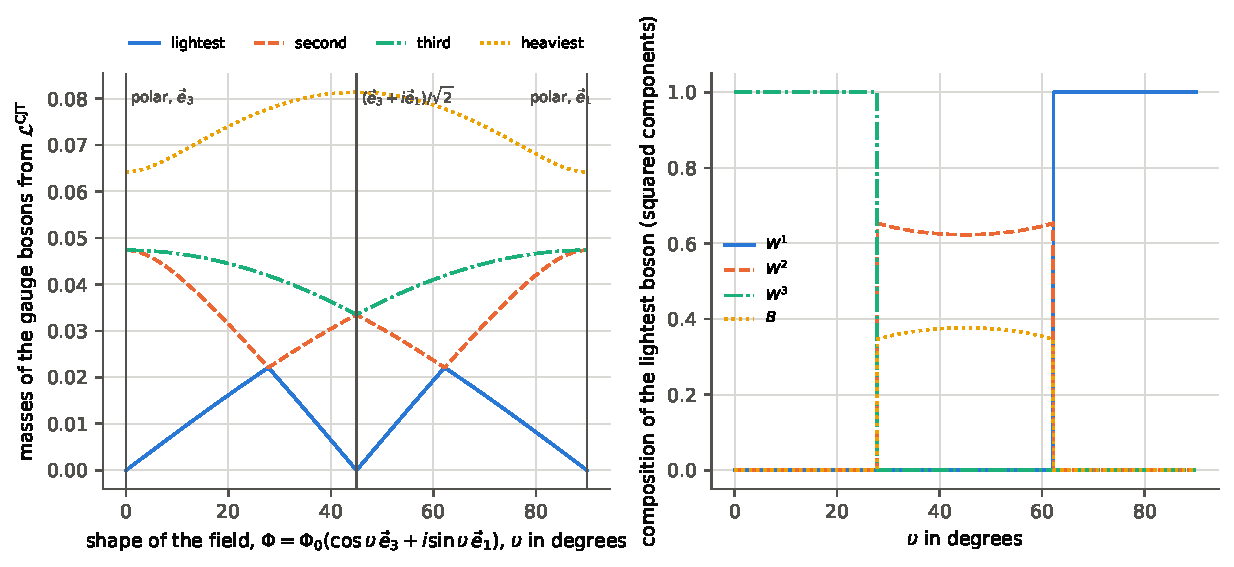
\includegraphics[width=0.85\textwidth]{figures/fig_part4_r1_massmatrix.pdf}
\caption{\label{fig:mixing}The mass matrix (\ref{eq:massmatrix}) of the effective Lagrangian of CJT along the fields
$\Phi_0(\cos\upsilon\,\vec e_3+i\sin\upsilon\,\vec e_1)$. Left: the four masses. Right: the squared components of the lightest boson. A
massless boson exists only where the field has a continuous stabilizer ($\upsilon=0$, $45^\circ$, $90^\circ$); at $\upsilon=45^\circ$ it is
$\cos\theta'W^2-\sin\theta'B$.}
\end{figure}

\paragraph*{The microscopic check.}
The same masses follow from the microscopic theory without the effective Lagrangian: the response of the self-consistent
vacuum to constant time components of the gauge fields (equivalently, to chemical potentials of the four charges) gives the
matrix $g_ag_b\chi^{ab}_\SF$. For the vacuum $\Phi_0e^{i\pi/5}\vec e_1$ (chosen so that the identification of the photon is not
trivial) its smallest eigenvalue vanishes to rounding ($8\times10^{-14}$ of the largest) with the eigenvector $W^1$, and the matrix agrees with
(\ref{eq:massmatrix}) to $3\times10^{-12}$ of $(M^X_{Z,\SF})^2$ in the five methods.

\paragraph*{The surviving group.}
The stabilizer of the vacuum $\Phi_0\vec e_3$ in GEE is $SL(2,\mathbb C)\times O(2)$, with
$O(2)=\{e^{i\theta T^3_\LL}\}\rtimes\{\mathsf 1,\mathsf r\}$, where $\mathsf r$ is the rotation by $\pi$ about $\vec e_1$ combined with the phase
$e^{i\pi F_\LL/2}$. Its identity component is the group $U(1)^{\rm Q}_\LL$ of the electric charge $Q_\LL=T^3_\LL$ (charges $\pm\frac12$
of the spinor field and $\pm1$ of $W^\pm$); $e^{2\pi iQ_\LL}$ and $e^{i\pi F_\LL}$ act alike on every field. $\mathsf r$ reverses $Q_\LL$
and acts on the gauge fields as $A\to-A$, $W^\pm\to W^\mp$, $Z\to Z$: a charge conjugation of the photon, without a gauge boson.
$SL(2,\mathbb C)$ is unbroken because the condensate is a Lorentz scalar.

\paragraph*{The count of the degrees of freedom and the Higgs mechanism in time.}
Before the breaking: four massless vector fields (8 polarizations) and six real components of $\vec\Phi$, together 14. After:
three massive vector fields (9), the photon (2), and three massive scalars ($h$ and the two non-unitary fields), together 14: the
three Goldstone fields have become the longitudinal polarizations of $W^\pm$ and $Z$. Keeping only the phase $\vartheta$ and $B$,
the Lagrangian $\frac12B_{01}^2+\frac12(f^{\rm F})^2[(\partial_0\vartheta+2g^{\rm F}_\LL B_0)^2-(\partial_1\vartheta-2g^{\rm F}_\LL B^1)^2]$ was integrated
in time in two gauges: in the temporal gauge with CVODE, and in the unitary gauge, where Gauss's law is an algebraic equation of
a differential-algebraic system of index one, with IDA~\cite{SUNDIALS2005,SUNDIALS2022}. A wave packet of the Goldstone field
that moves at the speed 1 without the gauge field becomes, with it, the longitudinal $Z$: its energy moves at the group velocity
$k/(k^2+M_Z^2)^{1/2}$ of the dispersion $\omega^2=k^2+M_Z^2$, and the two integrators agree on the gauge-invariant fields.

%=====================================================================================================================
\section{Finite temperature}
\label{sec:thermal}

\subsection{Thermal states and the free energy}

At the temperature $T$ the state is the thermal state $f(\mathsf H_\SF)$ of (\ref{eq:BdG}), $f(\varepsilon)=1/(e^{\varepsilon/T}+1)$, and its
free energy per volume is $\mathcal E^X_\SF-T\mathcal S_\SF$, with the energy of method $X$ (unchanged) and the entropy of the
quasi-free state,
\begin{equation}
\mathcal S_\SF=-\frac12\int\frac{d^3q}{(2\pi)^3}\sum_{k=1}^{16}\big[f_k\ln f_k+(1-f_k)\ln(1-f_k)\big],
\label{eq:entropy}
\end{equation}
where $f_k$ are the occupations of the 16 eigenvalues of $\mathsf H_\SF(\vec q)$; every mode appears twice (at $\pm\varepsilon$, with the
occupations $f$ and $1-f$), hence the factor $\frac12$. For HS this is the saddle point at finite $T$, for CJT the truncated effective
action at finite $T$~\cite{AmelinoCamelia1993}, and for KS Mermin's functional~\cite{Mermin1965} with the exchange-correlation
energy of $T=0$. The self-energies are the derivatives of the energy as at $T=0$, and the stationarity in the occupations gives
the Fermi function. The free energy of the field, $\mathcal F^X_\SF(\vec\Phi;T)$, is computed with an applied pair field as the
effective potential, and measured from the normal state at the same $T$.

\subsection{The critical temperature}

The normal state at $T$ has a normal self-energy that is a Dirac mass $M^{X,{\rm n}}_\SF(T)$ (the thermal particles and
antiparticles change the scalar density, which shifts the mass where $g^{X,{\rm S}}_\SF\ne0$). Its static pair response in the
channel $\mathsf K^3_\LL$ has the eigenvalue
\begin{equation}
\lambda^{\rm P}_\SF(T)=\frac{g^{X,{\rm P}}_\SF\,I_1\big(M^{X,{\rm n}}_\SF(T),T\big)}{\pi^2},\qquad I_1(M,T)=\int_0^{\Lambda_\LL}\frac{q^2\tanh(E/2T)}{E}dq,
\label{eq:lambdaT}
\end{equation}
($\tanh(E/2T)=1-2f(E)$ is the thermal factor of a pair of quasi-particles), and the critical temperature solves
$\lambda^{\rm P}_\SF(T^{X,{\rm c}}_\SF)=1$. In every method $\lambda^{\rm P}_\SF(T)$ does not increase with $T$ (checked on 60 temperatures from $0.01$
to $0.6$ in Rust and in the notebook and on 600 temperatures in Python), so $T^{X,{\rm c}}_\SF$ is unique; below it a polar start
ends in a superfluid, above it in the normal state. Table~\ref{tab:T0} gives $T^{X,{\rm c}}_\SF$.

\subsection{The gap equation, and the Dirac mass of the superfluid}

The polar superfluid at $T$ with the Dirac mass $M^{X,{\rm D}}_\SF$ and the order parameter $\Phi_0(T)$ has the pair self-consistency
(the gap equation)
\begin{equation}
1=\frac{g^{X,{\rm P}}_\SF}{\pi^2}\,I_1\big(E^{\rm gap}(T),T\big),\qquad E^{\rm gap}(T)=\big((M^{X,{\rm D}}_\SF)^2+\Phi_0(T)^2\big)^{1/2}.
\label{eq:gap}
\end{equation}
Its scalar density,
$n^{\rm S}=-\frac2{\pi^2}[M^{X,{\rm D}}_\SF I_1(E^{\rm gap},T)-m_\LL I_1(m_\LL,0)]$, contains the same integral, which (\ref{eq:gap}) fixes to
$\pi^2/g^{X,{\rm P}}_\SF$: $n^{\rm S}=-2M^{X,{\rm D}}_\SF/g^{X,{\rm P}}_\SF+2m_\LL I_1(m_\LL,0)/\pi^2$. The scalar self-consistency
$M^{X,{\rm D}}_\SF-m_\LL=g^{X,{\rm S}}_\SF n^{\rm S}$ therefore contains no temperature: \emph{the Dirac mass of the superfluid does not
depend on the temperature}, and $\Phi_0(T)$ follows from (\ref{eq:gap}) alone. Near $T^{X,{\rm c}}_\SF$ it vanishes like
$(1-T/T^{X,{\rm c}}_\SF)^{1/2}$. The ratio $E^{X,{\rm gap}}_\SF(0)/T^{X,{\rm c}}_\SF=1.65\mbox{--}1.74$ is of the size of the ratio 1.764 of the
theory of Bardeen, Cooper and Schrieffer~\cite{BCS1957}.

\subsection{The radius of convergence, and Landau's theory}

The free energy is an integral over the momenta of $-T\ln(2\cosh(E/2T))$ (one term per pair of eigenvalues $\pm E$) and of
densities with the factor $\tanh(E/2T)/E$. With the Matsubara frequencies $\omega_m=(2m+1)\pi T$,
\begin{equation}
\ln\big(2\cosh(E/2T)\big)=\ln2+\sum_{m=0}^\infty\ln\Big(1+\frac{E^2}{\omega_m^2}\Big),\qquad\frac{\tanh(E/2T)}{E}=4T\sum_{m=0}^\infty\frac1{\omega_m^2+E^2},
\label{eq:matsubara}
\end{equation}
functions of $\omega_m^2+q^2+M^2+\Phi_{\rm a}^2$. Integrated over the momenta, each is singular where $\omega_m^2+M^2+\Phi_{\rm a}^2=0$; the
nearest such point to the origin is $\Phi_{\rm a}^2=-(M^{X,{\rm n}}_\SF(T)^2+\pi^2T^2)$. The series of the free energy in $|\vec\Phi|^2$ about the
normal state therefore converges within a radius of the order of $r(T)=(M^{X,{\rm n}}_\SF(T)^2+\pi^2T^2)^{1/2}$, which grows with $T$.
Near $T^{X,{\rm c}}_\SF$ the order parameter lies well inside it, the residual of the Landau form falls to 0.00078\mbox{--}0.0017\% of the depth
at $0.98\,T^{X,{\rm c}}_\SF$, and the order parameter of Landau's theory, $(-a/2b)^{1/2}$ with the Taylor coefficients $a$, $b$ of
the free energy at the origin, has an error of relative order $1-T/T^{X,{\rm c}}_\SF$. These are statements about the mean-field free
energy; Sec.~\ref{sec:gi} shows that these temperatures lie inside the critical region.

\begin{table}[h]
\caption{\label{tab:T0}The five methods with $V^{(2)}_\SF$: effective couplings, the eigenvalue $\lambda^{\rm P}_\SF(0)$, the ground state at
$T=0$ (order parameter, Dirac mass, gap, depth of the effective potential), the critical temperature and the ratio of the gap
to it, in units of $\Lambda_\LL$. KS and CJT coincide on the polar states.}
\begin{ruledtabular}
\begin{tabular}{lrrrrrrrrr}
method & $g^{X,{\rm S}}_\SF$ & $g^{X,{\rm P}}_\SF$ & $\lambda^{\rm P}_\SF(0)$ & $\Phi^X_{0,\SF}$ & $M^{X,{\rm D}}_\SF$ & $E^{X,{\rm gap}}_\SF$ & $10^4|\mathcal V^X_\SF(\Phi_0)|$ & $T^{X,{\rm c}}_\SF$ & $E^{\rm gap}/T^{X,{\rm c}}_\SF$ \\
\hline
HS (1,1) & 2.80 & 25.2 & 1.1838 & 0.40306 & 0.20669 & 0.45297 & 5.186 & 0.26047 & 1.739 \\
HS (0,1) & 0 & 24.5 & 1.1510 & 0.36201 & 0.20000 & 0.41358 & 3.608 & 0.24047 & 1.720 \\
HS (0,0) & 0 & 23.7 & 1.1134 & 0.30699 & 0.20000 & 0.36639 & 2.062 & 0.21380 & 1.714 \\
KS & -7.40 & 23.7 & 1.1134 & 0.32849 & 0.16229 & 0.36639 & 2.422 & 0.22212 & 1.650 \\
CJT & -7.40 & 23.7 & 1.1134 & 0.32849 & 0.16229 & 0.36639 & 2.422 & 0.22212 & 1.650 \\
\end{tabular}
\end{ruledtabular}
\end{table}

%=====================================================================================================================
\section{The gradient coefficient at the critical temperature}
\label{sec:gradient}

\subsection{The functional of Ginzburg and Landau}

Near $T^{X,{\rm c}}_\SF$ the field is small. For a static field that varies slowly in space the free energy of method $X$, to second
order in the field and its derivatives and to fourth order in the field, is
\begin{equation}
\mathcal F^{X,{\rm GL}}_\SF=\int d^3x\Big[\mathsf c^X_\SF\sum_{j=1}^3(\partial_j\vec\Phi)^\dagger\cdot\partial_j\vec\Phi+\alpha^{X,{\rm GL}}_\SF t\,|\vec\Phi|^2+b^X_\SF|\vec\Phi|^4\Big],
\label{eq:GL}
\end{equation}
with the Taylor coefficient $a(0;T)\approx\alpha^{X,{\rm GL}}_\SF t$ of $|\vec\Phi|^2$ (so $\alpha^{X,{\rm GL}}_\SF=T^{X,{\rm c}}_\SF\partial_Ta$ at
$T^{X,{\rm c}}_\SF$) and the Taylor coefficient $b^X_\SF$ of $|\vec\Phi|^4$ at $T^{X,{\rm c}}_\SF$. Static fluctuations dominate near a continuous
transition: a fluctuation with the Matsubara frequency $2\pi mT$, $m\ne0$, costs of the order of $(2\pi T)^2$ times the coefficient of
the time derivatives, and $2\pi T^{X,{\rm c}}_\SF$ is 1.34\mbox{--}1.64, of the order of the cutoff. Rotations and isospin rotations allow no
other term of second order (the indices can only be contracted with $\delta_{jj'}$ and $\delta_{\iota\iota'}$), and a term with
$\vec\Phi\cdot\vec\Phi$ has the fermion number 4. At fourth order the two invariants $|\vec\Phi|^4$ and $|\vec\Phi\cdot\vec\Phi|^2$ are equal on
the polar fields (the minimum); (\ref{eq:GL}) keeps the coefficient along these fields.

\subsection{A moving pair: the twist}

A pair field with the momentum $q$ along $\vec e_3$, $\vec\Phi(\vec x)=\vec\Phi\,e^{iqx^3}$, has in (\ref{eq:GL}) the gradient term
$\mathsf c^X_\SF q^2|\vec\Phi|^2$, so its coefficient of $|\vec\Phi|^2$ is
\begin{equation}
a(q;T)=a(0;T)+\mathsf c^X_\SF q^2+O(q^4).
\label{eq:aq}
\end{equation}
Its state pairs the momenta $\vec q_\LL+\frac12q\vec e_3$ and $-\vec q_\LL+\frac12q\vec e_3$, with the relative momentum $\vec q_\LL$. The
gauge transformation $\Psi\to e^{iqx^3/2}\Psi$ makes the pair field uniform; since $\mathsf h_\LL(\vec q)$ is linear in $\vec q$, it replaces
$\mathsf h_\LL(\pm\vec q_\LL)$ in (\ref{eq:BdG}) by $\mathsf h_\LL(\pm\vec q_\LL)+\mathsf T^{\rm tw}$ with the \textbf{twist}
$\mathsf T^{\rm tw}=\frac12q\,\alpha^3_\LL\otimes\mathsf 1_2$. More generally, $Q\,\alpha^3_\LL\otimes\mathsf t$ with an isospin matrix $\mathsf t$ shifts
the momenta of the charges of $\mathsf t$: $\mathsf t=\mathsf 1_2$ moves the pair (fermion number 2) with $q=2Q$; $\mathsf t=\frac12\tau_1$ turns the
isospin direction of the field along $x^3$, moving its components of charge $\pm1$ of $T^1_\LL$ with the momenta $\pm Q$ (isospin
invariance requires the same coefficient); $\mathsf t=\frac12\tau_3$ twists the unbroken $T^3_\LL$, which does not change the field
$\Phi\vec e_3$ (its charge is 0) and should cost nothing (Sec.~\ref{sec:reg}). At second order in the field the normal self-energy
may be taken from the normal state at $T$: the free energy is stationary in it, so its change affects the free energy only at
fourth order.

\subsection{The static pair response}

Let $\mathsf H_0={\rm diag}(\mathsf A,\mathsf D)$ be the BdG matrix of the normal state with the twist, with the particle block
$\mathsf A=\mathsf h_\LL(\vec q_\LL)+\mathsf N^{\rm n}+\mathsf T$ (eigenvalues $\varepsilon^{\rm A}_a$, orthonormal eigenvectors $\mathsf u_a$) and the hole
block $\mathsf D=-(\mathsf h_\LL(-\vec q_\LL)+\mathsf N^{\rm n}+\mathsf T)^T$ (eigenvalues $\varepsilon^{\rm D}_b$, eigenvectors $\mathsf w_b$), and add a small
off-diagonal block, $\mathsf H=\mathsf H_0+\mathsf V$ with $\mathsf V=\begin{pmatrix}0&\mathsf P^{\rm a}\\(\mathsf P^{\rm a})^\dagger&0\end{pmatrix}$. The first-order
change of a function of a Hermitian matrix is (the formula of Daleckii and Krein): in the eigenbasis of $\mathsf H_0$ with the
eigenvalues $e_k$,
\begin{equation}
\big[\delta f(\mathsf H)\big]_{kl}=\frac{f(e_k)-f(e_l)}{e_k-e_l}\,\mathsf V_{kl},
\label{eq:dk}
\end{equation}
with $f'(e_k)$ where $e_k=e_l$. [It follows from the resolvent: $f(\mathsf H)=\oint\frac{dz}{2\pi i}f(z)(z-\mathsf H)^{-1}$ and
$\delta(z-\mathsf H)^{-1}=(z-\mathsf H_0)^{-1}\mathsf V(z-\mathsf H_0)^{-1}$, whose matrix element $\mathsf V_{kl}/((z-e_k)(z-e_l))$ integrates to the
divided difference.] The upper-right block of $f(\mathsf H)$ is $-\mathsf C^{\rm p}_\LL(\vec q_\LL)$, so the pair matrix summed over the momenta
is, to first order,
\begin{equation}
\mathsf C^{\rm p,tot}_\SF=\mathcal X^{\rm P}_\SF[\mathsf P^{\rm a}]=-\int\frac{d^3q_\LL}{(2\pi)^3}\sum_{a,b=1}^8\frac{f(\varepsilon^{\rm A}_a)-f(\varepsilon^{\rm D}_b)}{\varepsilon^{\rm A}_a-\varepsilon^{\rm D}_b}\,\mathsf u_a\mathsf u_a^\dagger\,\mathsf P^{\rm a}\,\mathsf w_b\mathsf w_b^\dagger .
\label{eq:chi}
\end{equation}
In the programs this is evaluated, at every node, for the 28 basis matrices $\mathsf E_{ab}-\mathsf E_{ba}$ ($a<b$) of the antisymmetric
$8\times8$ matrices: with $\mathsf U_{\rm A}=(\mathsf u_1,\dots,\mathsf u_8)$, $\mathsf U_{\rm D}=(\mathsf w_1,\dots,\mathsf w_8)$ and
$\mathsf F_{ab}=(f(\varepsilon^{\rm A}_a)-f(\varepsilon^{\rm D}_b))/(\varepsilon^{\rm A}_a-\varepsilon^{\rm D}_b)$, $\mathcal X^{\rm P}[\mathsf B]=-\sum_qw_q\mathsf U_{\rm A}
[(\mathsf U_{\rm A}^\dagger\mathsf B\mathsf U_{\rm D})\circ\mathsf F]\mathsf U_{\rm D}^\dagger$ (the circle is the entrywise product).

\subsection{The free energy at second order}

\emph{Claim:} the free energy of the state, measured from the normal state at $T$, is to second order in the pair field
\begin{equation}
\mathcal F^X_2=\tfrac12\,{\rm Re}\,\tr\Big[\big(\mathsf P^{\rm a}-\mathsf P_\SF[\mathsf C^{\rm p,tot}_\SF]\big)\big(\mathsf C^{\rm p,tot}_\SF\big)^\dagger\Big],
\label{eq:F2}
\end{equation}
where $\mathsf P_\SF[\cdot]$ is the pair self-energy (\ref{eq:Nbil}), (\ref{eq:Ppair}) of method $X$ for a given pair matrix (linear in it; it
contains every pair channel of the method's functional). \emph{Derivation.} (i) Consider the quadratic Hamiltonian $H_0+\epsilon V$
of the normal state plus a pair term $V$ whose BdG block is $\mathsf P^{\rm a}$. In the thermal state of $H_0+V$ the expectation value of
the pair term is $\langle V\rangle=-{\rm Re}\,\tr(\mathsf P^{\rm a}(\mathsf C^{\rm p,tot})^\dagger)$ (the pair block of the energy of a quasi-free
state). (ii) The thermodynamic potential $\Omega(\epsilon)=-T\ln{\rm Tr}\,e^{-(H_0+\epsilon V)/T}$ obeys $d\Omega/d\epsilon=\langle V\rangle_\epsilon$, and
$\langle V\rangle_\epsilon$ vanishes in the normal state and is linear in $\epsilon$ at this order, $\langle V\rangle_\epsilon=\epsilon\langle V\rangle$; hence
$\Omega(1)-\Omega(0)=\int_0^1\epsilon\,d\epsilon\,\langle V\rangle=\frac12\langle V\rangle$. (iii) The free energy of the method is this thermodynamic
potential minus $\langle V\rangle$ (the pair term is not part of the Hamiltonian of the model) plus the pair part $E_{\rm pair}$ of the
interaction energy of the method. $E_{\rm pair}$ is a quadratic form of the pair matrix whose derivative is the pair self-energy; for the
pairing term, for example, $E_{\rm pair}=-\frac14G_\LL w^{\rm P}|\tr(\mathsf K\mathsf C^T)|^2$ and, by (\ref{eq:Ppair}) and the antisymmetry of
$\mathsf K$, ${\rm Re}\,\tr(\mathsf P_\SF[\mathsf C]\mathsf C^\dagger)=\frac12G_\LL w^{\rm P}|\tr(\mathsf K\mathsf C^T)|^2$, so that
$E_{\rm pair}=-\frac12{\rm Re}\,\tr(\mathsf P_\SF[\mathsf C]\mathsf C^\dagger)$, and the same holds for the pair contractions of the bilinear terms. The
sum is $\frac12\langle V\rangle-\langle V\rangle+E_{\rm pair}=\frac12{\rm Re}\,\tr(\mathsf P^{\rm a}\mathsf C^\dagger)-\frac12{\rm Re}\,\tr(\mathsf P_\SF[\mathsf C]\mathsf C^\dagger)$,
which is (\ref{eq:F2}). The normal part of the energy does not change at second order, because the free energy is stationary in
the normal self-energy. $\square$ For a self-consistent pair field, $\mathsf P^{\rm a}=\mathsf P_\SF[\mathsf C^{\rm p,tot}]$, (\ref{eq:F2})
vanishes: a self-consistent pair field of infinitesimal amplitude exists exactly where the coefficient below changes sign.

\subsection{The free energy of the field}

The field of the state is the component of its own pair self-energy along $(\mathsf K^3_\LL)^\dagger$,
$\Phi^3=\tr(\mathsf K^3_\LL\mathsf P_\SF[\mathsf C^{\rm p,tot}])/8$. The free energy of the field is the smallest $\mathcal F^X_2$ among the states with
this field. The minimization at fixed field is done with a Lagrange multiplier: the components of $\mathsf P^{\rm a}$ along the three
$(\mathsf K^\iota_\LL)^\dagger$ (the three components of the field) are held at $(0,0,1)$, and its components along the other 25 basis
directions are made self-consistent, $\Pi_\perp\mathsf P^{\rm a}=\Pi_\perp\mathsf P_\SF[\mathcal X^{\rm P}[\mathsf P^{\rm a}]]$, where $\Pi_\perp$ removes the components
along the $(\mathsf K^\iota_\LL)^\dagger$. With the linear map $\mathsf M:\mathsf P^{\rm a}\mapsto\mathsf P_\SF[\mathcal X^{\rm P}[\mathsf P^{\rm a}]]$ on the 28 coefficients and
$\mathsf e_3$ the coefficients of $(\mathsf K^3_\LL)^\dagger$, this is the linear system
\begin{equation}
(\mathsf 1-\Pi_\perp\mathsf M)\,\mathsf p_\perp=\Pi_\perp\mathsf M\,\mathsf e_3,\qquad\mathsf P^{\rm a}=\mathsf e_3+\mathsf p_\perp ,
\label{eq:linsys}
\end{equation}
and then $a(q;T)=\mathcal F^X_2/|\Phi^3|^2$. At $q=0$ no other channel is induced ($|\mathsf p_\perp|\le${} $5\times10^{-16}$, checks P3-G4, YP3-G4, WP3-G4), and in the
channel $\mathsf K^3_\LL$ alone, where $\mathsf P_\SF[\mathsf C]=-\frac12g^{X,{\rm P}}_\SF\tr(\mathsf K^3_\LL\mathsf C^T)(\mathsf K^3_\LL)^\dagger$ (the definition of the effective
pair coupling) and the applied block $(\mathsf K^3_\LL)^\dagger$ produces the field $\lambda^{\rm P}_\SF(T)$ (the definition of the eigenvalue),
(\ref{eq:F2}) gives $\frac12(1-\lambda^{\rm P}_\SF)\cdot2\lambda^{\rm P}_\SF/g^{X,{\rm P}}_\SF$ for $|\Phi^3|^2=(\lambda^{\rm P}_\SF)^2$:
\begin{equation}
a(0;T)=\frac{1-\lambda^{\rm P}_\SF(T)}{\lambda^{\rm P}_\SF(T)\,g^{X,{\rm P}}_\SF},\qquad\alpha^{X,{\rm GL}}_\SF=-\frac{T^{X,{\rm c}}_\SF}{g^{X,{\rm P}}_\SF}\frac{d\lambda^{\rm P}_\SF}{dT}\Big|_{T^{X,{\rm c}}_\SF}.
\label{eq:a0}
\end{equation}
The derivative is evaluated in closed form, $d\lambda^{\rm P}/dT=(g^{X,{\rm P}}_\SF/\pi^2)(\partial_TI_1+\partial_MI_1\,dM^{X,{\rm n}}_\SF/dT)$ with
\begin{equation}
\partial_TI_1=-\frac1{2T^2}\int_0^{\Lambda_\LL}\frac{q^2\,dq}{\cosh^2(E/2T)},\qquad\partial_MI_1=\int_0^{\Lambda_\LL}q^2\frac{M}{E}\Big[\frac1{2TE\cosh^2(E/2T)}-\frac{\tanh(E/2T)}{E^2}\Big]dq,
\label{eq:dI}
\end{equation}
and $dM^{X,{\rm n}}_\SF/dT=g^{X,{\rm S}}_\SF\partial_Tn^{\rm S}/(1-g^{X,{\rm S}}_\SF\partial_Mn^{\rm S})$ from the scalar self-consistency
$M-m_\LL=g^{X,{\rm S}}_\SF n^{\rm S}(M,T)$, $n^{\rm S}=-\frac2{\pi^2}[MI_1(M,T)-m_\LL I_1(m_\LL,0)]$ (the implicit function theorem). The Rust program
and the notebook compare this closed form with the central differences of $a(0;T)$ at $T^{X,{\rm c}}_\SF(1\pm0.002)$ and $(1\pm0.004)$
(Richardson extrapolation), and the Python program compares its closed form with the value of the Rust program: they agree to
$7\times10^{-12}$ (checks P3-G10, WP3-G10, YP3-G10).

\subsection{The regularization of a moving pair}
\label{sec:reg}

The model restricts the momenta of the uniform states to $|\vec q_\LL|<\Lambda_\LL$; for a moving pair the cutoff must be placed on one
of two momenta. \emph{The cutoff on the momenta of the two charges}, $|\vec q_\LL\pm\frac12q\vec e_3|<\Lambda_\LL$, restricts the relative
momenta to a lens, the intersection of two balls whose centres are $q$ apart. The lens lacks, compared with the ball
$|\vec q_\LL|<\Lambda_\LL$, a shell at the cutoff of the thickness $\frac12q|\cos\theta|$ in the direction $\theta$ (its radius is
$-\frac12q|n_3|+(\Lambda_\LL^2-\frac14q^2(1-n_3^2))^{1/2}$ in the direction $\vec n$), whose volume is of first order in $|q|$. The pairs in that shell
contribute to $a$ at first order, and
\begin{equation}
a_{\rm lens}(q;T)-a(0;T)\propto|q|,
\label{eq:lens}
\end{equation}
so that the expansion (\ref{eq:aq}) does not exist: doubling $q$ from 0.005 to 0.01 multiplies the change by 2.014\mbox{--}2.015 (a
linear function gives 2; Fig.~\ref{fig:gi}a). \emph{The cutoff on the relative momentum}, $|\vec q_\LL|<\Lambda_\LL$, keeps the ball, and
the change is quadratic (the factor is $4.0000$ to five digits). This is the routing of the momenta of the twisted states of
Sec.~\ref{sec:T0}, where a uniform twist shifts the momenta inside the fixed ball, and it is used here. Two quantities measure the
remaining error of the regularization:
\begin{enumerate}
\item the twist $Q\,\alpha^3_\LL\otimes\frac12\tau_3$ of the unbroken generator $T^3_\LL$ costs the spurious coefficient $\mathsf c^{X,{\rm T3}}_\SF$, which
is 18\mbox{--}21\% of $\mathsf c^X_\SF$ (Table~\ref{tab:gi}); the isospin twist gives the same coefficient as the phase twist to $3\times10^{-11}$ in the Rust program and the notebook and to
$4\times10^{-10}$ in the Python program (checks P3-G5, WP3-G5, YP3-G5);
\item the nonlinear thermal states of the engine with the constant twist and a self-consistent normal self-energy give a
coefficient $\mathsf c^{X,{\rm tw}}_\SF$ that agrees with the linear response with the pair self-energy along $(\mathsf K^3_\LL)^\dagger$ to
$2.4\times10^{-6}$ for HS $(0,0)$, which has no normal self-energy ($4\times10^{-7}$ in the Python program; checks P3-G7, YP3-G7), but differs by 10\mbox{--}11\% in HS $(1,1)$, HS $(0,1)$ and KS and by
$-$60\% in CJT: the twisted normal state carries a spurious current (the occupied ball is displaced), which through the vector
interaction changes the normal self-energy at first order in $q$. The linear response (\ref{eq:chi}) uses the normal self-energy of
the untwisted normal state and is free of this effect, because a moving pair field changes the normal self-energy only at second
order in the field.
\end{enumerate}

\subsection{The numerical method}

$\mathsf c^X_\SF$ is $[a(q;T^{X,{\rm c}}_\SF)-a(0;T^{X,{\rm c}}_\SF)]/q^2$ at $q=0.01$ and $0.02$ with the Richardson extrapolation (the two values
differ by at most $3\times10^{-5}$ of $\mathsf c$). The six directions are exact at second order in $q$ (the term of second order of the integrand
is a polynomial of degree two in the direction, which the six-direction rule integrates exactly); a product rule of 64 directions
and a grid of 40 radial nodes give $\mathsf c^{\rm CJT}_\SF$ to $2\times10^{-10}$ (check P3-G8), the Python program on 64 directions gives every
$\mathsf c^X_\SF$ to $3\times10^{-10}$ (YP3-G8), and the notebook gives every $\mathsf c^X_\SF$ on the grid of six directions to $6\times10^{-11}$ of the
value of the Rust program (WP3-G6) and $\mathsf c^{\rm CJT}_\SF$ on a product rule of 144 directions to $2\times10^{-10}$ (WP3-G8). $b^X_\SF$ comes from the nonlinear free
energy of four states with the applied fields $0.01$ to $0.04$ at $T^{X,{\rm c}}_\SF$ ($\mathcal F/\Phi^2$ interpolated by a cubic polynomial in
$\Phi^2$); the fields $0.015$ to $0.045$ give the same value to $10^{-7}$ (check P3-G12). Table~\ref{tab:gi} gives the results.

\begin{table}[h]
\caption{\label{tab:gi}The coefficients of (\ref{eq:GL}) at the critical temperature: the critical temperature, the Dirac mass of
the normal state, $\alpha$, $b$, the gradient coefficient from the phase twist (the result), from the isospin twist, without the
other pair channels, the spurious coefficient of the $T^3_\LL$ twist and the coefficient of the twisted nonlinear states; the
correlation length, the specific-heat jump per correlation volume, the Ginzburg number (\ref{eq:Gi}), the width of the critical
region in temperature, and the Ginzburg number with $\mathsf c$ changed by $\pm\mathsf c^{\rm T3}$.}
\begin{ruledtabular}
\begin{tabular}{lrrrrr}
quantity & HS (1,1) & HS (0,1) & HS (0,0) & KS & CJT \\
\hline
$T^{X,{\rm c}}_\SF$ & 0.260467 & 0.240465 & 0.213799 & 0.222119 & 0.222119 \\
$M^{X,{\rm n}}_\SF(T^{X,{\rm c}}_\SF)$ & 0.206685 & 0.200000 & 0.200000 & 0.162293 & 0.162293 \\
$10^2\alpha^{X,{\rm GL}}_\SF$ & 1.40379 & 1.26991 & 1.07434 & 1.11755 & 1.11755 \\
$10^2b^X_\SF$ & 1.23886 & 1.37640 & 1.59434 & 1.47237 & 1.47237 \\
$10^2\mathsf c^X_\SF$ (phase twist) & 1.54875 & 1.71376 & 1.95280 & 1.92718 & 1.92718 \\
$10^2\mathsf c$ (isospin twist) & 1.54875 & 1.71376 & 1.95280 & 1.92718 & 1.92718 \\
$10^2\mathsf c$ (other channels held at 0) & 1.54875 & 1.71380 & 1.95281 & 1.92718 & 1.92718 \\
$10^2\mathsf c^{X,{\rm T3}}_\SF$ (twist of $T^3_\LL$) & 0.3218 & 0.3395 & 0.3597 & 0.3597 & 0.3597 \\
$10^2\mathsf c^{X,{\rm tw}}_\SF$ (twisted states) & 1.723 & 1.905 & 1.953 & 2.121 & 0.7684 \\
$\xi=(\mathsf c/\alpha)^{1/2}$ & 1.050 & 1.162 & 1.348 & 1.313 & 1.313 \\
$\Delta C\,\xi^3$ & 0.0354 & 0.0382 & 0.0415 & 0.0432 & 0.0432 \\
${\rm Gi}^X_\SF$ & 11.38 & 9.768 & 8.277 & 7.621 & 7.621 \\
${\rm Gi}^X_\SF T^{X,{\rm c}}_\SF$ & 2.964 & 2.349 & 1.770 & 1.693 & 1.693 \\
Gi with $\mathsf c\mp\mathsf c^{\rm T3}$ & 6.46--22.9 & 5.68--18.9 & 4.98--15.2 & 4.56--14.2 & 4.56--14.2 \\
\end{tabular}
\end{ruledtabular}
\end{table}

\begin{figure}[h]
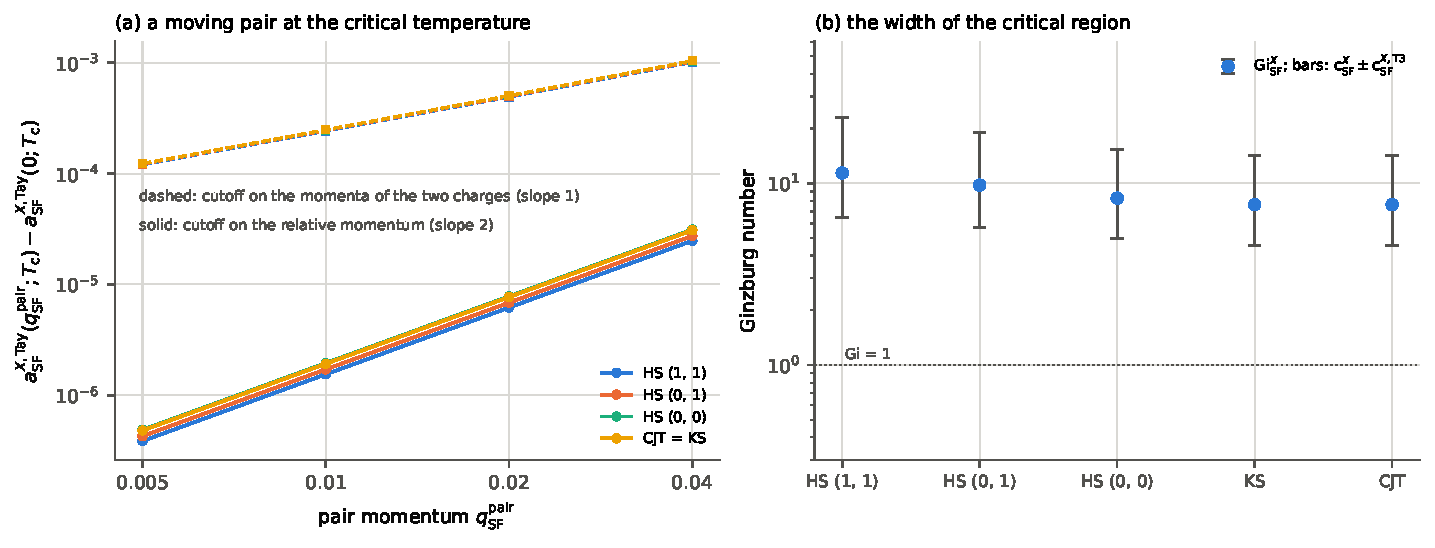
\includegraphics[width=0.85\textwidth]{figures/fig_prd_ginzburg.pdf}
\caption{\label{fig:gi}(a) $a(q;T^{X,{\rm c}}_\SF)-a(0;T^{X,{\rm c}}_\SF)$ against the momentum $q$ of the pair for the two regularizations:
quadratic for the cutoff on the relative momentum (solid), linear for the cutoff on the momenta of the two charges (dashed). (b) The
Ginzburg number (\ref{eq:Gi}) of the five methods, with the range for $\mathsf c^X_\SF$ changed by $\pm\mathsf c^{X,{\rm T3}}_\SF$, against
${\rm Gi}=1$.}
\end{figure}

%=====================================================================================================================
\section{The Ginzburg number}
\label{sec:gi}

Above $T^{X,{\rm c}}_\SF$ the field fluctuates about zero with the probability density proportional to $\exp(-\mathcal F^{X,{\rm GL}}_\SF/T)$. To
second order the weight is Gaussian; in a volume $V$ with periodic boundary conditions each of the $n=6$ real components and each
wave vector $\vec k$ contributes a factor $\int d\phi\,e^{-V(\mathsf ck^2+a)\phi^2/T}\propto(\mathsf ck^2+a)^{-1/2}$, so the free energy per volume
of the fluctuations is, up to terms analytic in $T$,
\begin{equation}
\mathcal F^{\rm fl}=\frac n2T\int\frac{d^3k}{(2\pi)^3}\ln\big(\mathsf ck^2+a\big),\qquad a=\alpha t,\ \ \partial_Ta=\frac{\alpha}{T^{X,{\rm c}}_\SF}.
\label{eq:Ffl}
\end{equation}
Its second derivative in $T$ near $T^{X,{\rm c}}_\SF$ is dominated by the term with the second derivative of the logarithm,
$-\frac n2T(\partial_Ta)^2\int\frac{d^3k}{(2\pi)^3}(\mathsf ck^2+a)^{-2}$, and with
\begin{equation}
\int\frac{d^3k}{(2\pi)^3}\frac1{(\mathsf ck^2+a)^2}=\frac1{2\pi^2}\int_0^\infty\frac{k^2dk}{(\mathsf ck^2+a)^2}=\frac{1}{8\pi\,\mathsf c^{3/2}a^{1/2}}
\label{eq:integral}
\end{equation}
(substitute $k=(a/\mathsf c)^{1/2}u$ and use $\int_0^\infty u^2(1+u^2)^{-2}du=\pi/4$), the specific heat per volume
$C=-T\partial_T^2\mathcal F$ of the fluctuations is
\begin{equation}
C^{\rm fl}=\frac{n\,\alpha^{3/2}}{16\pi\,\mathsf c^{3/2}\,t^{1/2}},
\label{eq:Cfl}
\end{equation}
divergent at $T^{X,{\rm c}}_\SF$. Below $T^{X,{\rm c}}_\SF$ the minimum of (\ref{eq:GL}) is $|\vec\Phi|^2=-a/(2b)$ with the free energy $-a^2/(4b)$ per
volume, so the specific heat of mean-field theory jumps at $T^{X,{\rm c}}_\SF$ by
\begin{equation}
\Delta C=T^{X,{\rm c}}_\SF\,\frac{(\partial_Ta)^2}{2b}=\frac{\alpha^2}{2b\,T^{X,{\rm c}}_\SF}.
\label{eq:DC}
\end{equation}
Mean-field theory holds where $C^{\rm fl}\ll\Delta C$. The two are equal at $t={\rm Gi}^X_\SF$,
\begin{equation}
{\rm Gi}^X_\SF=\frac{n^2b^2(T^{X,{\rm c}}_\SF)^2}{64\pi^2\,\alpha\,\mathsf c^3}=\frac{n^2}{256\pi^2\,(\Delta C\,\xi^3)^2},\qquad\xi=\Big(\frac{\mathsf c}{\alpha}\Big)^{1/2},
\label{eq:Gi}
\end{equation}
the Ginzburg number~\cite{Levanyuk1959,Ginzburg1960}; the second form follows from $\Delta C\xi^3=\alpha^{1/2}\mathsf c^{3/2}/(2bT^{X,{\rm c}}_\SF)$. The
correlation length of mean-field theory is $\xi|t|^{-1/2}$, and mean-field theory needs a large specific-heat jump per correlation
volume, $\Delta C\xi^3\gg1$: many degrees of freedom in a correlation volume. \emph{A remark on the factors.} Other forms of the
criterion (the mean square fluctuation of the field in a correlation volume against the square of its mean value, or the first
correction to $b$ against $b$) give the same combination of $\alpha$, $b$, $\mathsf c$ and $T_{\rm c}$ with other numerical factors of order
one. (\ref{eq:Gi}) is the definition used here; a factor of order one does not change the conclusion, because the numbers are far
above 1.

\paragraph*{The result.} ${\rm Gi}^X_\SF=7.6\mbox{--}11$ (Table~\ref{tab:gi}). Even at $|t|=1$ the Gaussian fluctuations alone give
$C^{\rm fl}/\Delta C=({\rm Gi}^X_\SF)^{1/2}=2.8\mbox{--}3.4$; the width ${\rm Gi}^X_\SF T^{X,{\rm c}}_\SF$ of the critical region exceeds
$T^{X,{\rm c}}_\SF$. The correlation length $\xi=1.05\mbox{--}1.35$ is about the shortest length $1/\Lambda_\LL$ of the model: the pairs are tightly
bound (there is no Fermi surface, the chemical potential is zero, and the coupling is above the critical one), and a correlation
volume holds $\Delta C\xi^3=0.035\mbox{--}0.043$ degrees of freedom. In a superconductor of Bardeen, Cooper and Schrieffer the correlation
length is large against the distance of the electrons and ${\rm Gi}\sim(T_{\rm c}/E_{\rm F})^4$ with the Fermi energy $E_{\rm F}$ is tiny; here
the opposite holds. With $\mathsf c$ changed by $\pm\mathsf c^{\rm T3}$, ${\rm Gi}^X_\SF$ lies between 4.6 and 23. The temperatures at
which the mean-field free energy behaves as Landau's theory (Sec.~\ref{sec:thermal}) lie inside the critical region, and the
mean-field statements near $T^{X,{\rm c}}_\SF$ (the critical temperature, the exponent $\frac12$, the continuity of the transition) are
not reliable.

%=====================================================================================================================
\section{The superfluid as a Higgs sector}
\label{sec:higgs}

\subsection{The Standard Model and the analogue of the vacuum value}

The Standard Model has $M_W=gv/2$, $M_Z=(g^2+g'^2)^{1/2}v/2$, $v=(\sqrt2G_F)^{-1/2}=246.22$~GeV, $m_H=125.20\pm0.11$~GeV,
$\Gamma_H=3.7^{+1.9}_{-1.4}$~MeV, $M_W=80.3692\pm0.0133$~GeV, $M_Z=91.1880\pm0.0020$~GeV~\cite{PDG2024}, and the quartic coupling
$\lambda_H=m_H^2/(2v^2)=0.1293$ (the convention $m_H^2=2\lambda_Hv^2$). By (\ref{eq:MWMZ}) the analogue of $v$ is
\begin{equation}
v^X_\SF=2f^{X,{\rm I}}_\SF,\qquad M^X_{W,\SF}=\tfrac12g^{\rm v}_\LL v^X_\SF,\qquad\lambda^{X,{\rm H}}_\SF=\frac{(M^{X,{\rm H}}_\SF)^2}{2(v^X_\SF)^2},
\label{eq:vSF}
\end{equation}
independent of the gauge coupling. The scale $\Lambda_\LL$ on which $v^X_\SF=246.22$~GeV is $246.22~{\rm GeV}/v^X_\SF$.

\subsection{The couplings of the amplitude field and the width}

On the field $\vec\Phi=(\Phi_0+h/N_h)e^{i\vartheta_0}\vec e_3$ with $N_h=(2(Z+Y))^{1/2}$ (so that $h$ is canonically normalized), both invariants
of (\ref{eq:Lkin}) equal $(\Phi_0+h/N_h)^2(\partial\vartheta_0)^2$, and the term linear in $h$ is $2(Z+Y)\Phi_0(\partial\vartheta_0)^2h/N_h=
f^{X,{\rm F}}_\SF h(\partial\vartheta_0)^2$. On the field rotated about $\vec e_1$ by $\vartheta_1$, $\vec\Phi^\dagger\cdot\partial\vec\Phi=0$ and only the first
invariant contributes: $2Z\Phi_0(\partial\vartheta_1)^2h/N_h=((f^{X,{\rm I}}_\SF)^2/f^{X,{\rm F}}_\SF)h(\partial\vartheta_1)^2$, and likewise for $\vartheta_2$.
(The notebook derives these two couplings by exact symbolic differentiation; the Python program by finite differences of the field.)
With the canonical Goldstone fields $\pi_0=f^{X,{\rm F}}_\SF\vartheta_0$ and $\pi_k=f^{X,{\rm I}}_\SF\vartheta_k$ all three couplings are
$h(\partial\pi)^2/f^{X,{\rm F}}_\SF$. For the decay of $h$ at rest (four-momentum $P$, $P^2=M_H^2$) into two massless quanta of one field
with the four-momenta $k_1,k_2$, the vertex $g\,h\,\partial_\mu\pi\partial^\mu\pi$ with $g=1/f^{X,{\rm F}}_\SF$ gives the amplitude
$\mathcal M=-2g\,k_1\cdot k_2=-g\,M_H^2$ (two contractions; $2k_1\cdot k_2=P^2$ for massless quanta), and with the two-body phase space
of two identical particles, $\Gamma=|\mathcal M|^2/(32\pi M_H)$:
\begin{equation}
\Gamma(h\to\pi\pi)=\frac{M_H^3}{32\pi(f^{X,{\rm F}}_\SF)^2},\qquad\Gamma^{X,{\rm H}}_\SF=\frac{3\,(M^{X,{\rm H}}_\SF)^3}{32\pi\,(f^{X,{\rm F}}_\SF)^2}
\label{eq:width}
\end{equation}
for the three channels. With the gauge fields the Goldstone fields are the longitudinal parts of $W^\pm$ and $Z$, and by the
equivalence theorem~\cite{CLT1974,ChanowitzGaillard1985} (\ref{eq:width}) is the width into $W^+W^-$ and $ZZ$ up to corrections of relative order
$x=M_V^2/M_H^2$, where $M_V$ is the mass of $W$ or $Z$: at tree level the width of a scalar with the couplings of (\ref{eq:Lkin})
into a pair of these bosons carries the factor $(1-4x)^{1/2}(1-4x+12x^2)$ (phase space and the sum over the polarizations), which
is above 0.93 here ($M_V\le0.11\,M_H$). For the Standard Model with
$f=v$, (\ref{eq:width}) is the known width $3m_H^3/(32\pi v^2)$ of a heavy Higgs boson~\cite{LQT1977}. \emph{A remark:} the effective
Lagrangian is used at the energy $M^{X,{\rm H}}_\SF$, where it is not accurate (its mass of the amplitude mode differs from the response
by 7.0\mbox{--}17\%); (\ref{eq:width}) gives the order of magnitude, which is all that the conclusion needs.

\begin{table}[h]
\caption{\label{tab:higgs}The superfluid as a Higgs sector (units of $\Lambda_\LL$; gauge boson masses at $g^{\rm v}_\LL=0.7$,
$g^{\rm F}_\LL=0.45$; the last rows set $v^X_\SF=246.22$~GeV), and the Standard Model~\cite{PDG2024}, whose thermal crossover is at
$159.5\pm1.5$~GeV~\cite{DOnofrio2016}.}
\begin{ruledtabular}
\begin{tabular}{lcccccc}
quantity & HS (1,1) & HS (0,1) & HS (0,0) & KS & CJT & Standard Model \\
\hline
$v^X_\SF=2f^{X,{\rm I}}_\SF$ & 0.1431 & 0.1354 & 0.1228 & 0.1314 & 0.1353 & 246.22 GeV \\
$f^{X,{\rm F}}_\SF$ & 0.07097 & 0.06723 & 0.06139 & 0.07135 & 0.07135 & -- \\
$M^{X,{\rm H}}_\SF$ (amplitude mode) & 0.8137 & 0.7251 & 0.6144 & 0.6035 & 0.6035 & 125.20 GeV \\
$M^{X,{\rm NU}}_\SF$ (charged scalars) & 0.8061 & 0.7251 & 0.6144 & 0.6573 & 0.6440 & -- \\
$M^X_{W,\SF}$ & 0.0501 & 0.0474 & 0.0430 & 0.0460 & 0.0474 & 80.37 GeV \\
$M^X_{Z,\SF}$ & 0.0639 & 0.0605 & 0.0553 & 0.0642 & 0.0642 & 91.19 GeV \\
$M^{X,{\rm H}}_\SF/v^X_\SF$ & 5.69 & 5.35 & 5.00 & 4.59 & 4.46 & 0.5085 \\
$\lambda^{X,{\rm H}}_\SF$ & 16.2 & 14.3 & 12.5 & 10.5 & 9.94 & 0.1293 \\
$M^{X,{\rm H}}_\SF/M^X_{W,\SF}$ & 16.2 & 15.3 & 14.3 & 13.1 & 12.7 & 1.558 \\
$M^X_{W,\SF}/M^X_{Z,\SF}$ & 0.784 & 0.783 & 0.778 & 0.716 & 0.738 & 0.8814 \\
$M^{X,{\rm H}}_\SF/2E^{X,{\rm gap}}_\SF$ & 0.898 & 0.877 & 0.838 & 0.824 & 0.824 & -- \\
$M^{X,{\rm NU}}_\SF/M^{X,{\rm H}}_\SF$ & 0.991 & 1.00 & 1.00 & 1.09 & 1.07 & none \\
$f^{X,{\rm F}}_\SF/f^{X,{\rm I}}_\SF$ & 0.992 & 0.993 & 1.00 & 1.09 & 1.05 & -- \\
$\Gamma^{X,{\rm H}}_\SF/M^{X,{\rm H}}_\SF$, Eq.~(\ref{eq:width}) & 3.9 & 3.5 & 3.0 & 2.1 & 2.1 & $3\times10^{-5}$ \\
$T^{X,{\rm c}}_\SF/v^X_\SF$ & 1.82 & 1.78 & 1.74 & 1.69 & 1.64 & 0.648 \\
$\Lambda_\LL$ [GeV] & 1721 & 1818 & 2005 & 1874 & 1820 & -- \\
$M^{X,{\rm H}}_\SF$ [GeV] & 1400 & 1318 & 1232 & 1131 & 1098 & 125.20 \\
$T^{X,{\rm c}}_\SF$ [GeV] & 448 & 437 & 429 & 416 & 404 & 159.5 \\
${\rm Gi}^X_\SF$, Eq.~(\ref{eq:Gi}) & 11.4 & 9.77 & 8.28 & 7.62 & 7.62 & -- \\
\end{tabular}
\end{ruledtabular}
\end{table}

\begin{figure}[h]
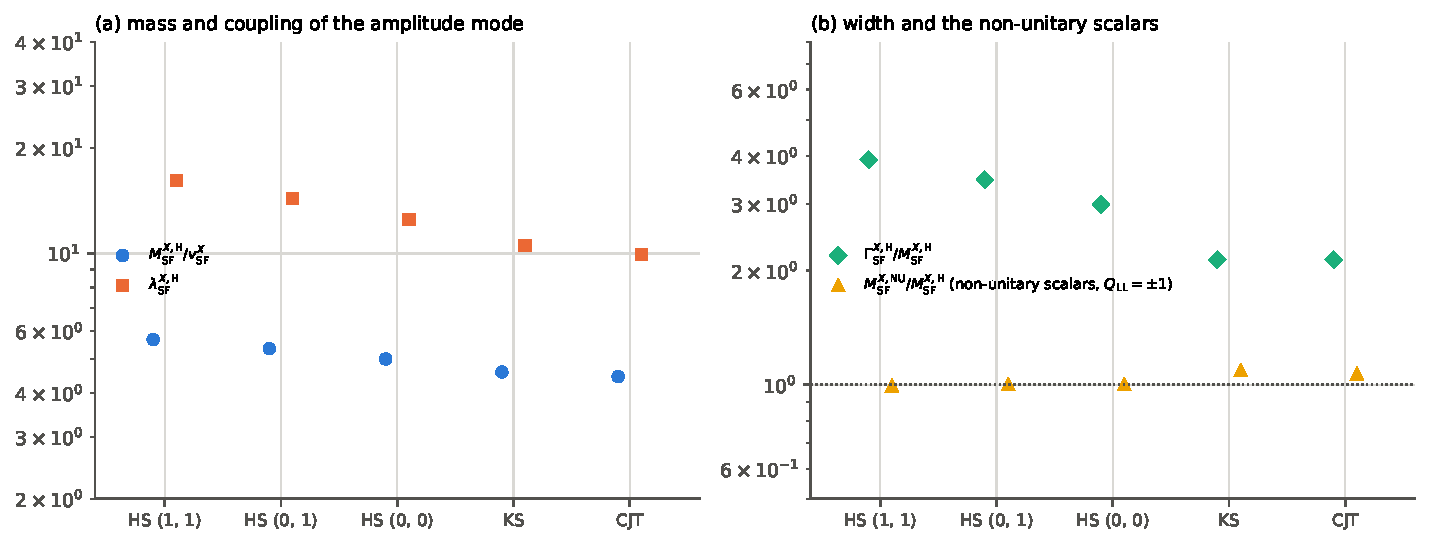
\includegraphics[width=0.85\textwidth]{figures/fig_prd_higgs.pdf}
\caption{\label{fig:higgs}(a) $M^{X,{\rm H}}_\SF/v^X_\SF$ and $\lambda^{X,{\rm H}}_\SF$ of the five methods against the Standard Model (dashed) and
the tree-level bound $8\pi/3$ of perturbative unitarity (dotted). (b) The width (\ref{eq:width}) relative to the mass, against
$\Gamma_H/m_H$ of the Standard Model, and the mass ratio $M^{X,{\rm NU}}_\SF/M^{X,{\rm H}}_\SF$ of the charged scalars.}
\end{figure}

\subsection{The verdict}

Seven properties of the Higgs sector of the Standard Model decide (Table~\ref{tab:higgs}):
(1) the Higgs mechanism, with a massless photon: realized in every method (Sec.~\ref{sec:mass});
(2) a neutral scalar below threshold: in every method, at 0.82\mbox{--}0.90 of $2E^{X,{\rm gap}}_\SF$;
(3) its mass against the scale of the breaking: $M^{X,{\rm H}}_\SF/v^X_\SF=4.46\mbox{--}5.69$, 8.8\mbox{--}11 times the value of the Standard Model, and
$\lambda^{X,{\rm H}}_\SF=9.94\mbox{--}16.2$, above the tree-level bound $8\pi/3=8.38$ of perturbative unitarity of the scattering of
longitudinal gauge bosons~\cite{LQT1977};
(4) its width: $\Gamma^{X,{\rm H}}_\SF/M^{X,{\rm H}}_\SF=2.1\mbox{--}3.9$, a broad resonance, against $\Gamma_H/m_H\approx3\times10^{-5}$;
(5) no further scalars: every method has the charged non-unitary doublet at 0.991\mbox{--}1.09 of $M^{X,{\rm H}}_\SF$;
(6) the quantum numbers: an isospin vector of fermion number 2 of a vector-like isospin instead of a hypercharge doublet of the chiral
$SU(2)_L$; the photon is $W^3$, the $Z$ is the boson of the fermion number, $M_W/M_Z$ depends on two independent couplings without a
custodial relation, and the condensate adds a pairing gap to the Dirac mass rather than generating Yukawa masses;
(7) the thermal history: the transition lies deep in its critical region (Sec.~\ref{sec:gi}), while the Standard Model has a smooth
crossover. In no method can the amplitude mode be the observed Higgs boson; CJT and KS come closest, HS $(1,1)$ is farthest.

%=====================================================================================================================
\section{Compositeness}
\label{sec:composite}

The field $\vec\Phi^X_\SF$ is not a field of the Lagrangian (\ref{eq:L}), whose only matter field is the spinor field: it is the amplitude
(\ref{eq:Phi}) of the pair self-energy, a composite of two spinor charges. Its kinetic part has no term of its own: $Z^X_\SF$ and $Y^X_\SF$
are susceptibilities of the spinor field, Eq.~(\ref{eq:ZY}). Its amplitude mode is a bound state of two quasi-particles below their
threshold. This is the compositeness condition of Bardeen, Hill and Lindner~\cite{BHL1990}: the normalization of the kinetic term of the
composite field vanishes at the cutoff, where only the spinor field exists. In the dynamics of Nambu and
Jona-Lasinio~\cite{NJL1961} the mass of the bound state is tied to the gap of its constituents (here $M^{X,{\rm H}}_\SF$ is 0.82\mbox{--}0.90
of $2E^{X,{\rm gap}}_\SF$), while the scale of the breaking comes from a loop of the constituents and is small against the gap
($f^{X,{\rm I}}_\SF/E^{X,{\rm gap}}_\SF=0.16\mbox{--}0.18$): the composite is heavy against $v$. A light composite Higgs needs a cutoff far above the
gap~\cite{BHL1990,HillSimmons2003} or a different mechanism, such as a pseudo-Goldstone Higgs~\cite{KaplanGeorgi1984,Agashe2005}.
Whether the Higgs boson of nature is composite is not decided here: its couplings agree with those of the Standard Model to several
per cent~\cite{ATLAS2022,CMS2022}, which constrains, but does not exclude, compositeness at a higher scale.

\paragraph*{The vacuum energy.} The condensate lowers the energy density of the vacuum by the depth of the effective potential,
$2.4\times10^{-4}\,\Lambda_\LL^4$ in CJT, about $(227~{\rm GeV})^4$ on the scale of Table~\ref{tab:higgs}, against the observed
dark-energy density of about $2.5\times10^{-47}~{\rm GeV}^4$: the cosmological-constant problem~\cite{Weinberg1989} in its usual form.

%=====================================================================================================================
\section{Toward the gravitational sector: Lord's construction}
\label{sec:gravity}

The article states a program, not a result; this section describes the construction on which it rests. Lord~\cite{Lord1971} considered
the two-component spinor algebra and the group of changes of its representation, under which the free field equations of particles of
any spin (written with two-component spinors) are invariant. Making this group local, in the manner of Yang and Mills, requires a gauge
field; gauge invariance together with Lorentz covariance then requires auxiliary fields. Lord interpreted the auxiliary fields as the
potentials of a spin-two field, which is therefore self-interacting, and showed that the Bargmann-Wigner equations of the linear spin-two
field, modified by this self-interaction, give a nonlinear theory identical with Einstein's general relativity. In addition the auxiliary
fields become the gauge field of the general coordinate transformations: the components of the affine connection. The construction is the
natural route for the present model because its spinor charges come with $SL(2,\mathbb C)$ from the super-loop~\cite{Nash2026}, and GEE
already contains $SL(2,\mathbb C)$ as a gauge factor with the connection $\Gamma^\LL_p$ of (\ref{eq:cov}), which on the flat space-time of
the article is a pure gauge. The program is: (i) replace the pure-gauge $\Gamma^\LL_p$ by Lord's gauge field and its auxiliary fields;
(ii) couple the spinor field and its pairs to it; (iii) derive the gravitational field equations with the energy-momentum tensor of the
spinor field, including the condensate, as their source. Two consequences of the present results are already clear: the superfluid is a
Lorentz scalar and leaves $SL(2,\mathbb C)$ unbroken, so the condensation does not give the gravitational field a mass; and the vacuum
energy of the condensate appears as a cosmological term (Sec.~\ref{sec:composite}). Gauging the local Lorentz group is also the route of
Utiyama and of Kibble~\cite{Utiyama1956,Kibble1961,Hehl1976}, and the Einstein term itself may be induced by the loop of the spinor
field~\cite{Sakharov1967,Visser2002}, as the kinetic term of the composite field is. None of this is computed in the article.

%=====================================================================================================================
\section{The checks}
\label{sec:checks}

Every computation is done by two independent programs, a Rust program (\texttt{rust/}, crates \texttt{sfcore} and
\texttt{sfpart1} to \texttt{sfpart4}, with the SUNDIALS integrators in Rust) and a Python program (\texttt{python/}, numpy and
LAPACK), and every check of one has a counterpart of the same statement in the other (the identifiers P$n$-$x$ in Rust and YP$n$-$x$
in Python). The notebook \texttt{superfluid.nb} in the Wolfram Language repeats the checks of Parts I to III with a third
implementation (identifiers W$\dots$). Table~\ref{tab:checkcounts} gives the counts; the tables below list, with their deviations and
tolerances, every check of the statements of Secs.~\ref{sec:thermal} to \ref{sec:higgs} (a check of a fact has no deviation).

\begin{table}[h]
\caption{\label{tab:checkcounts}The checks of the programs of the folder (all pass).}
\begin{ruledtabular}
\begin{tabular}{lrr}
program & checks & passed \\
\hline
Rust \texttt{sf\_part1} (Part I) & 78 & 78 \\
Python \texttt{sf\_part1.py} & 34 & 34 \\
Rust \texttt{sf\_part2} (Part II) & 44 & 44 \\
Python \texttt{sf\_part2.py} & 23 & 23 \\
Rust \texttt{sf\_part3} (Part III) & 156 & 156 \\
Python \texttt{sf\_part3.py} & 113 & 113 \\
Rust \texttt{sf\_part4} (Part IV) & 120 & 120 \\
Python \texttt{sf\_part4.py} & 20 & 20 \\
Wolfram Language notebook \texttt{superfluid.nb} (Parts I to III) & 154 & 154 \\
\end{tabular}
\end{ruledtabular}
\end{table}

The statements in the tables below are quoted verbatim from the reports of the programs and from the log of the notebook.
They refer to the equations and sections of the project's manuscript, from which the programs were written, and to sections
of the notebook. In this document these are: the Landau form (12.2) and its residual of Table 12.1, and Section III.L of the
notebook: the Landau polynomial of Sec.~\ref{sec:T0}A; the kinetic part (12.4): Eq.~(\ref{eq:Lkin}); Section 12.4 (the free
energy at finite temperature) and Sections III.T and III.T.4 of the notebook: Sec.~\ref{sec:thermal}, with the eigenvalue
(12.9) of Eq.~(\ref{eq:lambdaT}); the Ginzburg number (12.13): Eq.~(\ref{eq:Gi}); Table 14.2 and the equations (14.9), (14.10):
Table~\ref{tab:higgs} and Eqs.~(\ref{eq:vSF}), (\ref{eq:width}). The program \texttt{sf\_part2} computes the states of
Secs.~\ref{sec:methods} and \ref{sec:T0} at $T=0$. The data files named in the statements are listed with their checksums in
Sec.~\ref{sec:data}.

\begingroup\fontsize{7}{8.5}\selectfont\setlength{\tabcolsep}{3pt}
\begin{longtable}{p{0.13\textwidth}p{0.085\textwidth}p{0.085\textwidth}p{0.62\textwidth}}
\caption{The checks of the Rust program \texttt{sf\_part3}: finite temperature (P3-T), the gradient coefficient and the Ginzburg number (P3-G), the Higgs sector (P3-H).}\\
\hline\hline
check, result & deviation & tolerance & statement \\ \hline
\endfirsthead
\hline check, result & deviation & tolerance & statement \\ \hline
\endhead
\hline\hline
\endlastfoot
P3-T1 HS\_1\_1 \newline PASS & 2.357e-14 & 1.0e-12 & HS\_1\_1: the thermal engine at T = 0.005 reproduces the ground state of T = 0 (field and free energy; \textbar{}change of Phi0\textbar{} + relative change of the energy) \\
P3-T3 HS\_1\_1 \newline PASS & 4.408e-14 & 1.0e-12 & HS\_1\_1: the critical temperature T\_c = 0.2604672394 solves lambda\textasciicircum{}P(T\_c) = 1 (\textbar{}lambda\textasciicircum{}P(T\_c) - 1\textbar{}), and lambda\textasciicircum{}P(0) = 1.1838428143 equals the eigenvalue of the static pair response of the normal vacuum computed by sf\_part2 (difference) \\
P3-T9 HS\_1\_1 \newline PASS & 0.000e0 & 1.0e-12 & HS\_1\_1: lambda\textasciicircum{}P(T) of the normal state does not increase on 60 temperatures from 0.01 to 0.6 (from 1.183843 to 0.620857; the largest rise), so T\_c is the only solution of lambda\textasciicircum{}P(T) = 1 there \\
P3-T2 HS\_1\_1 \newline PASS & 9.363e-13 & 1.0e-9 & HS\_1\_1: the gap equation g\textasciicircum{}P I1(M\textasciicircum{}2 + Phi0\textasciicircum{}2, T)/pi\textasciicircum{}2 = 1 holds for the superfluid at every temperature of the table (largest \textbar{}residual\textbar{}; g\textasciicircum{}P = 25.200000) \\
P3-T8 HS\_1\_1 \newline PASS & 3.622e-14 & 1.0e-10 & HS\_1\_1: the Dirac mass of the superfluid is the same at every temperature below T\_c (0.2066851932; largest change) \\
P3-T5 HS\_1\_1 \newline PASS & 2.814e-1 & 5.0e-1 & HS\_1\_1: near T\_c the order parameter of Landau's theory (-a/2b)\textasciicircum{}(1/2) approaches Phi0(T) with an error of relative order 1 - T/T\_c (largest \textbar{}(-a/2b)\textasciicircum{}(1/2)/Phi0 - 1\textbar{} / (1 - T/T\_c) at T/T\_c = 0.9, 0.95, 0.98; at T/T\_c = 0.98 the error is 5.63e-3) \\
P3-T4 HS\_1\_1 \newline PASS & -- & -- & HS\_1\_1: a polar start ends in a superfluid at 0.99 T\_c (Phi0 = 7.489e-2) and in the normal state at 1.01 T\_c (Phi0 = 2.8e-11) \\
P3-T7 HS\_1\_1 \newline PASS & 5.579e-12 & 1.0e-8 & HS\_1\_1: at T = 0 the free energy is the effective potential: the largest residual of its Landau form, 7.035495e-3 of the depth, is that of Table 12.1 (relative difference) \\
P3-T6 HS\_1\_1 \newline PASS & -- & -- & HS\_1\_1: the Landau form becomes exact as T -\textgreater{} T\_c: the residual of the quartic form falls (1.83e-2, 8.81e-3, 3.73e-3 of the depth at 0.9, 0.95, 0.98 T\_c) and that of (12.2) is 1.7e-5 of the depth at 0.98 T\_c \\
P3-G1 HS\_1\_1 \newline PASS & 7.975e-10 & 1.0e-7 & HS\_1\_1: at 0.9 T\_c the coefficient a(0) of \textbar{}Phi\textbar{}\textasciicircum{}2 from the linear response (-1.3427965859e-3) equals the Taylor coefficient a\textasciicircum{}Tay of the nonlinear free energy of Section 12.4 (-1.3427965869e-3) (relative difference) \\
P3-G2 HS\_1\_1 \newline PASS & 6.276e-13 & 1.0e-9 & HS\_1\_1: a(0, T) = (1 - lambda\textasciicircum{}P(T)) / (lambda\textasciicircum{}P(T) g\textasciicircum{}P) at T/T\_c = 0.9, 0.998, 1.002 (largest relative difference) \\
P3-G3 HS\_1\_1 \newline PASS & 2.197e-15 & 1.0e-9 & HS\_1\_1: a(0, T\_c) vanishes to the accuracy of T\_c (\textbar{}a(0, T\_c)\textbar{} / alpha; alpha = 0.0140378852) \\
P3-G4 HS\_1\_1 \newline PASS & 1.089e-33 & 1.0e-12 & HS\_1\_1: at k = 0 no other pair channel is induced (norm of the self-consistent components of P other than (K\textasciicircum{}iota)\textasciicircum{}dag; at k = 0.01 it is 2.22e-16) \\
P3-G5 HS\_1\_1 \newline PASS & 2.845e-11 & 1.0e-8 & HS\_1\_1: the isospin twist gives the gradient coefficient of the phase twist, c = 0.0154874758 (isospin invariance; relative difference) \\
P3-G6 HS\_1\_1 \newline PASS & -- & -- & HS\_1\_1: c \textgreater{} 0 and the extrapolation in k converges: c(k = 0.01) = 0.0154876192, c(k = 0.02) = 0.0154880494, extrapolated 0.0154874758 \\
P3-G9 HS\_1\_1 \newline PASS & -- & -- & HS\_1\_1: with the cutoff on the momenta of the two charges a(k) - a(0) is linear in \textbar{}k\textbar{} (ratio 2.01391 for k = 0.01 and 0.005, 2 for \textbar{}k\textbar{}), with the cutoff on the relative momentum quadratic (ratio 4.000035, 4 for k\textasciicircum{}2) \\
P3-G10 HS\_1\_1 \newline PASS & 5.463e-13 & 1.0e-9 & HS\_1\_1: alpha = T\_c da/dT = 0.0140378852 from central differences of the linear response a(0, T) (Richardson) equals the closed form -T\_c lambda'(T\_c)/(lambda\textasciicircum{}2 g\textasciicircum{}P) = 0.0140378852 (lambda\textasciicircum{}P(T\_c) = 1.000000000000, Dirac mass of the normal state 0.2066851932 from its scalar self-consistency; relative difference) \\
P3-G11 HS\_1\_1 \newline PASS & 4.441e-16 & 1.0e-12 & HS\_1\_1: the two forms of the Ginzburg number (12.13) agree: n\textasciicircum{}2 b\textasciicircum{}2 T\_c\textasciicircum{}2/(64 pi\textasciicircum{}2 alpha c\textasciicircum{}3) = 11.3796139519 and n\textasciicircum{}2/(256 pi\textasciicircum{}2 (Delta C xi0\textasciicircum{}3)\textasciicircum{}2) = 11.3796139519, with Delta C = alpha\textasciicircum{}2/(2 b T\_c) = 3.053509e-2 and xi0 = (c/alpha)\textasciicircum{}(1/2) = 1.05036315 (relative difference) \\
P3-H1 HS\_1\_1 \newline PASS & -- & -- & HS\_1\_1: the amplitude mode lies below the threshold of two quasi-particles, M\_H = 0.813693 \textless{} 2 E\_gap = 0.905935 (M\_H / 2 E\_gap = 0.8982) \\
P3-H2 HS\_1\_1 \newline PASS & 2.098e-14 & 1.0e-8 & HS\_1\_1: the couplings of h to (d theta\_0)\textasciicircum{}2 and (d theta\_1)\textasciicircum{}2 from finite differences of (12.4) are f\_F = 0.07096573 and f\_I\textasciicircum{}2/f\_F = 0.07212812 (largest relative difference) \\
P3-H3 HS\_1\_1 \newline PASS & 1.624e-16 & 1.0e-12 & HS\_1\_1: the numbers of Table 14.2 recomputed from chi\_11, chi\_FF, M\_H, M\_NU, E\_gap and T\_c by (14.9), (14.10) (v\_SF = 0.14308913, M\_H/v\_SF = 5.686617, lambda\_SF = 16.16881, Gamma/M\_H = 3.92324) = the module higgs (largest relative difference) \\
P3-T1 HS\_0\_1 \newline PASS & 9.226e-14 & 1.0e-12 & HS\_0\_1: the thermal engine at T = 0.005 reproduces the ground state of T = 0 (field and free energy; \textbar{}change of Phi0\textbar{} + relative change of the energy) \\
P3-T3 HS\_0\_1 \newline PASS & 4.028e-13 & 1.0e-12 & HS\_0\_1: the critical temperature T\_c = 0.2404654563 solves lambda\textasciicircum{}P(T\_c) = 1 (\textbar{}lambda\textasciicircum{}P(T\_c) - 1\textbar{}), and lambda\textasciicircum{}P(0) = 1.1509582917 equals the eigenvalue of the static pair response of the normal vacuum computed by sf\_part2 (difference) \\
P3-T9 HS\_0\_1 \newline PASS & 0.000e0 & 1.0e-12 & HS\_0\_1: lambda\textasciicircum{}P(T) of the normal state does not increase on 60 temperatures from 0.01 to 0.6 (from 1.150958 to 0.604690; the largest rise), so T\_c is the only solution of lambda\textasciicircum{}P(T) = 1 there \\
P3-T2 HS\_0\_1 \newline PASS & 1.032e-12 & 1.0e-9 & HS\_0\_1: the gap equation g\textasciicircum{}P I1(M\textasciicircum{}2 + Phi0\textasciicircum{}2, T)/pi\textasciicircum{}2 = 1 holds for the superfluid at every temperature of the table (largest \textbar{}residual\textbar{}; g\textasciicircum{}P = 24.500000) \\
P3-T8 HS\_0\_1 \newline PASS & 0.000e0 & 1.0e-10 & HS\_0\_1: the Dirac mass of the superfluid is the same at every temperature below T\_c (0.2000000000; largest change) \\
P3-T5 HS\_0\_1 \newline PASS & 2.436e-1 & 5.0e-1 & HS\_0\_1: near T\_c the order parameter of Landau's theory (-a/2b)\textasciicircum{}(1/2) approaches Phi0(T) with an error of relative order 1 - T/T\_c (largest \textbar{}(-a/2b)\textasciicircum{}(1/2)/Phi0 - 1\textbar{} / (1 - T/T\_c) at T/T\_c = 0.9, 0.95, 0.98; at T/T\_c = 0.98 the error is 4.87e-3) \\
P3-T4 HS\_0\_1 \newline PASS & -- & -- & HS\_0\_1: a polar start ends in a superfluid at 0.99 T\_c (Phi0 = 6.757e-2) and in the normal state at 1.01 T\_c (Phi0 = 3.2e-11) \\
P3-T7 HS\_0\_1 \newline PASS & 5.897e-13 & 1.0e-8 & HS\_0\_1: at T = 0 the free energy is the effective potential: the largest residual of its Landau form, 4.693236e-3 of the depth, is that of Table 12.1 (relative difference) \\
P3-T6 HS\_0\_1 \newline PASS & -- & -- & HS\_0\_1: the Landau form becomes exact as T -\textgreater{} T\_c: the residual of the quartic form falls (1.60e-2, 7.67e-3, 3.24e-3 of the depth at 0.9, 0.95, 0.98 T\_c) and that of (12.2) is 1.3e-5 of the depth at 0.98 T\_c \\
P3-G1 HS\_0\_1 \newline PASS & 1.747e-10 & 1.0e-7 & HS\_0\_1: at 0.9 T\_c the coefficient a(0) of \textbar{}Phi\textbar{}\textasciicircum{}2 from the linear response (-1.2087983988e-3) equals the Taylor coefficient a\textasciicircum{}Tay of the nonlinear free energy of Section 12.4 (-1.2087983990e-3) (relative difference) \\
P3-G2 HS\_0\_1 \newline PASS & 3.926e-12 & 1.0e-9 & HS\_0\_1: a(0, T) = (1 - lambda\textasciicircum{}P(T)) / (lambda\textasciicircum{}P(T) g\textasciicircum{}P) at T/T\_c = 0.9, 0.998, 1.002 (largest relative difference) \\
P3-G3 HS\_0\_1 \newline PASS & 9.010e-15 & 1.0e-9 & HS\_0\_1: a(0, T\_c) vanishes to the accuracy of T\_c (\textbar{}a(0, T\_c)\textbar{} / alpha; alpha = 0.0126991375) \\
P3-G4 HS\_0\_1 \newline PASS & 1.929e-16 & 1.0e-12 & HS\_0\_1: at k = 0 no other pair channel is induced (norm of the self-consistent components of P other than (K\textasciicircum{}iota)\textasciicircum{}dag; at k = 0.01 it is 1.57e-4) \\
P3-G5 HS\_0\_1 \newline PASS & 3.195e-12 & 1.0e-8 & HS\_0\_1: the isospin twist gives the gradient coefficient of the phase twist, c = 0.0171375865 (isospin invariance; relative difference) \\
P3-G6 HS\_0\_1 \newline PASS & -- & -- & HS\_0\_1: c \textgreater{} 0 and the extrapolation in k converges: c(k = 0.01) = 0.0171377370, c(k = 0.02) = 0.0171381885, extrapolated 0.0171375865 \\
P3-G9 HS\_0\_1 \newline PASS & -- & -- & HS\_0\_1: with the cutoff on the momenta of the two charges a(k) - a(0) is linear in \textbar{}k\textbar{} (ratio 2.01448 for k = 0.01 and 0.005, 2 for \textbar{}k\textbar{}), with the cutoff on the relative momentum quadratic (ratio 4.000036, 4 for k\textasciicircum{}2) \\
P3-G10 HS\_0\_1 \newline PASS & 2.118e-12 & 1.0e-9 & HS\_0\_1: alpha = T\_c da/dT = 0.0126991375 from central differences of the linear response a(0, T) (Richardson) equals the closed form -T\_c lambda'(T\_c)/(lambda\textasciicircum{}2 g\textasciicircum{}P) = 0.0126991375 (lambda\textasciicircum{}P(T\_c) = 1.000000000000, Dirac mass of the normal state 0.2000000000 from its scalar self-consistency; relative difference) \\
P3-G11 HS\_0\_1 \newline PASS & 2.220e-16 & 1.0e-12 & HS\_0\_1: the two forms of the Ginzburg number (12.13) agree: n\textasciicircum{}2 b\textasciicircum{}2 T\_c\textasciicircum{}2/(64 pi\textasciicircum{}2 alpha c\textasciicircum{}3) = 9.7677448828 and n\textasciicircum{}2/(256 pi\textasciicircum{}2 (Delta C xi0\textasciicircum{}3)\textasciicircum{}2) = 9.7677448828, with Delta C = alpha\textasciicircum{}2/(2 b T\_c) = 2.436246e-2 and xi0 = (c/alpha)\textasciicircum{}(1/2) = 1.16168322 (relative difference) \\
P3-H1 HS\_0\_1 \newline PASS & -- & -- & HS\_0\_1: the amplitude mode lies below the threshold of two quasi-particles, M\_H = 0.725083 \textless{} 2 E\_gap = 0.827165 (M\_H / 2 E\_gap = 0.8766) \\
P3-H2 HS\_0\_1 \newline PASS & 3.419e-14 & 1.0e-8 & HS\_0\_1: the couplings of h to (d theta\_0)\textasciicircum{}2 and (d theta\_1)\textasciicircum{}2 from finite differences of (12.4) are f\_F = 0.06723334 and f\_I\textasciicircum{}2/f\_F = 0.06822015 (largest relative difference) \\
P3-H3 HS\_0\_1 \newline PASS & 0.000e0 & 1.0e-12 & HS\_0\_1: the numbers of Table 14.2 recomputed from chi\_11, chi\_FF, M\_H, M\_NU, E\_gap and T\_c by (14.9), (14.10) (v\_SF = 0.13544990, M\_H/v\_SF = 5.353148, lambda\_SF = 14.32810, Gamma/M\_H = 3.47079) = the module higgs (largest relative difference) \\
P3-T1 HS\_0\_0 \newline PASS & 1.041e-13 & 1.0e-12 & HS\_0\_0: the thermal engine at T = 0.005 reproduces the ground state of T = 0 (field and free energy; \textbar{}change of Phi0\textbar{} + relative change of the energy) \\
P3-T3 HS\_0\_0 \newline PASS & 1.976e-13 & 1.0e-12 & HS\_0\_0: the critical temperature T\_c = 0.2137990984 solves lambda\textasciicircum{}P(T\_c) = 1 (\textbar{}lambda\textasciicircum{}P(T\_c) - 1\textbar{}), and lambda\textasciicircum{}P(0) = 1.1133759801 equals the eigenvalue of the static pair response of the normal vacuum computed by sf\_part2 (difference) \\
P3-T9 HS\_0\_0 \newline PASS & 0.000e0 & 1.0e-12 & HS\_0\_0: lambda\textasciicircum{}P(T) of the normal state does not increase on 60 temperatures from 0.01 to 0.6 (from 1.113376 to 0.584946; the largest rise), so T\_c is the only solution of lambda\textasciicircum{}P(T) = 1 there \\
P3-T2 HS\_0\_0 \newline PASS & 1.214e-12 & 1.0e-9 & HS\_0\_0: the gap equation g\textasciicircum{}P I1(M\textasciicircum{}2 + Phi0\textasciicircum{}2, T)/pi\textasciicircum{}2 = 1 holds for the superfluid at every temperature of the table (largest \textbar{}residual\textbar{}; g\textasciicircum{}P = 23.700000) \\
P3-T8 HS\_0\_0 \newline PASS & 0.000e0 & 1.0e-10 & HS\_0\_0: the Dirac mass of the superfluid is the same at every temperature below T\_c (0.2000000000; largest change) \\
P3-T5 HS\_0\_0 \newline PASS & 1.915e-1 & 5.0e-1 & HS\_0\_0: near T\_c the order parameter of Landau's theory (-a/2b)\textasciicircum{}(1/2) approaches Phi0(T) with an error of relative order 1 - T/T\_c (largest \textbar{}(-a/2b)\textasciicircum{}(1/2)/Phi0 - 1\textbar{} / (1 - T/T\_c) at T/T\_c = 0.9, 0.95, 0.98; at T/T\_c = 0.98 the error is 3.83e-3) \\
P3-T4 HS\_0\_0 \newline PASS & -- & -- & HS\_0\_0: a polar start ends in a superfluid at 0.99 T\_c (Phi0 = 5.773e-2) and in the normal state at 1.01 T\_c (Phi0 = 3.9e-11) \\
P3-T7 HS\_0\_0 \newline PASS & 1.841e-11 & 1.0e-8 & HS\_0\_0: at T = 0 the free energy is the effective potential: the largest residual of its Landau form, 2.690453e-3 of the depth, is that of Table 12.1 (relative difference) \\
P3-T6 HS\_0\_0 \newline PASS & -- & -- & HS\_0\_0: the Landau form becomes exact as T -\textgreater{} T\_c: the residual of the quartic form falls (1.27e-2, 6.06e-3, 2.56e-3 of the depth at 0.9, 0.95, 0.98 T\_c) and that of (12.2) is 7.8e-6 of the depth at 0.98 T\_c \\
P3-G1 HS\_0\_0 \newline PASS & 8.823e-10 & 1.0e-7 & HS\_0\_0: at 0.9 T\_c the coefficient a(0) of \textbar{}Phi\textbar{}\textasciicircum{}2 from the linear response (-1.0158790690e-3) equals the Taylor coefficient a\textasciicircum{}Tay of the nonlinear free energy of Section 12.4 (-1.0158790681e-3) (relative difference) \\
P3-G2 HS\_0\_0 \newline PASS & 5.015e-12 & 1.0e-9 & HS\_0\_0: a(0, T) = (1 - lambda\textasciicircum{}P(T)) / (lambda\textasciicircum{}P(T) g\textasciicircum{}P) at T/T\_c = 0.9, 0.998, 1.002 (largest relative difference) \\
P3-G3 HS\_0\_0 \newline PASS & 2.071e-15 & 1.0e-9 & HS\_0\_0: a(0, T\_c) vanishes to the accuracy of T\_c (\textbar{}a(0, T\_c)\textbar{} / alpha; alpha = 0.0107433853) \\
P3-G4 HS\_0\_0 \newline PASS & 1.116e-16 & 1.0e-12 & HS\_0\_0: at k = 0 no other pair channel is induced (norm of the self-consistent components of P other than (K\textasciicircum{}iota)\textasciicircum{}dag; at k = 0.01 it is 7.72e-5) \\
P3-G5 HS\_0\_0 \newline PASS & 3.099e-12 & 1.0e-8 & HS\_0\_0: the isospin twist gives the gradient coefficient of the phase twist, c = 0.0195279853 (isospin invariance; relative difference) \\
P3-G6 HS\_0\_0 \newline PASS & -- & -- & HS\_0\_0: c \textgreater{} 0 and the extrapolation in k converges: c(k = 0.01) = 0.0195281300, c(k = 0.02) = 0.0195285640, extrapolated 0.0195279853 \\
P3-G7 HS\_0\_0 \newline PASS & 2.360e-6 & 1.0e-5 & HS\_0\_0 (no normal self-energy): the twisted states of the nonlinear engine give the gradient coefficient of the linear response with the pair self-energy along (K\textasciicircum{}3)\textasciicircum{}dag (0.0195280500 and 0.0195280961; relative difference) \\
P3-G9 HS\_0\_0 \newline PASS & -- & -- & HS\_0\_0: with the cutoff on the momenta of the two charges a(k) - a(0) is linear in \textbar{}k\textbar{} (ratio 2.01532 for k = 0.01 and 0.005, 2 for \textbar{}k\textbar{}), with the cutoff on the relative momentum quadratic (ratio 4.000035, 4 for k\textasciicircum{}2) \\
P3-G10 HS\_0\_0 \newline PASS & 2.378e-12 & 1.0e-9 & HS\_0\_0: alpha = T\_c da/dT = 0.0107433853 from central differences of the linear response a(0, T) (Richardson) equals the closed form -T\_c lambda'(T\_c)/(lambda\textasciicircum{}2 g\textasciicircum{}P) = 0.0107433853 (lambda\textasciicircum{}P(T\_c) = 1.000000000000, Dirac mass of the normal state 0.2000000000 from its scalar self-consistency; relative difference) \\
P3-G11 HS\_0\_0 \newline PASS & 6.661e-16 & 1.0e-12 & HS\_0\_0: the two forms of the Ginzburg number (12.13) agree: n\textasciicircum{}2 b\textasciicircum{}2 T\_c\textasciicircum{}2/(64 pi\textasciicircum{}2 alpha c\textasciicircum{}3) = 8.2771764750 and n\textasciicircum{}2/(256 pi\textasciicircum{}2 (Delta C xi0\textasciicircum{}3)\textasciicircum{}2) = 8.2771764750, with Delta C = alpha\textasciicircum{}2/(2 b T\_c) = 1.693035e-2 and xi0 = (c/alpha)\textasciicircum{}(1/2) = 1.34821186 (relative difference) \\
P3-H1 HS\_0\_0 \newline PASS & -- & -- & HS\_0\_0: the amplitude mode lies below the threshold of two quasi-particles, M\_H = 0.614387 \textless{} 2 E\_gap = 0.732781 (M\_H / 2 E\_gap = 0.8384) \\
P3-H2 HS\_0\_0 \newline PASS & 8.660e-15 & 1.0e-8 & HS\_0\_0: the couplings of h to (d theta\_0)\textasciicircum{}2 and (d theta\_1)\textasciicircum{}2 from finite differences of (12.4) are f\_F = 0.06139396 and f\_I\textasciicircum{}2/f\_F = 0.06139396 (largest relative difference) \\
P3-H3 HS\_0\_0 \newline PASS & 0.000e0 & 1.0e-12 & HS\_0\_0: the numbers of Table 14.2 recomputed from chi\_11, chi\_FF, M\_H, M\_NU, E\_gap and T\_c by (14.9), (14.10) (v\_SF = 0.12278792, M\_H/v\_SF = 5.003647, lambda\_SF = 12.51824, Gamma/M\_H = 2.98851) = the module higgs (largest relative difference) \\
P3-T1 KS \newline PASS & 6.271e-14 & 1.0e-12 & KS: the thermal engine at T = 0.005 reproduces the ground state of T = 0 (field and free energy; \textbar{}change of Phi0\textbar{} + relative change of the energy) \\
P3-T3 KS \newline PASS & 1.987e-13 & 1.0e-12 & KS: the critical temperature T\_c = 0.2221187371 solves lambda\textasciicircum{}P(T\_c) = 1 (\textbar{}lambda\textasciicircum{}P(T\_c) - 1\textbar{}), and lambda\textasciicircum{}P(0) = 1.1133759801 equals the eigenvalue of the static pair response of the normal vacuum computed by sf\_part2 (difference) \\
P3-T9 KS \newline PASS & 0.000e0 & 1.0e-12 & KS: lambda\textasciicircum{}P(T) of the normal state does not increase on 60 temperatures from 0.01 to 0.6 (from 1.113376 to 0.588434; the largest rise), so T\_c is the only solution of lambda\textasciicircum{}P(T) = 1 there \\
P3-T2 KS \newline PASS & 1.142e-12 & 1.0e-9 & KS: the gap equation g\textasciicircum{}P I1(M\textasciicircum{}2 + Phi0\textasciicircum{}2, T)/pi\textasciicircum{}2 = 1 holds for the superfluid at every temperature of the table (largest \textbar{}residual\textbar{}; g\textasciicircum{}P = 23.700000) \\
P3-T8 KS \newline PASS & 3.271e-13 & 1.0e-10 & KS: the Dirac mass of the superfluid is the same at every temperature below T\_c (0.1622929325; largest change) \\
P3-T5 KS \newline PASS & 2.348e-1 & 5.0e-1 & KS: near T\_c the order parameter of Landau's theory (-a/2b)\textasciicircum{}(1/2) approaches Phi0(T) with an error of relative order 1 - T/T\_c (largest \textbar{}(-a/2b)\textasciicircum{}(1/2)/Phi0 - 1\textbar{} / (1 - T/T\_c) at T/T\_c = 0.9, 0.95, 0.98; at T/T\_c = 0.98 the error is 4.70e-3) \\
P3-T4 KS \newline PASS & -- & -- & KS: a polar start ends in a superfluid at 0.99 T\_c (Phi0 = 6.128e-2) and in the normal state at 1.01 T\_c (Phi0 = 3.8e-11) \\
P3-T7 KS \newline PASS & 3.458e-11 & 1.0e-8 & KS: at T = 0 the free energy is the effective potential: the largest residual of its Landau form, 2.846809e-3 of the depth, is that of Table 12.1 (relative difference) \\
P3-T6 KS \newline PASS & -- & -- & KS: the Landau form becomes exact as T -\textgreater{} T\_c: the residual of the quartic form falls (1.58e-2, 7.47e-3, 3.13e-3 of the depth at 0.9, 0.95, 0.98 T\_c) and that of (12.2) is 1.0e-5 of the depth at 0.98 T\_c \\
P3-G1 KS \newline PASS & 4.374e-10 & 1.0e-7 & KS: at 0.9 T\_c the coefficient a(0) of \textbar{}Phi\textbar{}\textasciicircum{}2 from the linear response (-1.0510272234e-3) equals the Taylor coefficient a\textasciicircum{}Tay of the nonlinear free energy of Section 12.4 (-1.0510272239e-3) (relative difference) \\
P3-G2 KS \newline PASS & 1.572e-12 & 1.0e-9 & KS: a(0, T) = (1 - lambda\textasciicircum{}P(T)) / (lambda\textasciicircum{}P(T) g\textasciicircum{}P) at T/T\_c = 0.9, 0.998, 1.002 (largest relative difference) \\
P3-G3 KS \newline PASS & 2.934e-15 & 1.0e-9 & KS: a(0, T\_c) vanishes to the accuracy of T\_c (\textbar{}a(0, T\_c)\textbar{} / alpha; alpha = 0.0111755228) \\
P3-G4 KS \newline PASS & 3.135e-16 & 1.0e-12 & KS: at k = 0 no other pair channel is induced (norm of the self-consistent components of P other than (K\textasciicircum{}iota)\textasciicircum{}dag; at k = 0.01 it is 6.16e-5) \\
P3-G5 KS \newline PASS & 1.707e-11 & 1.0e-8 & KS: the isospin twist gives the gradient coefficient of the phase twist, c = 0.0192717762 (isospin invariance; relative difference) \\
P3-G6 KS \newline PASS & -- & -- & KS: c \textgreater{} 0 and the extrapolation in k converges: c(k = 0.01) = 0.0192719291, c(k = 0.02) = 0.0192723879, extrapolated 0.0192717762 \\
P3-G9 KS \newline PASS & -- & -- & KS: with the cutoff on the momenta of the two charges a(k) - a(0) is linear in \textbar{}k\textbar{} (ratio 2.01520 for k = 0.01 and 0.005, 2 for \textbar{}k\textbar{}), with the cutoff on the relative momentum quadratic (ratio 4.000036, 4 for k\textasciicircum{}2) \\
P3-G10 KS \newline PASS & 4.843e-12 & 1.0e-9 & KS: alpha = T\_c da/dT = 0.0111755228 from central differences of the linear response a(0, T) (Richardson) equals the closed form -T\_c lambda'(T\_c)/(lambda\textasciicircum{}2 g\textasciicircum{}P) = 0.0111755228 (lambda\textasciicircum{}P(T\_c) = 1.000000000000, Dirac mass of the normal state 0.1622929325 from its scalar self-consistency; relative difference) \\
P3-G11 KS \newline PASS & 0.000e0 & 1.0e-12 & KS: the two forms of the Ginzburg number (12.13) agree: n\textasciicircum{}2 b\textasciicircum{}2 T\_c\textasciicircum{}2/(64 pi\textasciicircum{}2 alpha c\textasciicircum{}3) = 7.6207226415 and n\textasciicircum{}2/(256 pi\textasciicircum{}2 (Delta C xi0\textasciicircum{}3)\textasciicircum{}2) = 7.6207226415, with Delta C = alpha\textasciicircum{}2/(2 b T\_c) = 1.909424e-2 and xi0 = (c/alpha)\textasciicircum{}(1/2) = 1.31318813 (relative difference) \\
P3-H1 KS \newline PASS & -- & -- & KS: the amplitude mode lies below the threshold of two quasi-particles, M\_H = 0.603476 \textless{} 2 E\_gap = 0.732781 (M\_H / 2 E\_gap = 0.8235) \\
P3-H2 KS \newline PASS & 4.763e-14 & 1.0e-8 & KS: the couplings of h to (d theta\_0)\textasciicircum{}2 and (d theta\_1)\textasciicircum{}2 from finite differences of (12.4) are f\_F = 0.07134817 and f\_I\textasciicircum{}2/f\_F = 0.06050620 (largest relative difference) \\
P3-H3 KS \newline PASS & 3.369e-16 & 1.0e-12 & KS: the numbers of Table 14.2 recomputed from chi\_11, chi\_FF, M\_H, M\_NU, E\_gap and T\_c by (14.9), (14.10) (v\_SF = 0.13140786, M\_H/v\_SF = 4.592389, lambda\_SF = 10.54502, Gamma/M\_H = 2.13489) = the module higgs (largest relative difference) \\
P3-T1 CJT \newline PASS & 8.078e-14 & 1.0e-12 & CJT: the thermal engine at T = 0.005 reproduces the ground state of T = 0 (field and free energy; \textbar{}change of Phi0\textbar{} + relative change of the energy) \\
P3-T3 CJT \newline PASS & 1.978e-13 & 1.0e-12 & CJT: the critical temperature T\_c = 0.2221187371 solves lambda\textasciicircum{}P(T\_c) = 1 (\textbar{}lambda\textasciicircum{}P(T\_c) - 1\textbar{}), and lambda\textasciicircum{}P(0) = 1.1133759801 equals the eigenvalue of the static pair response of the normal vacuum computed by sf\_part2 (difference) \\
P3-T9 CJT \newline PASS & 0.000e0 & 1.0e-12 & CJT: lambda\textasciicircum{}P(T) of the normal state does not increase on 60 temperatures from 0.01 to 0.6 (from 1.113376 to 0.588434; the largest rise), so T\_c is the only solution of lambda\textasciicircum{}P(T) = 1 there \\
P3-T2 CJT \newline PASS & 1.142e-12 & 1.0e-9 & CJT: the gap equation g\textasciicircum{}P I1(M\textasciicircum{}2 + Phi0\textasciicircum{}2, T)/pi\textasciicircum{}2 = 1 holds for the superfluid at every temperature of the table (largest \textbar{}residual\textbar{}; g\textasciicircum{}P = 23.700000) \\
P3-T8 CJT \newline PASS & 3.271e-13 & 1.0e-10 & CJT: the Dirac mass of the superfluid is the same at every temperature below T\_c (0.1622929325; largest change) \\
P3-T5 CJT \newline PASS & 2.348e-1 & 5.0e-1 & CJT: near T\_c the order parameter of Landau's theory (-a/2b)\textasciicircum{}(1/2) approaches Phi0(T) with an error of relative order 1 - T/T\_c (largest \textbar{}(-a/2b)\textasciicircum{}(1/2)/Phi0 - 1\textbar{} / (1 - T/T\_c) at T/T\_c = 0.9, 0.95, 0.98; at T/T\_c = 0.98 the error is 4.70e-3) \\
P3-T4 CJT \newline PASS & -- & -- & CJT: a polar start ends in a superfluid at 0.99 T\_c (Phi0 = 6.128e-2) and in the normal state at 1.01 T\_c (Phi0 = 3.8e-11) \\
P3-T7 CJT \newline PASS & 4.596e-11 & 1.0e-8 & CJT: at T = 0 the free energy is the effective potential: the largest residual of its Landau form, 2.846809e-3 of the depth, is that of Table 12.1 (relative difference) \\
P3-T6 CJT \newline PASS & -- & -- & CJT: the Landau form becomes exact as T -\textgreater{} T\_c: the residual of the quartic form falls (1.58e-2, 7.47e-3, 3.13e-3 of the depth at 0.9, 0.95, 0.98 T\_c) and that of (12.2) is 1.0e-5 of the depth at 0.98 T\_c \\
P3-G1 CJT \newline PASS & 4.421e-10 & 1.0e-7 & CJT: at 0.9 T\_c the coefficient a(0) of \textbar{}Phi\textbar{}\textasciicircum{}2 from the linear response (-1.0510272234e-3) equals the Taylor coefficient a\textasciicircum{}Tay of the nonlinear free energy of Section 12.4 (-1.0510272239e-3) (relative difference) \\
P3-G2 CJT \newline PASS & 1.258e-12 & 1.0e-9 & CJT: a(0, T) = (1 - lambda\textasciicircum{}P(T)) / (lambda\textasciicircum{}P(T) g\textasciicircum{}P) at T/T\_c = 0.9, 0.998, 1.002 (largest relative difference) \\
P3-G3 CJT \newline PASS & 2.725e-15 & 1.0e-9 & CJT: a(0, T\_c) vanishes to the accuracy of T\_c (\textbar{}a(0, T\_c)\textbar{} / alpha; alpha = 0.0111755228) \\
P3-G4 CJT \newline PASS & 2.218e-16 & 1.0e-12 & CJT: at k = 0 no other pair channel is induced (norm of the self-consistent components of P other than (K\textasciicircum{}iota)\textasciicircum{}dag; at k = 0.01 it is 6.16e-5) \\
P3-G5 CJT \newline PASS & 1.327e-11 & 1.0e-8 & CJT: the isospin twist gives the gradient coefficient of the phase twist, c = 0.0192717762 (isospin invariance; relative difference) \\
P3-G6 CJT \newline PASS & -- & -- & CJT: c \textgreater{} 0 and the extrapolation in k converges: c(k = 0.01) = 0.0192719291, c(k = 0.02) = 0.0192723879, extrapolated 0.0192717762 \\
P3-G9 CJT \newline PASS & -- & -- & CJT: with the cutoff on the momenta of the two charges a(k) - a(0) is linear in \textbar{}k\textbar{} (ratio 2.01520 for k = 0.01 and 0.005, 2 for \textbar{}k\textbar{}), with the cutoff on the relative momentum quadratic (ratio 4.000036, 4 for k\textasciicircum{}2) \\
P3-G10 CJT \newline PASS & 5.127e-12 & 1.0e-9 & CJT: alpha = T\_c da/dT = 0.0111755228 from central differences of the linear response a(0, T) (Richardson) equals the closed form -T\_c lambda'(T\_c)/(lambda\textasciicircum{}2 g\textasciicircum{}P) = 0.0111755228 (lambda\textasciicircum{}P(T\_c) = 1.000000000000, Dirac mass of the normal state 0.1622929325 from its scalar self-consistency; relative difference) \\
P3-G11 CJT \newline PASS & 4.441e-16 & 1.0e-12 & CJT: the two forms of the Ginzburg number (12.13) agree: n\textasciicircum{}2 b\textasciicircum{}2 T\_c\textasciicircum{}2/(64 pi\textasciicircum{}2 alpha c\textasciicircum{}3) = 7.6207231502 and n\textasciicircum{}2/(256 pi\textasciicircum{}2 (Delta C xi0\textasciicircum{}3)\textasciicircum{}2) = 7.6207231502, with Delta C = alpha\textasciicircum{}2/(2 b T\_c) = 1.909424e-2 and xi0 = (c/alpha)\textasciicircum{}(1/2) = 1.31318813 (relative difference) \\
P3-G12 CJT \newline PASS & 9.245e-8 & 1.0e-6 & CJT at T\_c: the quartic coefficient b of the free energy at the origin (cubic interpolation of F/Phi\textasciicircum{}2 in Phi\textasciicircum{}2 through four states of the nonlinear engine) is positive and does not depend on the applied fields: b = 0.0147237368 from the fields 0.01 to 0.04 and 0.0147237354 from the fields 0.015 to 0.045 (relative difference) \\
P3-G8 \newline PASS & 1.874e-10 & 1.0e-8 & CJT: the gradient coefficient does not depend on the quadrature: six directions and 24 radial nodes 0.019271776156, 64 directions 0.019271776160, 40 radial nodes 0.019271776155 (largest relative difference) \\
P3-H1 CJT \newline PASS & -- & -- & CJT: the amplitude mode lies below the threshold of two quasi-particles, M\_H = 0.603476 \textless{} 2 E\_gap = 0.732781 (M\_H / 2 E\_gap = 0.8235) \\
P3-H2 CJT \newline PASS & 7.683e-14 & 1.0e-8 & CJT: the couplings of h to (d theta\_0)\textasciicircum{}2 and (d theta\_1)\textasciicircum{}2 from finite differences of (12.4) are f\_F = 0.07134817 and f\_I\textasciicircum{}2/f\_F = 0.06416246 (largest relative difference) \\
P3-H3 CJT \newline PASS & 3.573e-16 & 1.0e-12 & CJT: the numbers of Table 14.2 recomputed from chi\_11, chi\_FF, M\_H, M\_NU, E\_gap and T\_c by (14.9), (14.10) (v\_SF = 0.13531998, M\_H/v\_SF = 4.459622, lambda\_SF = 9.94412, Gamma/M\_H = 2.13489) = the module higgs (largest relative difference) \\
P3-H4 \newline PASS & 1.531e-4 & 1.0e-3 & the Standard-Model row: M\_H/v = 0.50849, lambda = M\_H\textasciicircum{}2/(2 v\textasciicircum{}2) = 0.12928, M\_H/M\_W = 1.55781, M\_W/M\_Z = 0.88136 from m\_H = 125.20, v = 246.22, M\_W = 80.3692, M\_Z = 91.1880 GeV (Particle Data Group 2024) agree with the rounded values 0.5085, 0.1293, 1.558, 0.8814 typed independently (largest relative difference; the rounding allows 1e-3) \\
\end{longtable}
\endgroup

\begingroup\fontsize{7}{8.5}\selectfont\setlength{\tabcolsep}{3pt}
\begin{longtable}{p{0.13\textwidth}p{0.085\textwidth}p{0.085\textwidth}p{0.62\textwidth}}
\caption{The checks of the Python program \texttt{sf\_part3.py} (YP3-T, YP3-G, YP3-H; the counterparts of the Rust checks of the same identifier without the Y).}\\
\hline\hline
check, result & deviation & tolerance & statement \\ \hline
\endfirsthead
\hline check, result & deviation & tolerance & statement \\ \hline
\endhead
\hline\hline
\endlastfoot
YP3-T1 HS\_1\_1 \newline PASS & 6.164e-14 & 1.0e-12 & HS\_1\_1: the thermal states at T = 0.005 reproduce the ground state of T = 0 (\textbar{}change of Phi0\textbar{} + relative change of the energy) \\
YP3-T3 HS\_1\_1 \newline PASS & 6.756e-14 & 1.0e-10 & HS\_1\_1: the critical temperature T\_c = 0.2604672394 = Rust (relative; bisection of lambda\textasciicircum{}P(T) = 1 with the normal states of this engine) \\
YP3-T8 HS\_1\_1 \newline PASS & 1.707e-14 & 1.0e-10 & HS\_1\_1: the Dirac mass of the superfluid at 0.5 T\_c and 0.9 T\_c equals that at T = 0 (0.2066851932) and the Rust value (largest difference) \\
YP3-T2 HS\_1\_1 \newline PASS & 3.311e-12 & 1.0e-08 & HS\_1\_1: the order parameter and the free energy of the superfluid at 0.5 T\_c and 0.9 T\_c = Rust (largest difference; the free energy relative) \\
YP3-T1 CJT \newline PASS & 1.046e-13 & 1.0e-12 & CJT: the thermal states at T = 0.005 reproduce the ground state of T = 0 (\textbar{}change of Phi0\textbar{} + relative change of the energy) \\
YP3-T3 CJT \newline PASS & 2.138e-13 & 1.0e-10 & CJT: the critical temperature T\_c = 0.2221187371 = Rust (relative; bisection of lambda\textasciicircum{}P(T) = 1 with the normal states of this engine) \\
YP3-T8 CJT \newline PASS & 1.717e-13 & 1.0e-10 & CJT: the Dirac mass of the superfluid at 0.5 T\_c and 0.9 T\_c equals that at T = 0 (0.1622929325) and the Rust value (largest difference) \\
YP3-T2 CJT \newline PASS & 6.209e-13 & 1.0e-08 & CJT: the order parameter and the free energy of the superfluid at 0.5 T\_c and 0.9 T\_c = Rust (largest difference; the free energy relative) \\
YP3-T4 \newline PASS & 9.807e-12 & 1.0e-09 & HS (0, 0): the order parameter of every temperature of the table from the gap equation g\textasciicircum{}P I1(m\textasciicircum{}2 + Phi0\textasciicircum{}2, T)/pi\textasciicircum{}2 = 1 alone (without the self-consistent engine) = Rust (largest difference) \\
YP3-T9 HS\_1\_1 \newline PASS & 2.420e-14 & 1.0e-09 & HS\_1\_1: lambda\textasciicircum{}P(T) of the normal state does not increase on 600 temperatures from 0.001 to 0.6 (largest rise 0.0e+00; from 1.183843 to 0.620857), so T\_c is the only solution of lambda\textasciicircum{}P(T) = 1, and lambda\textasciicircum{}P(T\_c of Rust) = 1 (the normal state from its scalar self-consistency alone; the larger of the rise and \textbar{}lambda\textasciicircum{}P(T\_c) - 1\textbar{}) \\
YP3-T9 HS\_0\_1 \newline PASS & 3.464e-14 & 1.0e-09 & HS\_0\_1: lambda\textasciicircum{}P(T) of the normal state does not increase on 600 temperatures from 0.001 to 0.6 (largest rise 0.0e+00; from 1.150958 to 0.604690), so T\_c is the only solution of lambda\textasciicircum{}P(T) = 1, and lambda\textasciicircum{}P(T\_c of Rust) = 1 (the normal state from its scalar self-consistency alone; the larger of the rise and \textbar{}lambda\textasciicircum{}P(T\_c) - 1\textbar{}) \\
YP3-T9 HS\_0\_0 \newline PASS & 1.688e-14 & 1.0e-09 & HS\_0\_0: lambda\textasciicircum{}P(T) of the normal state does not increase on 600 temperatures from 0.001 to 0.6 (largest rise 0.0e+00; from 1.113376 to 0.584946), so T\_c is the only solution of lambda\textasciicircum{}P(T) = 1, and lambda\textasciicircum{}P(T\_c of Rust) = 1 (the normal state from its scalar self-consistency alone; the larger of the rise and \textbar{}lambda\textasciicircum{}P(T\_c) - 1\textbar{}) \\
YP3-T9 KS \newline PASS & 5.906e-14 & 1.0e-09 & KS: lambda\textasciicircum{}P(T) of the normal state does not increase on 600 temperatures from 0.001 to 0.6 (largest rise 0.0e+00; from 1.113376 to 0.588434), so T\_c is the only solution of lambda\textasciicircum{}P(T) = 1, and lambda\textasciicircum{}P(T\_c of Rust) = 1 (the normal state from its scalar self-consistency alone; the larger of the rise and \textbar{}lambda\textasciicircum{}P(T\_c) - 1\textbar{}) \\
YP3-T9 CJT \newline PASS & 5.906e-14 & 1.0e-09 & CJT: lambda\textasciicircum{}P(T) of the normal state does not increase on 600 temperatures from 0.001 to 0.6 (largest rise 0.0e+00; from 1.113376 to 0.588434), so T\_c is the only solution of lambda\textasciicircum{}P(T) = 1, and lambda\textasciicircum{}P(T\_c of Rust) = 1 (the normal state from its scalar self-consistency alone; the larger of the rise and \textbar{}lambda\textasciicircum{}P(T\_c) - 1\textbar{}) \\
YP3-T5 CJT \newline PASS & 3.080e-07 & 1.0e-05 & CJT at 0.9 T\_c: the Taylor coefficients a = -1.05102722e-03, b = 1.47550953e-02 of the free energy at the origin (four applied fields, exact cubic interpolation of F/Phi\textasciicircum{}2) and the error 2.2771e-02 of the order parameter (-a/2b)\textasciicircum{}(1/2) of Landau's theory = Rust (largest relative difference of a and b, difference of the error); the error is 0.228 times 1 - T/T\_c \\
YP3-T6 HS\_1\_1 \newline PASS & 7.060e-11 & 1.0e-07 & HS\_1\_1: the largest residuals of the Landau form (12.2) and of the quartic form, relative to the depth, of the free-energy curves at T/T\_c = 0, 0.5, 0.8, 0.9, 0.95, 0.98, recomputed from data/part3\_thermal\_curves.csv with numpy (SVD) = Rust (largest relative difference); the quartic residual falls towards T\_c (1.83e-02, 8.81e-03, 3.73e-03 at 0.9, 0.95, 0.98 T\_c) and that of (12.2) is 1.7e-05 at 0.98 T\_c: yes \\
YP3-T7 HS\_1\_1 \newline PASS & 5.638e-12 & 1.0e-08 & HS\_1\_1: at T = 0 the free energy is the effective potential: the residual of the Landau form of the curve at T = 0, 7.035495e-03 of the depth, is that of Table 12.1 (relative difference) \\
YP3-T6 HS\_0\_1 \newline PASS & 9.270e-12 & 1.0e-07 & HS\_0\_1: the largest residuals of the Landau form (12.2) and of the quartic form, relative to the depth, of the free-energy curves at T/T\_c = 0, 0.5, 0.8, 0.9, 0.95, 0.98, recomputed from data/part3\_thermal\_curves.csv with numpy (SVD) = Rust (largest relative difference); the quartic residual falls towards T\_c (1.60e-02, 7.67e-03, 3.24e-03 at 0.9, 0.95, 0.98 T\_c) and that of (12.2) is 1.3e-05 at 0.98 T\_c: yes \\
YP3-T7 HS\_0\_1 \newline PASS & 1.304e-12 & 1.0e-08 & HS\_0\_1: at T = 0 the free energy is the effective potential: the residual of the Landau form of the curve at T = 0, 4.693236e-03 of the depth, is that of Table 12.1 (relative difference) \\
YP3-T6 HS\_0\_0 \newline PASS & 4.884e-10 & 1.0e-07 & HS\_0\_0: the largest residuals of the Landau form (12.2) and of the quartic form, relative to the depth, of the free-energy curves at T/T\_c = 0, 0.5, 0.8, 0.9, 0.95, 0.98, recomputed from data/part3\_thermal\_curves.csv with numpy (SVD) = Rust (largest relative difference); the quartic residual falls towards T\_c (1.27e-02, 6.06e-03, 2.56e-03 at 0.9, 0.95, 0.98 T\_c) and that of (12.2) is 7.8e-06 at 0.98 T\_c: yes \\
YP3-T7 HS\_0\_0 \newline PASS & 1.891e-11 & 1.0e-08 & HS\_0\_0: at T = 0 the free energy is the effective potential: the residual of the Landau form of the curve at T = 0, 2.690453e-03 of the depth, is that of Table 12.1 (relative difference) \\
YP3-T6 KS \newline PASS & 1.306e-10 & 1.0e-07 & KS: the largest residuals of the Landau form (12.2) and of the quartic form, relative to the depth, of the free-energy curves at T/T\_c = 0, 0.5, 0.8, 0.9, 0.95, 0.98, recomputed from data/part3\_thermal\_curves.csv with numpy (SVD) = Rust (largest relative difference); the quartic residual falls towards T\_c (1.58e-02, 7.47e-03, 3.13e-03 at 0.9, 0.95, 0.98 T\_c) and that of (12.2) is 1.0e-05 at 0.98 T\_c: yes \\
YP3-T7 KS \newline PASS & 3.539e-11 & 1.0e-08 & KS: at T = 0 the free energy is the effective potential: the residual of the Landau form of the curve at T = 0, 2.846809e-03 of the depth, is that of Table 12.1 (relative difference) \\
YP3-T6 CJT \newline PASS & 5.804e-11 & 1.0e-07 & CJT: the largest residuals of the Landau form (12.2) and of the quartic form, relative to the depth, of the free-energy curves at T/T\_c = 0, 0.5, 0.8, 0.9, 0.95, 0.98, recomputed from data/part3\_thermal\_curves.csv with numpy (SVD) = Rust (largest relative difference); the quartic residual falls towards T\_c (1.58e-02, 7.47e-03, 3.13e-03 at 0.9, 0.95, 0.98 T\_c) and that of (12.2) is 1.0e-05 at 0.98 T\_c: yes \\
YP3-T7 CJT \newline PASS & 4.636e-11 & 1.0e-08 & CJT: at T = 0 the free energy is the effective potential: the residual of the Landau form of the curve at T = 0, 2.846809e-03 of the depth, is that of Table 12.1 (relative difference) \\
YP3-G1 HS\_1\_1 \newline PASS & 7.976e-10 & 1.0e-07 & HS\_1\_1: at 0.9 T\_c the coefficient a(0) of \textbar{}Phi\textbar{}\textasciicircum{}2 from the linear response of this engine (-1.3427965859e-03) equals the Taylor coefficient a\textasciicircum{}Tay of the nonlinear free energy of Section 12.4 (-1.3427965869e-03, data/part3\_thermal.csv) (relative difference) \\
YP3-G2 HS\_1\_1 \newline PASS & 9.724e-12 & 1.0e-09 & HS\_1\_1: a(0, T) of this engine = (1 - lambda\textasciicircum{}P(T)) / (lambda\textasciicircum{}P(T) g\textasciicircum{}P) at T/T\_c = 0.9, 0.998, 1.002, with lambda\textasciicircum{}P(T) from (12.9) on 400 radial nodes (largest relative difference) \\
YP3-G3 HS\_1\_1 \newline PASS & 7.218e-14 & 1.0e-09 & HS\_1\_1: a(0, T\_c) of this engine vanishes to the accuracy of T\_c (\textbar{}a(0, T\_c)\textbar{} / alpha; alpha = 0.0140378852 in closed form) \\
YP3-G4 HS\_1\_1 \newline PASS & 0.000e+00 & 1.0e-12 & HS\_1\_1: at k = 0 no other pair channel is induced in this engine (norm of the self-consistent components of P other than (K\textasciicircum{}iota)\textasciicircum{}dag; at k = 0.01 it is 1.36e-34) \\
YP3-G5 HS\_1\_1 \newline PASS & 3.656e-10 & 1.0e-08 & HS\_1\_1: the isospin twist gives the gradient coefficient of the phase twist in this engine, c = 0.0154874758 (isospin invariance; relative difference) \\
YP3-G6 HS\_1\_1 \newline PASS & -- & -- & HS\_1\_1: c \textgreater{} 0 and the extrapolation in k converges in this engine: c(k = 0.01) = 0.0154876566, c(k = 0.02) = 0.0154881993, extrapolated 0.0154874758 [\textbar{}c(0.02) - c(0.01)\textbar{} / c = 3.50e-05, below 1e-3] \\
YP3-G8 HS\_1\_1 \newline PASS & 4.228e-11 & 1.0e-07 & HS\_1\_1: the gradient coefficient does not depend on the quadrature: 64 directions (this engine) 0.015487475774, six directions (Rust) 0.015487475773 (relative difference) \\
YP3-G9 HS\_1\_1 \newline PASS & -- & -- & HS\_1\_1: with the cutoff on the momenta of the two charges a(k) - a(0) is linear in \textbar{}k\textbar{} in this engine (ratio 2.01391 for k = 0.01 and 0.005, 2 for \textbar{}k\textbar{}), with the cutoff on the relative momentum quadratic (ratio 4.000035, 4 for k\textasciicircum{}2) [\textbar{}ratio/2 - 1\textbar{} = 6.96e-03 below 0.02, \textbar{}ratio/4 - 1\textbar{} = 8.76e-06 below 1e-3] \\
YP3-G10 HS\_1\_1 \newline PASS & 4.438e-13 & 1.0e-09 & HS\_1\_1: alpha = T\_c da/dT = 0.0140378852 in closed form (lambda\textasciicircum{}P(T\_c) = 1.000000000000, Dirac mass of the normal state 0.2066851932 from its scalar self-consistency, no BdG engine) = Rust 0.0140378852 from central differences of the linear response (relative difference) \\
YP3-G11 HS\_1\_1 \newline PASS & 1.274e-10 & 1.0e-06 & HS\_1\_1: the Ginzburg number Gi = n\textasciicircum{}2 b\textasciicircum{}2 T\_c\textasciicircum{}2/(64 pi\textasciicircum{}2 alpha c\textasciicircum{}3) = 11.379614 from the Rust coefficients, 11.379614 from the coefficients alpha, c of this program (with the Rust b), 11.379614 from the second form n\textasciicircum{}2/(256 pi\textasciicircum{}2 (Delta C xi0\textasciicircum{}3)\textasciicircum{}2) = Rust 11.379614 (largest relative difference) \\
YP3-G1 HS\_0\_1 \newline PASS & 1.748e-10 & 1.0e-07 & HS\_0\_1: at 0.9 T\_c the coefficient a(0) of \textbar{}Phi\textbar{}\textasciicircum{}2 from the linear response of this engine (-1.2087983988e-03) equals the Taylor coefficient a\textasciicircum{}Tay of the nonlinear free energy of Section 12.4 (-1.2087983990e-03, data/part3\_thermal.csv) (relative difference) \\
YP3-G2 HS\_0\_1 \newline PASS & 7.318e-12 & 1.0e-09 & HS\_0\_1: a(0, T) of this engine = (1 - lambda\textasciicircum{}P(T)) / (lambda\textasciicircum{}P(T) g\textasciicircum{}P) at T/T\_c = 0.9, 0.998, 1.002, with lambda\textasciicircum{}P(T) from (12.9) on 400 radial nodes (largest relative difference) \\
YP3-G3 HS\_0\_1 \newline PASS & 1.071e-13 & 1.0e-09 & HS\_0\_1: a(0, T\_c) of this engine vanishes to the accuracy of T\_c (\textbar{}a(0, T\_c)\textbar{} / alpha; alpha = 0.0126991375 in closed form) \\
YP3-G4 HS\_0\_1 \newline PASS & 1.392e-18 & 1.0e-12 & HS\_0\_1: at k = 0 no other pair channel is induced in this engine (norm of the self-consistent components of P other than (K\textasciicircum{}iota)\textasciicircum{}dag; at k = 0.01 it is 7.87e-05) \\
YP3-G5 HS\_0\_1 \newline PASS & 2.265e-10 & 1.0e-08 & HS\_0\_1: the isospin twist gives the gradient coefficient of the phase twist in this engine, c = 0.0171375865 (isospin invariance; relative difference) \\
YP3-G6 HS\_0\_1 \newline PASS & -- & -- & HS\_0\_1: c \textgreater{} 0 and the extrapolation in k converges in this engine: c(k = 0.01) = 0.0171377895, c(k = 0.02) = 0.0171383984, extrapolated 0.0171375865 [\textbar{}c(0.02) - c(0.01)\textbar{} / c = 3.55e-05, below 1e-3] \\
YP3-G8 HS\_0\_1 \newline PASS & 2.108e-10 & 1.0e-07 & HS\_0\_1: the gradient coefficient does not depend on the quadrature: 64 directions (this engine) 0.017137586472, six directions (Rust) 0.017137586468 (relative difference) \\
YP3-G9 HS\_0\_1 \newline PASS & -- & -- & HS\_0\_1: with the cutoff on the momenta of the two charges a(k) - a(0) is linear in \textbar{}k\textbar{} in this engine (ratio 2.01448 for k = 0.01 and 0.005, 2 for \textbar{}k\textbar{}), with the cutoff on the relative momentum quadratic (ratio 4.000036, 4 for k\textasciicircum{}2) [\textbar{}ratio/2 - 1\textbar{} = 7.24e-03 below 0.02, \textbar{}ratio/4 - 1\textbar{} = 8.88e-06 below 1e-3] \\
YP3-G10 HS\_0\_1 \newline PASS & 1.914e-12 & 1.0e-09 & HS\_0\_1: alpha = T\_c da/dT = 0.0126991375 in closed form (lambda\textasciicircum{}P(T\_c) = 1.000000000000, Dirac mass of the normal state 0.2000000000 from its scalar self-consistency, no BdG engine) = Rust 0.0126991375 from central differences of the linear response (relative difference) \\
YP3-G11 HS\_0\_1 \newline PASS & 6.345e-10 & 1.0e-06 & HS\_0\_1: the Ginzburg number Gi = n\textasciicircum{}2 b\textasciicircum{}2 T\_c\textasciicircum{}2/(64 pi\textasciicircum{}2 alpha c\textasciicircum{}3) = 9.767745 from the Rust coefficients, 9.767745 from the coefficients alpha, c of this program (with the Rust b), 9.767745 from the second form n\textasciicircum{}2/(256 pi\textasciicircum{}2 (Delta C xi0\textasciicircum{}3)\textasciicircum{}2) = Rust 9.767745 (largest relative difference) \\
YP3-G1 HS\_0\_0 \newline PASS & 8.823e-10 & 1.0e-07 & HS\_0\_0: at 0.9 T\_c the coefficient a(0) of \textbar{}Phi\textbar{}\textasciicircum{}2 from the linear response of this engine (-1.0158790690e-03) equals the Taylor coefficient a\textasciicircum{}Tay of the nonlinear free energy of Section 12.4 (-1.0158790681e-03, data/part3\_thermal.csv) (relative difference) \\
YP3-G2 HS\_0\_0 \newline PASS & 1.047e-11 & 1.0e-09 & HS\_0\_0: a(0, T) of this engine = (1 - lambda\textasciicircum{}P(T)) / (lambda\textasciicircum{}P(T) g\textasciicircum{}P) at T/T\_c = 0.9, 0.998, 1.002, with lambda\textasciicircum{}P(T) from (12.9) on 400 radial nodes (largest relative difference) \\
YP3-G3 HS\_0\_0 \newline PASS & 5.145e-14 & 1.0e-09 & HS\_0\_0: a(0, T\_c) of this engine vanishes to the accuracy of T\_c (\textbar{}a(0, T\_c)\textbar{} / alpha; alpha = 0.0107433853 in closed form) \\
YP3-G4 HS\_0\_0 \newline PASS & 1.063e-18 & 1.0e-12 & HS\_0\_0: at k = 0 no other pair channel is induced in this engine (norm of the self-consistent components of P other than (K\textasciicircum{}iota)\textasciicircum{}dag; at k = 0.01 it is 3.86e-05) \\
YP3-G5 HS\_0\_0 \newline PASS & 1.692e-10 & 1.0e-08 & HS\_0\_0: the isospin twist gives the gradient coefficient of the phase twist in this engine, c = 0.0195279853 (isospin invariance; relative difference) \\
YP3-G6 HS\_0\_0 \newline PASS & -- & -- & HS\_0\_0: c \textgreater{} 0 and the extrapolation in k converges in this engine: c(k = 0.01) = 0.0195282114, c(k = 0.02) = 0.0195288895, extrapolated 0.0195279853 [\textbar{}c(0.02) - c(0.01)\textbar{} / c = 3.47e-05, below 1e-3] \\
YP3-G8 HS\_0\_0 \newline PASS & 6.746e-11 & 1.0e-07 & HS\_0\_0: the gradient coefficient does not depend on the quadrature: 64 directions (this engine) 0.019527985291, six directions (Rust) 0.019527985290 (relative difference) \\
YP3-G7 HS\_0\_0 \newline PASS & 3.026e-07 & 1.0e-05 & HS\_0\_0 (no normal self-energy): the twisted states of the nonlinear engine of this program give the gradient coefficient of its linear response with the pair self-energy along (K\textasciicircum{}3)\textasciicircum{}dag (0.0195281020 and 0.0195280961; relative difference) \\
YP3-G9 HS\_0\_0 \newline PASS & -- & -- & HS\_0\_0: with the cutoff on the momenta of the two charges a(k) - a(0) is linear in \textbar{}k\textbar{} in this engine (ratio 2.01532 for k = 0.01 and 0.005, 2 for \textbar{}k\textbar{}), with the cutoff on the relative momentum quadratic (ratio 4.000035, 4 for k\textasciicircum{}2) [\textbar{}ratio/2 - 1\textbar{} = 7.66e-03 below 0.02, \textbar{}ratio/4 - 1\textbar{} = 8.68e-06 below 1e-3] \\
YP3-G10 HS\_0\_0 \newline PASS & 2.272e-12 & 1.0e-09 & HS\_0\_0: alpha = T\_c da/dT = 0.0107433853 in closed form (lambda\textasciicircum{}P(T\_c) = 1.000000000000, Dirac mass of the normal state 0.2000000000 from its scalar self-consistency, no BdG engine) = Rust 0.0107433853 from central differences of the linear response (relative difference) \\
YP3-G11 HS\_0\_0 \newline PASS & 2.048e-10 & 1.0e-06 & HS\_0\_0: the Ginzburg number Gi = n\textasciicircum{}2 b\textasciicircum{}2 T\_c\textasciicircum{}2/(64 pi\textasciicircum{}2 alpha c\textasciicircum{}3) = 8.277176 from the Rust coefficients, 8.277176 from the coefficients alpha, c of this program (with the Rust b), 8.277176 from the second form n\textasciicircum{}2/(256 pi\textasciicircum{}2 (Delta C xi0\textasciicircum{}3)\textasciicircum{}2) = Rust 8.277176 (largest relative difference) \\
YP3-G1 KS \newline PASS & 4.375e-10 & 1.0e-07 & KS: at 0.9 T\_c the coefficient a(0) of \textbar{}Phi\textbar{}\textasciicircum{}2 from the linear response of this engine (-1.0510272234e-03) equals the Taylor coefficient a\textasciicircum{}Tay of the nonlinear free energy of Section 12.4 (-1.0510272239e-03, data/part3\_thermal.csv) (relative difference) \\
YP3-G2 KS \newline PASS & 1.635e-11 & 1.0e-09 & KS: a(0, T) of this engine = (1 - lambda\textasciicircum{}P(T)) / (lambda\textasciicircum{}P(T) g\textasciicircum{}P) at T/T\_c = 0.9, 0.998, 1.002, with lambda\textasciicircum{}P(T) from (12.9) on 400 radial nodes (largest relative difference) \\
YP3-G3 KS \newline PASS & 2.192e-13 & 1.0e-09 & KS: a(0, T\_c) of this engine vanishes to the accuracy of T\_c (\textbar{}a(0, T\_c)\textbar{} / alpha; alpha = 0.0111755228 in closed form) \\
YP3-G4 KS \newline PASS & 3.134e-16 & 1.0e-12 & KS: at k = 0 no other pair channel is induced in this engine (norm of the self-consistent components of P other than (K\textasciicircum{}iota)\textasciicircum{}dag; at k = 0.01 it is 3.08e-05) \\
YP3-G5 KS \newline PASS & 6.579e-11 & 1.0e-08 & KS: the isospin twist gives the gradient coefficient of the phase twist in this engine, c = 0.0192717762 (isospin invariance; relative difference) \\
YP3-G6 KS \newline PASS & -- & -- & KS: c \textgreater{} 0 and the extrapolation in k converges in this engine: c(k = 0.01) = 0.0192720049, c(k = 0.02) = 0.0192726911, extrapolated 0.0192717762 [\textbar{}c(0.02) - c(0.01)\textbar{} / c = 3.56e-05, below 1e-3] \\
YP3-G8 KS \newline PASS & 2.334e-10 & 1.0e-07 & KS: the gradient coefficient does not depend on the quadrature: 64 directions (this engine) 0.019271776161, six directions (Rust) 0.019271776156 (relative difference) \\
YP3-G9 KS \newline PASS & -- & -- & KS: with the cutoff on the momenta of the two charges a(k) - a(0) is linear in \textbar{}k\textbar{} in this engine (ratio 2.01520 for k = 0.01 and 0.005, 2 for \textbar{}k\textbar{}), with the cutoff on the relative momentum quadratic (ratio 4.000036, 4 for k\textasciicircum{}2) [\textbar{}ratio/2 - 1\textbar{} = 7.60e-03 below 0.02, \textbar{}ratio/4 - 1\textbar{} = 8.90e-06 below 1e-3] \\
YP3-G10 KS \newline PASS & 4.420e-12 & 1.0e-09 & KS: alpha = T\_c da/dT = 0.0111755228 in closed form (lambda\textasciicircum{}P(T\_c) = 1.000000000000, Dirac mass of the normal state 0.1622929325 from its scalar self-consistency, no BdG engine) = Rust 0.0111755228 from central differences of the linear response (relative difference) \\
YP3-G11 KS \newline PASS & 7.051e-10 & 1.0e-06 & KS: the Ginzburg number Gi = n\textasciicircum{}2 b\textasciicircum{}2 T\_c\textasciicircum{}2/(64 pi\textasciicircum{}2 alpha c\textasciicircum{}3) = 7.620723 from the Rust coefficients, 7.620723 from the coefficients alpha, c of this program (with the Rust b), 7.620723 from the second form n\textasciicircum{}2/(256 pi\textasciicircum{}2 (Delta C xi0\textasciicircum{}3)\textasciicircum{}2) = Rust 7.620723 (largest relative difference) \\
YP3-G1 CJT \newline PASS & 4.422e-10 & 1.0e-07 & CJT: at 0.9 T\_c the coefficient a(0) of \textbar{}Phi\textbar{}\textasciicircum{}2 from the linear response of this engine (-1.0510272234e-03) equals the Taylor coefficient a\textasciicircum{}Tay of the nonlinear free energy of Section 12.4 (-1.0510272239e-03, data/part3\_thermal.csv) (relative difference) \\
YP3-G2 CJT \newline PASS & 1.583e-11 & 1.0e-09 & CJT: a(0, T) of this engine = (1 - lambda\textasciicircum{}P(T)) / (lambda\textasciicircum{}P(T) g\textasciicircum{}P) at T/T\_c = 0.9, 0.998, 1.002, with lambda\textasciicircum{}P(T) from (12.9) on 400 radial nodes (largest relative difference) \\
YP3-G3 CJT \newline PASS & 2.192e-13 & 1.0e-09 & CJT: a(0, T\_c) of this engine vanishes to the accuracy of T\_c (\textbar{}a(0, T\_c)\textbar{} / alpha; alpha = 0.0111755228 in closed form) \\
YP3-G4 CJT \newline PASS & 3.134e-16 & 1.0e-12 & CJT: at k = 0 no other pair channel is induced in this engine (norm of the self-consistent components of P other than (K\textasciicircum{}iota)\textasciicircum{}dag; at k = 0.01 it is 3.08e-05) \\
YP3-G5 CJT \newline PASS & 6.741e-11 & 1.0e-08 & CJT: the isospin twist gives the gradient coefficient of the phase twist in this engine, c = 0.0192717762 (isospin invariance; relative difference) \\
YP3-G6 CJT \newline PASS & -- & -- & CJT: c \textgreater{} 0 and the extrapolation in k converges in this engine: c(k = 0.01) = 0.0192720049, c(k = 0.02) = 0.0192726911, extrapolated 0.0192717762 [\textbar{}c(0.02) - c(0.01)\textbar{} / c = 3.56e-05, below 1e-3] \\
YP3-G8 CJT \newline PASS & 2.252e-10 & 1.0e-07 & CJT: the gradient coefficient does not depend on the quadrature: 64 directions (this engine) 0.019271776161, six directions (Rust) 0.019271776156 (relative difference) \\
YP3-G9 CJT \newline PASS & -- & -- & CJT: with the cutoff on the momenta of the two charges a(k) - a(0) is linear in \textbar{}k\textbar{} in this engine (ratio 2.01520 for k = 0.01 and 0.005, 2 for \textbar{}k\textbar{}), with the cutoff on the relative momentum quadratic (ratio 4.000036, 4 for k\textasciicircum{}2) [\textbar{}ratio/2 - 1\textbar{} = 7.60e-03 below 0.02, \textbar{}ratio/4 - 1\textbar{} = 8.90e-06 below 1e-3] \\
YP3-G10 CJT \newline PASS & 4.702e-12 & 1.0e-09 & CJT: alpha = T\_c da/dT = 0.0111755228 in closed form (lambda\textasciicircum{}P(T\_c) = 1.000000000000, Dirac mass of the normal state 0.1622929325 from its scalar self-consistency, no BdG engine) = Rust 0.0111755228 from central differences of the linear response (relative difference) \\
YP3-G11 CJT \newline PASS & 6.806e-10 & 1.0e-06 & CJT: the Ginzburg number Gi = n\textasciicircum{}2 b\textasciicircum{}2 T\_c\textasciicircum{}2/(64 pi\textasciicircum{}2 alpha c\textasciicircum{}3) = 7.620723 from the Rust coefficients, 7.620723 from the coefficients alpha, c of this program (with the Rust b), 7.620723 from the second form n\textasciicircum{}2/(256 pi\textasciicircum{}2 (Delta C xi0\textasciicircum{}3)\textasciicircum{}2) = Rust 7.620723 (largest relative difference) \\
YP3-G12 CJT \newline PASS & 1.715e-07 & 1.0e-06 & CJT at T\_c: the quartic coefficient b = 0.0147237342 of the free energy at the origin (four applied fields, nonlinear thermal states of this engine) is positive and = Rust 0.0147237368 (relative difference); a(T\_c) = 4.2e-13 \\
YP3-H1 HS\_1\_1 \newline PASS & -- & -- & HS\_1\_1: the amplitude mode lies below the threshold of two quasi-particles, M\_H = 0.813693 \textless{} 2 E\_gap = 0.905935 (M\_H / 2 E\_gap = 0.8982; data/part3\_values.csv, data/part3\_thermal.csv) [2 E\_gap - M\_H = 0.092242] \\
YP3-H2 HS\_1\_1 \newline PASS & 3.333e-11 & 1.0e-06 & HS\_1\_1: the couplings of h to (d theta\_0)\textasciicircum{}2 and (d theta\_1)\textasciicircum{}2, 0.07096573 and 0.07212812, by differentiating the field = f\_F and f\_I\textasciicircum{}2/f\_F (largest relative difference) \\
YP3-H3 HS\_1\_1 \newline PASS & 3.168e-13 & 1.0e-09 & HS\_1\_1: the numbers of Table 14.2 recomputed from data/part3\_values.csv and data/part3\_thermal.csv (v\_SF = 0.14308913, M\_H/v\_SF = 5.686617, lambda\_SF = 16.16881, Gamma/M\_H = 3.92324) = data/part3\_higgs.csv (largest relative difference) \\
YP3-H1 HS\_0\_1 \newline PASS & -- & -- & HS\_0\_1: the amplitude mode lies below the threshold of two quasi-particles, M\_H = 0.725083 \textless{} 2 E\_gap = 0.827165 (M\_H / 2 E\_gap = 0.8766; data/part3\_values.csv, data/part3\_thermal.csv) [2 E\_gap - M\_H = 0.102082] \\
YP3-H2 HS\_0\_1 \newline PASS & 3.334e-11 & 1.0e-06 & HS\_0\_1: the couplings of h to (d theta\_0)\textasciicircum{}2 and (d theta\_1)\textasciicircum{}2, 0.06723334 and 0.06822015, by differentiating the field = f\_F and f\_I\textasciicircum{}2/f\_F (largest relative difference) \\
YP3-H3 HS\_0\_1 \newline PASS & 1.460e-13 & 1.0e-09 & HS\_0\_1: the numbers of Table 14.2 recomputed from data/part3\_values.csv and data/part3\_thermal.csv (v\_SF = 0.13544990, M\_H/v\_SF = 5.353148, lambda\_SF = 14.32810, Gamma/M\_H = 3.47079) = data/part3\_higgs.csv (largest relative difference) \\
YP3-H1 HS\_0\_0 \newline PASS & -- & -- & HS\_0\_0: the amplitude mode lies below the threshold of two quasi-particles, M\_H = 0.614387 \textless{} 2 E\_gap = 0.732781 (M\_H / 2 E\_gap = 0.8384; data/part3\_values.csv, data/part3\_thermal.csv) [2 E\_gap - M\_H = 0.118394] \\
YP3-H2 HS\_0\_0 \newline PASS & 3.333e-11 & 1.0e-06 & HS\_0\_0: the couplings of h to (d theta\_0)\textasciicircum{}2 and (d theta\_1)\textasciicircum{}2, 0.06139396 and 0.06139396, by differentiating the field = f\_F and f\_I\textasciicircum{}2/f\_F (largest relative difference) \\
YP3-H3 HS\_0\_0 \newline PASS & 1.853e-13 & 1.0e-09 & HS\_0\_0: the numbers of Table 14.2 recomputed from data/part3\_values.csv and data/part3\_thermal.csv (v\_SF = 0.12278792, M\_H/v\_SF = 5.003647, lambda\_SF = 12.51824, Gamma/M\_H = 2.98851) = data/part3\_higgs.csv (largest relative difference) \\
YP3-H1 KS \newline PASS & -- & -- & KS: the amplitude mode lies below the threshold of two quasi-particles, M\_H = 0.603476 \textless{} 2 E\_gap = 0.732781 (M\_H / 2 E\_gap = 0.8235; data/part3\_values.csv, data/part3\_thermal.csv) [2 E\_gap - M\_H = 0.129305] \\
YP3-H2 KS \newline PASS & 3.334e-11 & 1.0e-06 & KS: the couplings of h to (d theta\_0)\textasciicircum{}2 and (d theta\_1)\textasciicircum{}2, 0.07134817 and 0.06050620, by differentiating the field = f\_F and f\_I\textasciicircum{}2/f\_F (largest relative difference) \\
YP3-H3 KS \newline PASS & 2.514e-13 & 1.0e-09 & KS: the numbers of Table 14.2 recomputed from data/part3\_values.csv and data/part3\_thermal.csv (v\_SF = 0.13140786, M\_H/v\_SF = 4.592389, lambda\_SF = 10.54502, Gamma/M\_H = 2.13489) = data/part3\_higgs.csv (largest relative difference) \\
YP3-H1 CJT \newline PASS & -- & -- & CJT: the amplitude mode lies below the threshold of two quasi-particles, M\_H = 0.603476 \textless{} 2 E\_gap = 0.732781 (M\_H / 2 E\_gap = 0.8235; data/part3\_values.csv, data/part3\_thermal.csv) [2 E\_gap - M\_H = 0.129305] \\
YP3-H2 CJT \newline PASS & 3.334e-11 & 1.0e-06 & CJT: the couplings of h to (d theta\_0)\textasciicircum{}2 and (d theta\_1)\textasciicircum{}2, 0.07134817 and 0.06416246, by differentiating the field = f\_F and f\_I\textasciicircum{}2/f\_F (largest relative difference) \\
YP3-H3 CJT \newline PASS & 3.085e-13 & 1.0e-09 & CJT: the numbers of Table 14.2 recomputed from data/part3\_values.csv and data/part3\_thermal.csv (v\_SF = 0.13531998, M\_H/v\_SF = 4.459622, lambda\_SF = 9.94412, Gamma/M\_H = 2.13489) = data/part3\_higgs.csv (largest relative difference) \\
YP3-H4 \newline PASS & 0.000e+00 & 1.0e-10 & the Standard Model row: M\_H/v = 0.50849, lambda = 0.12928, M\_H/M\_W = 1.55781, M\_W/M\_Z = 0.88136 (Particle Data Group 2024; largest relative difference) \\
\end{longtable}
\endgroup

\begingroup\fontsize{7}{8.5}\selectfont\setlength{\tabcolsep}{3pt}
\begin{longtable}{p{0.13\textwidth}p{0.085\textwidth}p{0.085\textwidth}p{0.62\textwidth}}
\caption{The checks of the notebook \texttt{superfluid.nb} (WP3-T, WP3-G, WP3-H), with their counterparts in the two programs.}\\
\hline\hline
check, result & deviation & tolerance & statement \\ \hline
\endfirsthead
\hline check, result & deviation & tolerance & statement \\ \hline
\endhead
\hline\hline
\endlastfoot
WP3-T1 HS\_1\_1 \newline PASS & 7.903e-14 & 1.000e-11 & HS (1, 1): the thermal states at T = 0.005 reproduce the ground state of T = 0 (\textbar{}change of Phi0\textbar{} + relative change of the energy) [Rust: P3-T1 HS\_1\_1; Python: YP3-T1 HS\_1\_1] \\
WP3-T1 CJT \newline PASS & 9.391e-14 & 1.000e-11 & CJT: the thermal states at T = 0.005 reproduce the ground state of T = 0 (\textbar{}change of Phi0\textbar{} + relative change of the energy) [Rust: P3-T1 CJT; Python: YP3-T1 CJT] \\
WP3-T3 HS\_1\_1 \newline PASS & 7.291e-14 & 1.000e-10 & HS (1, 1): the critical temperature T\_c = 0.2604672394 (bisection of lambda\textasciicircum{}P(T) = 1) = Rust (relative), and lambda\textasciicircum{}P(0) = 1.183842814 = Rust; the Dirac mass of the normal state of the thermal engine at T\_c = 0.2066851932 = the scalar self-consistency [Rust: P3-T3 HS\_1\_1; Python: YP3-T3 HS\_1\_1, YP3-T9 HS\_1\_1] \\
WP3-T3 HS\_0\_1 \newline PASS & 4.653e-13 & 1.000e-10 & HS (0, 1): the critical temperature T\_c = 0.2404654563 (bisection of lambda\textasciicircum{}P(T) = 1) = Rust (relative), and lambda\textasciicircum{}P(0) = 1.150958292 = Rust [Rust: P3-T3 HS\_0\_1; Python: YP3-T9 HS\_0\_1] \\
WP3-T3 HS\_0\_0 \newline PASS & 2.056e-13 & 1.000e-10 & HS (0, 0): the critical temperature T\_c = 0.2137990984 (bisection of lambda\textasciicircum{}P(T) = 1) = Rust (relative), and lambda\textasciicircum{}P(0) = 1.11337598 = Rust [Rust: P3-T3 HS\_0\_0; Python: YP3-T9 HS\_0\_0] \\
WP3-T3 KS \newline PASS & 3.755e-13 & 1.000e-10 & KS: the critical temperature T\_c = 0.2221187371 (bisection of lambda\textasciicircum{}P(T) = 1) = Rust (relative), and lambda\textasciicircum{}P(0) = 1.11337598 = Rust; the Dirac mass of the normal state of the thermal engine at T\_c = 0.1622929325 = the scalar self-consistency [Rust: P3-T3 KS; Python: YP3-T9 KS] \\
WP3-T3 CJT \newline PASS & 3.755e-13 & 1.000e-10 & CJT: the critical temperature T\_c = 0.2221187371 (bisection of lambda\textasciicircum{}P(T) = 1) = Rust (relative), and lambda\textasciicircum{}P(0) = 1.11337598 = Rust; the Dirac mass of the normal state of the thermal engine at T\_c = 0.1622929325 = the scalar self-consistency [Rust: P3-T3 CJT; Python: YP3-T3 CJT, YP3-T9 CJT] \\
WP3-T9 HS\_1\_1 \newline PASS & 0.000e+00 & 1.000e-12 & HS (1, 1): lambda\textasciicircum{}P(T) of the normal state does not increase on 60 temperatures from 0.01 to 0.6 (from 1.18384 to 0.620857; the largest rise), so T\_c is the only solution of lambda\textasciicircum{}P(T) = 1 there [Rust: P3-T9 HS\_1\_1; Python: YP3-T9 HS\_1\_1] \\
WP3-T9 HS\_0\_1 \newline PASS & 0.000e+00 & 1.000e-12 & HS (0, 1): lambda\textasciicircum{}P(T) of the normal state does not increase on 60 temperatures from 0.01 to 0.6 (from 1.15096 to 0.60469; the largest rise), so T\_c is the only solution of lambda\textasciicircum{}P(T) = 1 there [Rust: P3-T9 HS\_0\_1; Python: YP3-T9 HS\_0\_1] \\
WP3-T9 HS\_0\_0 \newline PASS & 0.000e+00 & 1.000e-12 & HS (0, 0): lambda\textasciicircum{}P(T) of the normal state does not increase on 60 temperatures from 0.01 to 0.6 (from 1.11338 to 0.584946; the largest rise), so T\_c is the only solution of lambda\textasciicircum{}P(T) = 1 there [Rust: P3-T9 HS\_0\_0; Python: YP3-T9 HS\_0\_0] \\
WP3-T9 KS \newline PASS & 0.000e+00 & 1.000e-12 & KS: lambda\textasciicircum{}P(T) of the normal state does not increase on 60 temperatures from 0.01 to 0.6 (from 1.11338 to 0.588434; the largest rise), so T\_c is the only solution of lambda\textasciicircum{}P(T) = 1 there [Rust: P3-T9 KS; Python: YP3-T9 KS] \\
WP3-T9 CJT \newline PASS & 0.000e+00 & 1.000e-12 & CJT: lambda\textasciicircum{}P(T) of the normal state does not increase on 60 temperatures from 0.01 to 0.6 (from 1.11338 to 0.588434; the largest rise), so T\_c is the only solution of lambda\textasciicircum{}P(T) = 1 there [Rust: P3-T9 CJT; Python: YP3-T9 CJT] \\
WP3-T2 CJT \newline PASS & 1.589e-12 & 1.000e-08 & CJT: the superfluid at 0.5 T\_c and 0.9 T\_c (thermal engine): the order parameter and the free energy = Rust (largest difference; the free energy relative), and the gap equation holds (largest \textbar{}g\textasciicircum{}P I1/pi\textasciicircum{}2 - 1\textbar{}; the sum of both) [Rust: P3-T2 CJT; Python: YP3-T2 CJT] \\
WP3-T8 CJT \newline PASS & 2.765e-13 & 1.000e-10 & CJT: the Dirac mass of the superfluid at 0.5 T\_c and 0.9 T\_c equals that at T = 0, 0.1622929325, and the Rust value (largest difference) [Rust: P3-T8 CJT; Python: YP3-T8 CJT] \\
WP3-T2 HS\_0\_0 \newline PASS & 9.924e-12 & 1.000e-09 & HS (0, 0): the order parameter of every temperature of the table from the gap equation alone (with the Dirac mass m\_LL, without the self-consistent engine) = Rust (largest difference) [Rust: P3-T2 HS\_0\_0; Python: YP3-T4] \\
WP3-T5 CJT \newline PASS & 1.431e-07 & 1.000e-05 & CJT at 0.9 T\_c: the Taylor coefficients a = -0.0010510272, b = 0.014755098 of the free energy at the origin and the error 2.277e-2 of the order parameter (-a/2b)\textasciicircum{}(1/2) of Landau's theory (0.228 times 1 - T/T\_c) = Rust (largest relative difference of a and b, difference of the error) [Rust: P3-T5 CJT; Python: YP3-T5 CJT] \\
WP3-T6 HS\_1\_1 \newline PASS & 5.525e-11 & 1.000e-07 & HS (1, 1): the largest residuals of the Landau form and of the quartic form at T/T\_c = 0, 0.5, 0.8, 0.9, 0.95, 0.98, recomputed by LeastSquares from the curves of the Rust program = Rust (largest relative difference); the quartic residual falls towards T\_c (1.828e-2, 8.811e-3, 3.734e-3 of the depth at 0.9, 0.95, 0.98 T\_c) and that of the Landau form is 1.668e-5 at 0.98 T\_c: yes [Rust: P3-T6 HS\_1\_1; Python: YP3-T6 HS\_1\_1] \\
WP3-T7 HS\_1\_1 \newline PASS & 5.804e-12 & 1.000e-08 & HS (1, 1): at T = 0 the free energy is the effective potential: the residual of the Landau form of the curve at T = 0 is that of Section III.L (relative difference) [Rust: P3-T7 HS\_1\_1; Python: YP3-T7 HS\_1\_1] \\
WP3-T6 HS\_0\_1 \newline PASS & 2.410e-11 & 1.000e-07 & HS (0, 1): the largest residuals of the Landau form and of the quartic form at T/T\_c = 0, 0.5, 0.8, 0.9, 0.95, 0.98, recomputed by LeastSquares from the curves of the Rust program = Rust (largest relative difference); the quartic residual falls towards T\_c (1.597e-2, 7.668e-3, 3.244e-3 of the depth at 0.9, 0.95, 0.98 T\_c) and that of the Landau form is 1.252e-5 at 0.98 T\_c: yes [Rust: P3-T6 HS\_0\_1; Python: YP3-T6 HS\_0\_1] \\
WP3-T7 HS\_0\_1 \newline PASS & 2.383e-12 & 1.000e-08 & HS (0, 1): at T = 0 the free energy is the effective potential: the residual of the Landau form of the curve at T = 0 is that of Section III.L (relative difference) [Rust: P3-T7 HS\_0\_1; Python: YP3-T7 HS\_0\_1] \\
WP3-T6 HS\_0\_0 \newline PASS & 1.579e-10 & 1.000e-07 & HS (0, 0): the largest residuals of the Landau form and of the quartic form at T/T\_c = 0, 0.5, 0.8, 0.9, 0.95, 0.98, recomputed by LeastSquares from the curves of the Rust program = Rust (largest relative difference); the quartic residual falls towards T\_c (1.267e-2, 6.063e-3, 2.562e-3 of the depth at 0.9, 0.95, 0.98 T\_c) and that of the Landau form is 7.750e-6 at 0.98 T\_c: yes [Rust: P3-T6 HS\_0\_0; Python: YP3-T6 HS\_0\_0] \\
WP3-T7 HS\_0\_0 \newline PASS & 2.475e-11 & 1.000e-08 & HS (0, 0): at T = 0 the free energy is the effective potential: the residual of the Landau form of the curve at T = 0 is that of Section III.L (relative difference) [Rust: P3-T7 HS\_0\_0; Python: YP3-T7 HS\_0\_0] \\
WP3-T6 KS \newline PASS & 5.965e-11 & 1.000e-07 & KS: the largest residuals of the Landau form and of the quartic form at T/T\_c = 0, 0.5, 0.8, 0.9, 0.95, 0.98, recomputed by LeastSquares from the curves of the Rust program = Rust (largest relative difference); the quartic residual falls towards T\_c (1.579e-2, 7.470e-3, 3.134e-3 of the depth at 0.9, 0.95, 0.98 T\_c) and that of the Landau form is 9.969e-6 at 0.98 T\_c: yes [Rust: P3-T6 KS; Python: YP3-T6 KS] \\
WP3-T7 KS \newline PASS & 4.070e-11 & 1.000e-08 & KS: at T = 0 the free energy is the effective potential: the residual of the Landau form of the curve at T = 0 is that of Section III.L (relative difference) [Rust: P3-T7 KS; Python: YP3-T7 KS] \\
WP3-T6 CJT \newline PASS & 8.948e-12 & 1.000e-07 & CJT: the largest residuals of the Landau form and of the quartic form at T/T\_c = 0, 0.5, 0.8, 0.9, 0.95, 0.98, recomputed by LeastSquares from the curves of the Rust program = Rust (largest relative difference); the quartic residual falls towards T\_c (1.579e-2, 7.470e-3, 3.134e-3 of the depth at 0.9, 0.95, 0.98 T\_c) and that of the Landau form is 9.969e-6 at 0.98 T\_c: yes [Rust: P3-T6 CJT; Python: YP3-T6 CJT] \\
WP3-T7 CJT \newline PASS & 4.876e-11 & 1.000e-08 & CJT: at T = 0 the free energy is the effective potential: the residual of the Landau form of the curve at T = 0 is that of Section III.L (relative difference) [Rust: P3-T7 CJT; Python: YP3-T7 CJT] \\
WP3-G1 HS\_1\_1 \newline PASS & 7.975e-10 & 1.000e-07 & HS (1, 1): at 0.9 T\_c the coefficient a(0) of \textbar{}Phi\textbar{}\textasciicircum{}2 from the static pair response (-1.343e-3) equals the Taylor coefficient a\textasciicircum{}Tay of the nonlinear free energy of Section III.T (-1.343e-3) (relative difference) [Rust: P3-G1 HS\_1\_1; Python: YP3-G1 HS\_1\_1] \\
WP3-G2 HS\_1\_1 \newline PASS & 1.099e-12 & 1.000e-09 & HS (1, 1): a(0, T) = (1 - lambda\textasciicircum{}P(T))/(lambda\textasciicircum{}P(T) g\textasciicircum{}P) at T/T\_c = 0.9, 0.998, 1.002, with lambda\textasciicircum{}P(T) of Section III.T.4 (largest relative difference) [Rust: P3-G2 HS\_1\_1; Python: YP3-G2 HS\_1\_1] \\
WP3-G10 HS\_1\_1 \newline PASS & 1.496e-12 & 1.000e-08 & HS (1, 1): alpha = T\_c da/dT = 0.01403788523 from central differences of the static pair response (Richardson) = 0.01403788523 in closed form (lambda\textasciicircum{}P(T\_c) = 1., M\_n = 0.2066851932) = Rust (largest relative difference) [Rust: P3-G10 HS\_1\_1; Python: YP3-G10 HS\_1\_1] \\
WP3-G3 HS\_1\_1 \newline PASS & 4.080e-14 & 1.000e-09 & HS (1, 1): a(0, T\_c) vanishes to the accuracy of T\_c (\textbar{}a(0, T\_c)\textbar{} / alpha) [Rust: P3-G3 HS\_1\_1; Python: YP3-G3 HS\_1\_1] \\
WP3-G4 HS\_1\_1 \newline PASS & 0.000e+00 & 1.000e-12 & HS (1, 1): at zero pair momentum no other pair channel is induced (norm of the self-consistent components of P\textasciicircum{}a other than (K\textasciicircum{}iota)\textasciicircum{}dag) [Rust: P3-G4 HS\_1\_1; Python: YP3-G4 HS\_1\_1] \\
WP3-G1 HS\_0\_1 \newline PASS & 1.747e-10 & 1.000e-07 & HS (0, 1): at 0.9 T\_c the coefficient a(0) of \textbar{}Phi\textbar{}\textasciicircum{}2 from the static pair response (-1.209e-3) equals the Taylor coefficient a\textasciicircum{}Tay of the nonlinear free energy of Section III.T (-1.209e-3) (relative difference) [Rust: P3-G1 HS\_0\_1; Python: YP3-G1 HS\_0\_1] \\
WP3-G2 HS\_0\_1 \newline PASS & 7.142e-13 & 1.000e-09 & HS (0, 1): a(0, T) = (1 - lambda\textasciicircum{}P(T))/(lambda\textasciicircum{}P(T) g\textasciicircum{}P) at T/T\_c = 0.9, 0.998, 1.002, with lambda\textasciicircum{}P(T) of Section III.T.4 (largest relative difference) [Rust: P3-G2 HS\_0\_1; Python: YP3-G2 HS\_0\_1] \\
WP3-G10 HS\_0\_1 \newline PASS & 2.014e-12 & 1.000e-08 & HS (0, 1): alpha = T\_c da/dT = 0.01269913755 from central differences of the static pair response (Richardson) = 0.01269913755 in closed form (lambda\textasciicircum{}P(T\_c) = 1., M\_n = 0.2) = Rust (largest relative difference) [Rust: P3-G10 HS\_0\_1; Python: YP3-G10 HS\_0\_1] \\
WP3-G3 HS\_0\_1 \newline PASS & 4.639e-14 & 1.000e-09 & HS (0, 1): a(0, T\_c) vanishes to the accuracy of T\_c (\textbar{}a(0, T\_c)\textbar{} / alpha) [Rust: P3-G3 HS\_0\_1; Python: YP3-G3 HS\_0\_1] \\
WP3-G4 HS\_0\_1 \newline PASS & 4.441e-16 & 1.000e-12 & HS (0, 1): at zero pair momentum no other pair channel is induced (norm of the self-consistent components of P\textasciicircum{}a other than (K\textasciicircum{}iota)\textasciicircum{}dag) [Rust: P3-G4 HS\_0\_1; Python: YP3-G4 HS\_0\_1] \\
WP3-G1 HS\_0\_0 \newline PASS & 8.823e-10 & 1.000e-07 & HS (0, 0): at 0.9 T\_c the coefficient a(0) of \textbar{}Phi\textbar{}\textasciicircum{}2 from the static pair response (-1.016e-3) equals the Taylor coefficient a\textasciicircum{}Tay of the nonlinear free energy of Section III.T (-1.016e-3) (relative difference) [Rust: P3-G1 HS\_0\_0; Python: YP3-G1 HS\_0\_0] \\
WP3-G2 HS\_0\_0 \newline PASS & 4.362e-13 & 1.000e-09 & HS (0, 0): a(0, T) = (1 - lambda\textasciicircum{}P(T))/(lambda\textasciicircum{}P(T) g\textasciicircum{}P) at T/T\_c = 0.9, 0.998, 1.002, with lambda\textasciicircum{}P(T) of Section III.T.4 (largest relative difference) [Rust: P3-G2 HS\_0\_0; Python: YP3-G2 HS\_0\_0] \\
WP3-G10 HS\_0\_0 \newline PASS & 2.713e-12 & 1.000e-08 & HS (0, 0): alpha = T\_c da/dT = 0.01074338535 from central differences of the static pair response (Richardson) = 0.01074338535 in closed form (lambda\textasciicircum{}P(T\_c) = 1., M\_n = 0.2) = Rust (largest relative difference) [Rust: P3-G10 HS\_0\_0; Python: YP3-G10 HS\_0\_0] \\
WP3-G3 HS\_0\_0 \newline PASS & 5.930e-14 & 1.000e-09 & HS (0, 0): a(0, T\_c) vanishes to the accuracy of T\_c (\textbar{}a(0, T\_c)\textbar{} / alpha) [Rust: P3-G3 HS\_0\_0; Python: YP3-G3 HS\_0\_0] \\
WP3-G4 HS\_0\_0 \newline PASS & 3.259e-18 & 1.000e-12 & HS (0, 0): at zero pair momentum no other pair channel is induced (norm of the self-consistent components of P\textasciicircum{}a other than (K\textasciicircum{}iota)\textasciicircum{}dag) [Rust: P3-G4 HS\_0\_0; Python: YP3-G4 HS\_0\_0] \\
WP3-G1 KS \newline PASS & 4.374e-10 & 1.000e-07 & KS: at 0.9 T\_c the coefficient a(0) of \textbar{}Phi\textbar{}\textasciicircum{}2 from the static pair response (-1.051e-3) equals the Taylor coefficient a\textasciicircum{}Tay of the nonlinear free energy of Section III.T (-1.051e-3) (relative difference) [Rust: P3-G1 KS; Python: YP3-G1 KS] \\
WP3-G2 KS \newline PASS & 5.240e-12 & 1.000e-09 & KS: a(0, T) = (1 - lambda\textasciicircum{}P(T))/(lambda\textasciicircum{}P(T) g\textasciicircum{}P) at T/T\_c = 0.9, 0.998, 1.002, with lambda\textasciicircum{}P(T) of Section III.T.4 (largest relative difference) [Rust: P3-G2 KS; Python: YP3-G2 KS] \\
WP3-G10 KS \newline PASS & 6.309e-12 & 1.000e-08 & KS: alpha = T\_c da/dT = 0.01117552279 from central differences of the static pair response (Richardson) = 0.01117552279 in closed form (lambda\textasciicircum{}P(T\_c) = 1., M\_n = 0.1622929325) = Rust (largest relative difference) [Rust: P3-G10 KS; Python: YP3-G10 KS] \\
WP3-G3 KS \newline PASS & 4.443e-14 & 1.000e-09 & KS: a(0, T\_c) vanishes to the accuracy of T\_c (\textbar{}a(0, T\_c)\textbar{} / alpha) [Rust: P3-G3 KS; Python: YP3-G3 KS] \\
WP3-G4 KS \newline PASS & 4.441e-16 & 1.000e-12 & KS: at zero pair momentum no other pair channel is induced (norm of the self-consistent components of P\textasciicircum{}a other than (K\textasciicircum{}iota)\textasciicircum{}dag) [Rust: P3-G4 KS; Python: YP3-G4 KS] \\
WP3-G1 CJT \newline PASS & 4.421e-10 & 1.000e-07 & CJT: at 0.9 T\_c the coefficient a(0) of \textbar{}Phi\textbar{}\textasciicircum{}2 from the static pair response (-1.051e-3) equals the Taylor coefficient a\textasciicircum{}Tay of the nonlinear free energy of Section III.T (-1.051e-3) (relative difference) [Rust: P3-G1 CJT; Python: YP3-G1 CJT] \\
WP3-G2 CJT \newline PASS & 5.240e-12 & 1.000e-09 & CJT: a(0, T) = (1 - lambda\textasciicircum{}P(T))/(lambda\textasciicircum{}P(T) g\textasciicircum{}P) at T/T\_c = 0.9, 0.998, 1.002, with lambda\textasciicircum{}P(T) of Section III.T.4 (largest relative difference) [Rust: P3-G2 CJT; Python: YP3-G2 CJT] \\
WP3-G10 CJT \newline PASS & 6.950e-12 & 1.000e-08 & CJT: alpha = T\_c da/dT = 0.01117552279 from central differences of the static pair response (Richardson) = 0.01117552279 in closed form (lambda\textasciicircum{}P(T\_c) = 1., M\_n = 0.1622929325) = Rust (largest relative difference) [Rust: P3-G10 CJT; Python: YP3-G10 CJT] \\
WP3-G3 CJT \newline PASS & 4.527e-14 & 1.000e-09 & CJT: a(0, T\_c) vanishes to the accuracy of T\_c (\textbar{}a(0, T\_c)\textbar{} / alpha) [Rust: P3-G3 CJT; Python: YP3-G3 CJT] \\
WP3-G4 CJT \newline PASS & 4.441e-16 & 1.000e-12 & CJT: at zero pair momentum no other pair channel is induced (norm of the self-consistent components of P\textasciicircum{}a other than (K\textasciicircum{}iota)\textasciicircum{}dag) [Rust: P3-G4 CJT; Python: YP3-G4 CJT] \\
WP3-G5 HS\_1\_1 \newline PASS & 4.978e-12 & 1.000e-08 & HS (1, 1): the isospin twist gives the gradient coefficient of the phase twist, c = 0.01548747577 (isospin invariance; relative difference) [Rust: P3-G5 HS\_1\_1; Python: YP3-G5 HS\_1\_1] \\
WP3-G6 HS\_1\_1 \newline PASS & 1.064e-11 & 1.000e-08 & HS (1, 1): c \textgreater{} 0 and the extrapolation in k converges: c(0.01) = 0.01548761918, c(0.02) = 0.01548804939, extrapolated 0.01548747577 = Rust (relative difference; 1 is added if c \textless{}= 0 or the two values differ by more than 1e-3 of c) [Rust: P3-G6 HS\_1\_1; Python: YP3-G6 HS\_1\_1] \\
WP3-G5 HS\_0\_1 \newline PASS & 2.030e-11 & 1.000e-08 & HS (0, 1): the isospin twist gives the gradient coefficient of the phase twist, c = 0.01713758647 (isospin invariance; relative difference) [Rust: P3-G5 HS\_0\_1; Python: YP3-G5 HS\_0\_1] \\
WP3-G6 HS\_0\_1 \newline PASS & 2.462e-11 & 1.000e-08 & HS (0, 1): c \textgreater{} 0 and the extrapolation in k converges: c(0.01) = 0.01713773698, c(0.02) = 0.01713818851, extrapolated 0.01713758647 = Rust (relative difference; 1 is added if c \textless{}= 0 or the two values differ by more than 1e-3 of c) [Rust: P3-G6 HS\_0\_1; Python: YP3-G6 HS\_0\_1] \\
WP3-G5 HS\_0\_0 \newline PASS & 1.522e-11 & 1.000e-08 & HS (0, 0): the isospin twist gives the gradient coefficient of the phase twist, c = 0.01952798529 (isospin invariance; relative difference) [Rust: P3-G5 HS\_0\_0; Python: YP3-G5 HS\_0\_0] \\
WP3-G6 HS\_0\_0 \newline PASS & 3.960e-11 & 1.000e-08 & HS (0, 0): c \textgreater{} 0 and the extrapolation in k converges: c(0.01) = 0.01952812997, c(0.02) = 0.019528564, extrapolated 0.01952798529 = Rust (relative difference; 1 is added if c \textless{}= 0 or the two values differ by more than 1e-3 of c) [Rust: P3-G6 HS\_0\_0; Python: YP3-G6 HS\_0\_0] \\
WP3-G5 KS \newline PASS & 9.723e-12 & 1.000e-08 & KS: the isospin twist gives the gradient coefficient of the phase twist, c = 0.01927177616 (isospin invariance; relative difference) [Rust: P3-G5 KS; Python: YP3-G5 KS] \\
WP3-G6 KS \newline PASS & 5.371e-11 & 1.000e-08 & KS: c \textgreater{} 0 and the extrapolation in k converges: c(0.01) = 0.0192719291, c(0.02) = 0.01927238792, extrapolated 0.01927177616 = Rust (relative difference; 1 is added if c \textless{}= 0 or the two values differ by more than 1e-3 of c) [Rust: P3-G6 KS; Python: YP3-G6 KS] \\
WP3-G5 CJT \newline PASS & 1.491e-11 & 1.000e-08 & CJT: the isospin twist gives the gradient coefficient of the phase twist, c = 0.01927177616 (isospin invariance; relative difference) [Rust: P3-G5 CJT; Python: YP3-G5 CJT] \\
WP3-G6 CJT \newline PASS & 4.072e-11 & 1.000e-08 & CJT: c \textgreater{} 0 and the extrapolation in k converges: c(0.01) = 0.0192719291, c(0.02) = 0.01927238792, extrapolated 0.01927177616 = Rust (relative difference; 1 is added if c \textless{}= 0 or the two values differ by more than 1e-3 of c) [Rust: P3-G6 CJT; Python: YP3-G6 CJT] \\
WP3-G9 HS\_1\_1 \newline PASS & 3.527e-10 & 1.000e-07 & HS (1, 1): with the cutoff on the momenta of the two charges a(k) - a(0) is linear in \textbar{}k\textbar{} (ratio 2.01391 for k = 0.01 and 0.005), with the cutoff on the relative momentum quadratic (ratio 4.000035); the four differences = Rust (largest relative difference; 1 is added if a ratio is off by more than 0.02 of 2 or 1e-3 of 4) [Rust: P3-G9 HS\_1\_1; Python: YP3-G9 HS\_1\_1] \\
WP3-G9 HS\_0\_1 \newline PASS & 1.890e-10 & 1.000e-07 & HS (0, 1): with the cutoff on the momenta of the two charges a(k) - a(0) is linear in \textbar{}k\textbar{} (ratio 2.01448 for k = 0.01 and 0.005), with the cutoff on the relative momentum quadratic (ratio 4.000036); the four differences = Rust (largest relative difference; 1 is added if a ratio is off by more than 0.02 of 2 or 1e-3 of 4) [Rust: P3-G9 HS\_0\_1; Python: YP3-G9 HS\_0\_1] \\
WP3-G9 HS\_0\_0 \newline PASS & 1.919e-10 & 1.000e-07 & HS (0, 0): with the cutoff on the momenta of the two charges a(k) - a(0) is linear in \textbar{}k\textbar{} (ratio 2.01532 for k = 0.01 and 0.005), with the cutoff on the relative momentum quadratic (ratio 4.000035); the four differences = Rust (largest relative difference; 1 is added if a ratio is off by more than 0.02 of 2 or 1e-3 of 4) [Rust: P3-G9 HS\_0\_0; Python: YP3-G9 HS\_0\_0] \\
WP3-G9 KS \newline PASS & 2.783e-10 & 1.000e-07 & KS: with the cutoff on the momenta of the two charges a(k) - a(0) is linear in \textbar{}k\textbar{} (ratio 2.0152 for k = 0.01 and 0.005), with the cutoff on the relative momentum quadratic (ratio 4.000036); the four differences = Rust (largest relative difference; 1 is added if a ratio is off by more than 0.02 of 2 or 1e-3 of 4) [Rust: P3-G9 KS; Python: YP3-G9 KS] \\
WP3-G9 CJT \newline PASS & 1.410e-10 & 1.000e-07 & CJT: with the cutoff on the momenta of the two charges a(k) - a(0) is linear in \textbar{}k\textbar{} (ratio 2.0152 for k = 0.01 and 0.005), with the cutoff on the relative momentum quadratic (ratio 4.000036); the four differences = Rust (largest relative difference; 1 is added if a ratio is off by more than 0.02 of 2 or 1e-3 of 4) [Rust: P3-G9 CJT; Python: YP3-G9 CJT] \\
WP3-G8 \newline PASS & 1.609e-10 & 1.000e-08 & CJT: the gradient coefficient does not depend on the quadrature: six directions and 24 radial nodes 0.0192717761556, 144 directions 0.0192717761587, 40 radial nodes 0.0192717761551 (largest relative difference) [Rust: P3-G8; Python: YP3-G8 CJT] \\
WP3-G12 \newline PASS & 6.308e-08 & 1.000e-06 & CJT at T\_c: the quartic coefficient b = 0.01472373584 of the free energy at the origin (four applied fields, thermal engine) is positive and = Rust 0.01472373676 (relative difference; a(T\_c) = 5.619e-14) [Rust: P3-G12 CJT; Python: YP3-G12 CJT] \\
WP3-G11 HS\_1\_1 \newline PASS & 3.247e-11 & 1.000e-06 & HS (1, 1): the Ginzburg number by the first form 11.379614 and by the second form 11.379614 = Rust 11.379614 (largest relative difference) [Rust: P3-G11 HS\_1\_1; Python: YP3-G11 HS\_1\_1] \\
WP3-G11 HS\_0\_1 \newline PASS & 7.599e-11 & 1.000e-06 & HS (0, 1): the Ginzburg number by the first form 9.7677449 and by the second form 9.7677449 = Rust 9.7677449 (largest relative difference) [Rust: P3-G11 HS\_0\_1; Python: YP3-G11 HS\_0\_1] \\
WP3-G11 HS\_0\_0 \newline PASS & 1.212e-10 & 1.000e-06 & HS (0, 0): the Ginzburg number by the first form 8.2771765 and by the second form 8.2771765 = Rust 8.2771765 (largest relative difference) [Rust: P3-G11 HS\_0\_0; Python: YP3-G11 HS\_0\_0] \\
WP3-G11 KS \newline PASS & 1.563e-10 & 1.000e-06 & KS: the Ginzburg number by the first form 7.6207226 and by the second form 7.6207226 = Rust 7.6207226 (largest relative difference) [Rust: P3-G11 KS; Python: YP3-G11 KS] \\
WP3-G11 CJT \newline PASS & 1.260e-07 & 1.000e-06 & CJT: the Ginzburg number by the first form 7.6207222 and by the second form 7.6207222 = Rust 7.6207232 (largest relative difference) [Rust: P3-G11 CJT; Python: YP3-G11 CJT] \\
WP3-H2 HS\_1\_1 \newline PASS & 3.153e-14 & 1.000e-10 & HS (1, 1): the couplings of h to (d theta\_0)\textasciicircum{}2 and (d theta\_1)\textasciicircum{}2 by exact differentiation of the kinetic part, 0.07096573 and 0.07212812, = f\_F and f\_I\textasciicircum{}2/f\_F and = Rust (largest relative difference) [Rust: P3-H2 HS\_1\_1; Python: YP3-H2 HS\_1\_1] \\
WP3-H2 HS\_0\_1 \newline PASS & 1.421e-13 & 1.000e-10 & HS (0, 1): the couplings of h to (d theta\_0)\textasciicircum{}2 and (d theta\_1)\textasciicircum{}2 by exact differentiation of the kinetic part, 0.067233343 and 0.068220149, = f\_F and f\_I\textasciicircum{}2/f\_F and = Rust (largest relative difference) [Rust: P3-H2 HS\_0\_1; Python: YP3-H2 HS\_0\_1] \\
WP3-H2 HS\_0\_0 \newline PASS & 7.694e-14 & 1.000e-10 & HS (0, 0): the couplings of h to (d theta\_0)\textasciicircum{}2 and (d theta\_1)\textasciicircum{}2 by exact differentiation of the kinetic part, 0.061393961 and 0.06139396, = f\_F and f\_I\textasciicircum{}2/f\_F and = Rust (largest relative difference) [Rust: P3-H2 HS\_0\_0; Python: YP3-H2 HS\_0\_0] \\
WP3-H2 KS \newline PASS & 1.357e-13 & 1.000e-10 & KS: the couplings of h to (d theta\_0)\textasciicircum{}2 and (d theta\_1)\textasciicircum{}2 by exact differentiation of the kinetic part, 0.071348166 and 0.060506197, = f\_F and f\_I\textasciicircum{}2/f\_F and = Rust (largest relative difference) [Rust: P3-H2 KS; Python: YP3-H2 KS] \\
WP3-H2 CJT \newline PASS & 1.352e-13 & 1.000e-10 & CJT: the couplings of h to (d theta\_0)\textasciicircum{}2 and (d theta\_1)\textasciicircum{}2 by exact differentiation of the kinetic part, 0.071348166 and 0.064162461, = f\_F and f\_I\textasciicircum{}2/f\_F and = Rust (largest relative difference) [Rust: P3-H2 CJT; Python: YP3-H2 CJT] \\
WP3-H1 HS\_1\_1 \newline PASS & -- & -- & HS (1, 1): the amplitude mode lies below the threshold of two quasi-particles: M\_H = 0.8136931 \textless{} 2 E\_gap = 0.9059348 (the gap of the ground state computed by the notebook) [M\_H / 2 E\_gap = 0.89818] [Rust: P3-H1 HS\_1\_1; Python: YP3-H1 HS\_1\_1] \\
WP3-H3 HS\_1\_1 \newline PASS & 3.168e-13 & 1.000e-09 & HS (1, 1): the numbers of the Higgs sector (v\_SF = 0.14308913, M\_H/v\_SF = 5.68662, lambda = 16.1688, Gamma/M\_H = 3.9232) = Rust (largest relative difference) [Rust: P3-H3 HS\_1\_1; Python: YP3-H3 HS\_1\_1] \\
WP3-H1 HS\_0\_1 \newline PASS & -- & -- & HS (0, 1): the amplitude mode lies below the threshold of two quasi-particles: M\_H = 0.7250834 \textless{} 2 E\_gap = 0.8271651 (the gap of the ground state computed by the notebook) [M\_H / 2 E\_gap = 0.87659] [Rust: P3-H1 HS\_0\_1; Python: YP3-H1 HS\_0\_1] \\
WP3-H3 HS\_0\_1 \newline PASS & 1.208e-13 & 1.000e-09 & HS (0, 1): the numbers of the Higgs sector (v\_SF = 0.1354499, M\_H/v\_SF = 5.35315, lambda = 14.3281, Gamma/M\_H = 3.4708) = Rust (largest relative difference) [Rust: P3-H3 HS\_0\_1; Python: YP3-H3 HS\_0\_1] \\
WP3-H1 HS\_0\_0 \newline PASS & -- & -- & HS (0, 0): the amplitude mode lies below the threshold of two quasi-particles: M\_H = 0.6143874 \textless{} 2 E\_gap = 0.7327813 (the gap of the ground state computed by the notebook) [M\_H / 2 E\_gap = 0.83843] [Rust: P3-H1 HS\_0\_0; Python: YP3-H1 HS\_0\_0] \\
WP3-H3 HS\_0\_0 \newline PASS & 1.850e-13 & 1.000e-09 & HS (0, 0): the numbers of the Higgs sector (v\_SF = 0.12278792, M\_H/v\_SF = 5.00365, lambda = 12.5182, Gamma/M\_H = 2.9885) = Rust (largest relative difference) [Rust: P3-H3 HS\_0\_0; Python: YP3-H3 HS\_0\_0] \\
WP3-H1 KS \newline PASS & -- & -- & KS: the amplitude mode lies below the threshold of two quasi-particles: M\_H = 0.603476 \textless{} 2 E\_gap = 0.7327813 (the gap of the ground state computed by the notebook) [M\_H / 2 E\_gap = 0.82354] [Rust: P3-H1 KS; Python: YP3-H1 KS] \\
WP3-H3 KS \newline PASS & 2.253e-13 & 1.000e-09 & KS: the numbers of the Higgs sector (v\_SF = 0.13140786, M\_H/v\_SF = 4.59239, lambda = 10.545, Gamma/M\_H = 2.1349) = Rust (largest relative difference) [Rust: P3-H3 KS; Python: YP3-H3 KS] \\
WP3-H1 CJT \newline PASS & -- & -- & CJT: the amplitude mode lies below the threshold of two quasi-particles: M\_H = 0.603476 \textless{} 2 E\_gap = 0.7327813 (the gap of the ground state computed by the notebook) [M\_H / 2 E\_gap = 0.82354] [Rust: P3-H1 CJT; Python: YP3-H1 CJT] \\
WP3-H3 CJT \newline PASS & 3.085e-13 & 1.000e-09 & CJT: the numbers of the Higgs sector (v\_SF = 0.13531998, M\_H/v\_SF = 4.45962, lambda = 9.94412, Gamma/M\_H = 2.1349) = Rust (largest relative difference) [Rust: P3-H3 CJT; Python: YP3-H3 CJT] \\
WP3-H4 \newline PASS & 2.183e-16 & 1.000e-10 & the Standard Model row: M\_H/v = 0.50849, lambda = 0.12928, M\_H/M\_W = 1.5578, M\_W/M\_Z = 0.88136 from the values of the Particle Data Group 2024 = Rust (largest relative difference) [Rust: P3-H4; Python: YP3-H4] \\
\end{longtable}
\endgroup

%=====================================================================================================================
\section{Data and programs}
\label{sec:data}

The repository~\cite{Repo} (folder \texttt{Revision\_HS\_CJT\_and\_Kohn-Sham}) contains the programs, their reports and data, the notebook
and the sources of the article. To reproduce the numbers (from the folder \texttt{Revision\_HS\_CJT\_and\_Kohn-Sham}):
\begin{verbatim}
cd rust && cargo build --release
./target/release/sf_part2 && ./target/release/sf_part3 && cd ..
python3 python/sf_part3.py
python3 python/sf_part3_figures.py
python3 paper_prd/scripts/build_paper.py
\end{verbatim}
\texttt{sf\_part3} ran 899~s on two processor cores and \texttt{sf\_part3.py} 99~s (the times written at the end of their reports). The notebook is evaluated
in Wolfram 15 by Evaluation $>$ Evaluate Notebook. The files, with their SHA-256 checksums at the time this document was built:

\begingroup\fontsize{7}{8.5}\selectfont\setlength{\tabcolsep}{3pt}
\begin{longtable}{p{0.5\textwidth}p{0.45\textwidth}}
\caption{The files and their SHA-256 checksums.}\\
\hline\hline file & SHA-256 \\ \hline
\endfirsthead
\hline file & SHA-256 \\ \hline
\endhead
\hline\hline
\endlastfoot
\texttt{data/\hspace{0pt plus 1fil}\allowbreak{}part2\_values.csv} & \texttt{257a36acc7f9f96c78b31fa5d53141b3\newline 0ed61b2be7d9ce7303ac8986e2b0977e} \\
\texttt{data/\hspace{0pt plus 1fil}\allowbreak{}part2\_effective\_couplings.csv} & \texttt{23076ace01f0f57bae6acb1599e05574\newline fbb54789fdbea4db2522252c0e6ec4d0} \\
\texttt{data/\hspace{0pt plus 1fil}\allowbreak{}part2\_states.csv} & \texttt{67ca395e508bdbea0af515666f6a6a5e\newline a74871ff7357bfbec97a88f8e1450d47} \\
\texttt{data/\hspace{0pt plus 1fil}\allowbreak{}part3\_values.csv} & \texttt{a71ca8cdadaf08e64e9ca5556e83c7de\newline d16d4d1337ae9f32479ffd5dd071e0ba} \\
\texttt{data/\hspace{0pt plus 1fil}\allowbreak{}part3\_sfbsv.csv} & \texttt{7553ebd5ec2cd946f5b3e634d1bcf5d6\newline 8eb8426474dfb02c123669fa6aad4214} \\
\texttt{data/\hspace{0pt plus 1fil}\allowbreak{}part3\_thermal.csv} & \texttt{c5fee32769ca52cea89527613b67cdd8\newline 54ce91c1ee113805aab3d2ff02d0450f} \\
\texttt{data/\hspace{0pt plus 1fil}\allowbreak{}part3\_thermal\_landau.csv} & \texttt{ff63593fd7adfb0540f2141cad93438d\newline 810e0c00d44612df93889d17a1b577f0} \\
\texttt{data/\hspace{0pt plus 1fil}\allowbreak{}part3\_thermal\_curves.csv} & \texttt{519b410f803a762dcdb4d503197344d2\newline 5079c751b45388421a0d79cc80e69e9b} \\
\texttt{data/\hspace{0pt plus 1fil}\allowbreak{}part3\_ginzburg.csv} & \texttt{792891d8f448384be6b4220806b9db33\newline 9f60ea76d47db109de0b002f0f93b98c} \\
\texttt{data/\hspace{0pt plus 1fil}\allowbreak{}part3\_ginzburg\_regions.csv} & \texttt{8838a87b0a15124b283f32962b18148f\newline bf6b08b0e4101a355689e2abeaf63b0c} \\
\texttt{data/\hspace{0pt plus 1fil}\allowbreak{}part3\_higgs.csv} & \texttt{b660c129254e86955c47f5acfb92388f\newline d63329a23030e2fe38ebdbbaa149ab7e} \\
\texttt{data/\hspace{0pt plus 1fil}\allowbreak{}part4\_massmatrix.csv} & \texttt{d7bbffc2dbfadc6fe46f214c9bb92f9c\newline a559bf2fa8dfde9abf17233fd2e03fd5} \\
\texttt{data/\hspace{0pt plus 1fil}\allowbreak{}hck\_part1\_checks.txt} & \texttt{5843c6b9e58dc8b5dd03c980d4a47c6d\newline 1672da1b564f86b6fc093e973513bb44} \\
\texttt{data/\hspace{0pt plus 1fil}\allowbreak{}hck\_part1\_checks\_python.txt} & \texttt{d8328c8c945436fde4e689661d08e23d\newline f95cd36b346a51a62577140ee167777c} \\
\texttt{data/\hspace{0pt plus 1fil}\allowbreak{}hck\_part2\_checks.txt} & \texttt{d9f2f84c5eb6101abd0d081f2d83ee5a\newline 14aedd22404a5a49b36bf26a7b4c99be} \\
\texttt{data/\hspace{0pt plus 1fil}\allowbreak{}hck\_part2\_checks\_python.txt} & \texttt{8ec9e11d4796b670edb84a9623923579\newline 5fb01c84732d3714cdb0e8d427b86fc6} \\
\texttt{data/\hspace{0pt plus 1fil}\allowbreak{}hck\_part3\_checks.txt} & \texttt{d48878bdeab73e2111111783db4b0fe2\newline 3e901b8036d7c99a588592f2673dc920} \\
\texttt{data/\hspace{0pt plus 1fil}\allowbreak{}hck\_part3\_checks\_python.txt} & \texttt{bc3f8083ce9754b74438953b32a8d23f\newline f49b61eff389afa7255a535c7d669376} \\
\texttt{data/\hspace{0pt plus 1fil}\allowbreak{}hck\_part4\_checks.txt} & \texttt{ea3168c17f2cc59e11d300e29063c490\newline 107130fce49d33af00c26854b1a6945a} \\
\texttt{data/\hspace{0pt plus 1fil}\allowbreak{}hck\_part4\_checks\_python.txt} & \texttt{2893d02232a255f2f2e9cd12e27d6a1e\newline 12bb1ed9d40b565db773629b97a3e498} \\
\texttt{data/\hspace{0pt plus 1fil}\allowbreak{}hck\_notebook\_log.txt} & \texttt{0f347b4fd1f3b35ceaf441ee5767f656\newline 6a9aace3e05fc35beb5a1b86dadc3e11} \\
\texttt{rust/\hspace{0pt plus 1fil}\allowbreak{}sfpart3/\hspace{0pt plus 1fil}\allowbreak{}src/\hspace{0pt plus 1fil}\allowbreak{}main.rs} & \texttt{01dab0d8220149598c8608e631c810b9\newline 77e81067fad0f276ea07f0586d977878} \\
\texttt{rust/\hspace{0pt plus 1fil}\allowbreak{}sfpart3/\hspace{0pt plus 1fil}\allowbreak{}src/\hspace{0pt plus 1fil}\allowbreak{}ginzburg.rs} & \texttt{55fe360697251a1cdeba86429126a97e\newline 07e87228218853537156b6ab5840b5c6} \\
\texttt{rust/\hspace{0pt plus 1fil}\allowbreak{}sfpart3/\hspace{0pt plus 1fil}\allowbreak{}src/\hspace{0pt plus 1fil}\allowbreak{}higgs.rs} & \texttt{d7a0a0a7c60ddbcdbd51bdedecd9f01f\newline e7c29e99f5343b3ac4dea89fa8c1b431} \\
\texttt{rust/\hspace{0pt plus 1fil}\allowbreak{}sfpart3/\hspace{0pt plus 1fil}\allowbreak{}src/\hspace{0pt plus 1fil}\allowbreak{}thermal.rs} & \texttt{72e2542f433fc2660133fac25642cf58\newline 3bcc3654c0a60f998cd4d526667374c6} \\
\texttt{rust/\hspace{0pt plus 1fil}\allowbreak{}sfpart3/\hspace{0pt plus 1fil}\allowbreak{}src/\hspace{0pt plus 1fil}\allowbreak{}kinetic.rs} & \texttt{bd1512357d966bd4ae95efe99cc8c728\newline c7ed5c7e2d13e8301704405088d0f019} \\
\texttt{python/\hspace{0pt plus 1fil}\allowbreak{}sf\_part2.py} & \texttt{e4c97995616bea969f948643a35d5f86\newline bc8b1698af6955b20185ffa299b44012} \\
\texttt{python/\hspace{0pt plus 1fil}\allowbreak{}sf\_part3.py} & \texttt{f3e5a3a2b4d47576833c7d70710441ea\newline 80e7416efa151e6e3151bd167acb1a4e} \\
\texttt{python/\hspace{0pt plus 1fil}\allowbreak{}sf\_part3\_figures.py} & \texttt{441570237f2f74dcb4bcd328180c9f10\newline 4cfa70a1de0587154655a0d181d660f8} \\
\texttt{wolfram/\hspace{0pt plus 1fil}\allowbreak{}source/\hspace{0pt plus 1fil}\allowbreak{}part3\_ginzburg.source.wl} & \texttt{782d42b8cc588b1206bd5ec307ebf09c\newline 0757e9265ca4b3b6c400993edfde9930} \\
\texttt{superfluid.nb} & \texttt{56db2c1a85f438d81ade9767e96d7c51\newline ba285667ef1e577954b50501ffd3ff0b} \\
\texttt{figures/\hspace{0pt plus 1fil}\allowbreak{}fig\_part3\_q1\_potential.pdf} & \texttt{d76e0840c72af9ee73ca97111560d380\newline 0af8f0b1760a0539b3ccd9b194d0cbb0} \\
\texttt{figures/\hspace{0pt plus 1fil}\allowbreak{}fig\_part3\_q4\_thermal.pdf} & \texttt{c7bac6536492b220f77d5c0652b13a4a\newline 6fc65f2c63b2f3a77adfc5c2e371080d} \\
\texttt{figures/\hspace{0pt plus 1fil}\allowbreak{}fig\_part4\_r1\_massmatrix.pdf} & \texttt{caa47847ba676acb6b11a824be110141\newline 3d542f7d5fdaa76b76f9ef12b91385c6} \\
\texttt{figures/\hspace{0pt plus 1fil}\allowbreak{}fig\_prd\_ginzburg.pdf} & \texttt{1e79446ef1c9c36e4fbe4619b5aec0da\newline 2f5a411d0c738a72fc15ff85a868e00a} \\
\texttt{figures/\hspace{0pt plus 1fil}\allowbreak{}fig\_prd\_higgs.pdf} & \texttt{b82436f38ced067d978391586eb42927\newline de6978a869dcd6d6a5cd7f6bbc2c1864} \\
\texttt{paper\_prd/\hspace{0pt plus 1fil}\allowbreak{}src/\hspace{0pt plus 1fil}\allowbreak{}higgs\_composite\_qg.template.tex} & \texttt{caaa27159f468c30d8479912f5729089\newline c5bf3a0d73c813e256b708148a20f427} \\
\texttt{paper\_prd/\hspace{0pt plus 1fil}\allowbreak{}src/\hspace{0pt plus 1fil}\allowbreak{}higgs\_composite\_qg\_SM.template.tex} & \texttt{378b3bac8d90d6f7ce3ef201bf26ce7e\newline 06608f128b6daa6c00ad3d0c1dcf67f3} \\
\texttt{paper\_prd/\hspace{0pt plus 1fil}\allowbreak{}src/\hspace{0pt plus 1fil}\allowbreak{}references.bib} & \texttt{7f62530ea60bd47ac9ee26d8d771fab1\newline 3e07344e228bf102337904f190e4001a} \\
\texttt{paper\_prd/\hspace{0pt plus 1fil}\allowbreak{}scripts/\hspace{0pt plus 1fil}\allowbreak{}build\_paper.py} & \texttt{87385d87df8c0a0daef4c79ae2d882f2\newline c9514bf9ae70cb08e789b2f0be622492} \\
\end{longtable}
\endgroup

\bibliography{references}

\end{document}
